\subsection{Plonky2} \label{sec:Plonky2}

plonky2 = plonkish contraints system + Deep-Fri commitment + Goldilocks field. We are plan to use plonky2 as our recursive layer2 and layer3(supported in the future) because it's more suitable
for specific computation than starky which is more suitable for ZKVM. Should be noted that the designs described in this is the original design of plonky2, will be more convenient to learn for
reader.

\subsubsection{Circuit config} \label{sec:circuit-config}

There some types of configure in plonky2, let we make some clarification on this first:
\begin{itemize}
    \item \verb|num_wires| is the maximum column number one row;
    \item \verb|routed_num_wires| is the maximum wires one row;
    \item \verb|num_constants| is the maximum constants one row; 
    \item \verb|use_base_arithmeric_gate| if the flag of base gate or extension gate;
    \item \verb|security_bit| is the security level of prove system;
    \item \verb|num_challenges| is the security parameter to get security\_bit level;
    \item \verb|zero_knowledge| is the flag of blind;
    \item \verb|max_quotient_degree_factor| is the order parameter of constraint; 
    \item \verb|rate_bits| is the extension parameters for domain extension
    \item \verb|cap_height| is the special parameter of merkle tree;
    \item \verb|proof_of_work_bit| is the hardness parameter of query points;
    \item \verb|reduction_strategy| id the parameters of Fri-reduction;
\end{itemize}  

\paragraph{standard-recursion-config}

\hspace*{\fill} \\
\begin{lstlisting}[language=rust]
pub fn standard_recursion_config() -> Self {
    Self {
        num_wires: 135,
        num_routed_wires: 80,
        num_constants: 2,
        use_base_arithmetic_gate: true,
        security_bits: 100,
        num_challenges: 2,
        zero_knowledge: {\color{green}false},
        max_quotient_degree_factor: 8,
        fri_config: FriConfig {
            rate_bits: 3,
            cap_height: 4,
            proof_of_work_bits: 16,
            reduction_strategy: FriReductionStrategy::ConstantArityBits(4, 5),
            num_query_rounds: 28,
        },
    }
}  
\end{lstlisting}

\paragraph{standard-recursion-zk-config}

\hspace*{\fill} \\
\begin{lstlisting}[language=rust]
pub fn standard-recursion-zk-config() -> Self {
    Self {
        num_wires: 135,
        num_routed_wires: 80,
        num_constants: 2,
        use_base_arithmetic_gate: true,
        security_bits: 100,
        num_challenges: 2,
        zero_knowledge: {\color{green}true},
        max_quotient_degree_factor: 8,
        fri_config: FriConfig {
            rate_bits: 3,
            cap_height: 4,
            proof_of_work_bits: 16,
            reduction_strategy: FriReductionStrategy::ConstantArityBits(4, 5),
            num_query_rounds: 28,
        },
    }
}
\end{lstlisting}
  
\subsubsubsection{standard-ecc-config}

\hspace*{\fill} \\
\begin{lstlisting}[language=rust]
pub fn standard_ecc_config() -> Self {
    Self {
        num_wires: 136,
        num_routed_wires: 80,
        num_constants: 2,
        use_base_arithmetic_gate: true,
        security_bits: 100,
        num_challenges: 2,
        zero_knowledge: false,
        max_quotient_degree_factor: 8,
        fri_config: FriConfig {
            rate_bits: 3,
            cap_height: 4,
            proof_of_work_bits: 16,
            reduction_strategy: FriReductionStrategy::ConstantArityBits(4, 5),
            num_query_rounds: 28,
        },
    }
}   
\end{lstlisting}
  
\paragraph{wide-ecc-config}


\begin{lstlisting}[language=rust]
pub fn wide_ecc_config() -> Self {
    Self {
        num_wires: 234,
        num_routed_wires: 80,
        num_constants: 2,
        use_base_arithmetic_gate: true,
        security_bits: 100,
        num_challenges: 2,
        zero_knowledge: false,
        max_quotient_degree_factor: 8,
        fri_config: FriConfig {
            rate_bits: 3,
            cap_height: 4,
            proof_of_work_bits: 16,
            reduction_strategy: FriReductionStrategy::ConstantArityBits(4, 5),
            num_query_rounds: 28,
        },
    }
} 
\end{lstlisting}
 

\subsubsection{Gates} \label{sec:gates}

Each gate is a row with 135 columns. As different custom gate has different complexity, for some complex gate 135 columns may only constrain one
operation while for other simple gates, 135 columns may constrain several operations. The index of operation in a row is called a slot index.

Steps to using a custom gate:
\begin{itemize}
    \item Ensure the type of gate;
    \item Ensure the row and slot location of the gate;
    \item Ensure the wires layout of the gate;
    \item Ensure the consistency between public data and wires of gate;
    \item Ensure the row location of public data;\
    \item Finalize the trace table;
    \item Constraint for trace table;
    \item Generate proof;
\end{itemize}

For the convenience of description, the trace tables in this paper only show one operation which is slot 0.
\subsubsubsection{Custom gates}
\paragraph{arithmetic\_base}

ArithmeticGate is a gate which can perform a weighted multiply-add, i.e.
\[ \text{res} = \text{cons\_0} \times \text{mul\_0} \times \text{mul\_1} + \text{cons\_1} \times \text{add}. \]

The structure of gate is shown in \figref{fig:arithmetic-gate}.

\begin{figure}[!ht]
    \centering
    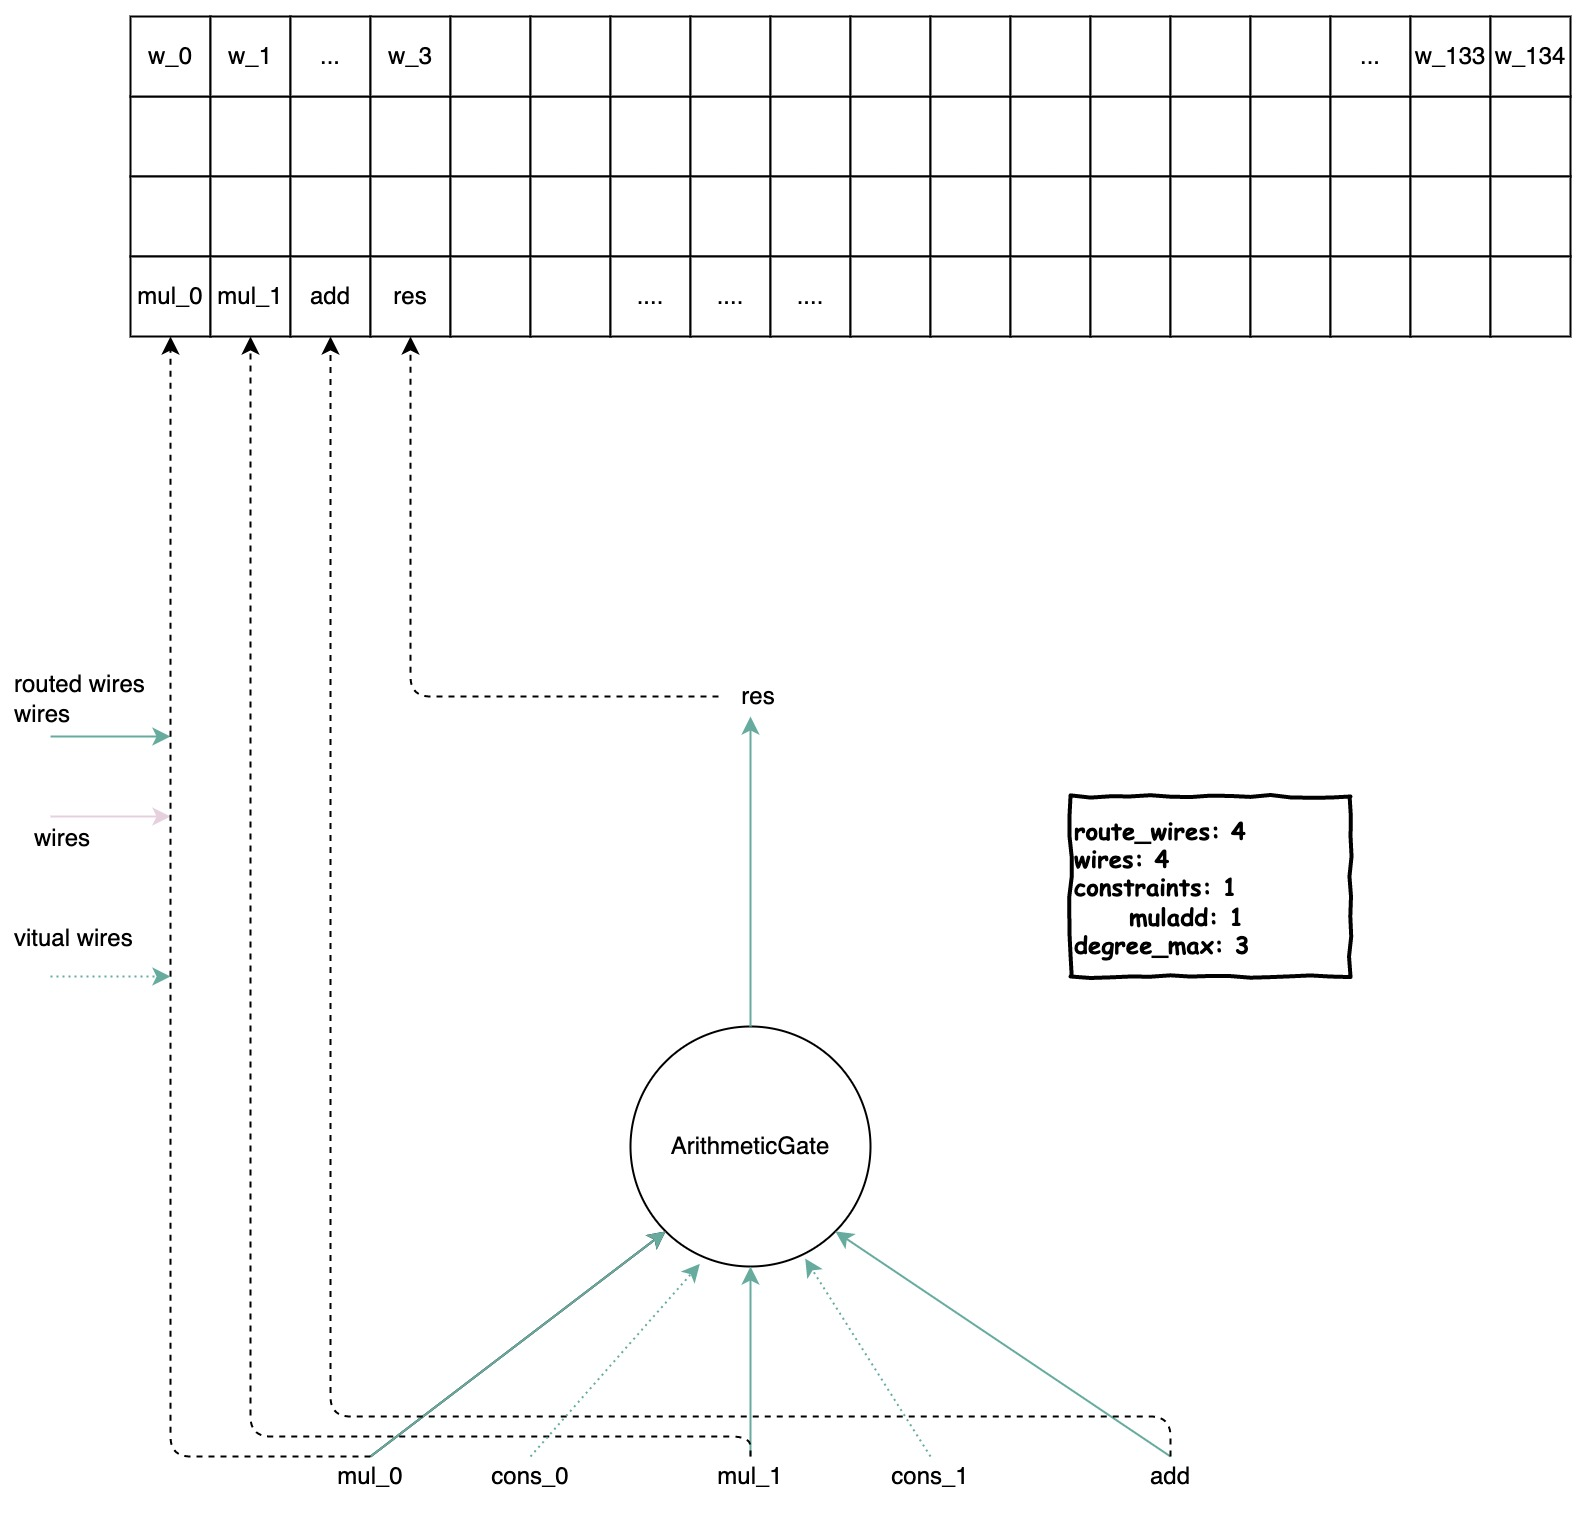
\includegraphics[width=0.5\textwidth]{gates/arithmetic_base.jpeg}
    \caption{ArithmeticGate}
    \label{fig:arithmetic-gate}
\end{figure}

There's only one constraint per operation, and degree is 3.

\subsubsubsection{arithmetic\_extension}

\hspace*{\fill}

\indent To understand the design principle of this Gate, we must first understand \href{https://en.wikipedia.org/wiki/Field_extension#Extension_field}{Field extension}. 

Taking Plonky2's Goldilocks field as an example, we give the extension field elements under quadratic, quartic, and quintic extensions respectively in \ref{fig:goldilocks field extension}.

\begin{figure}[!ht]
    \centering
    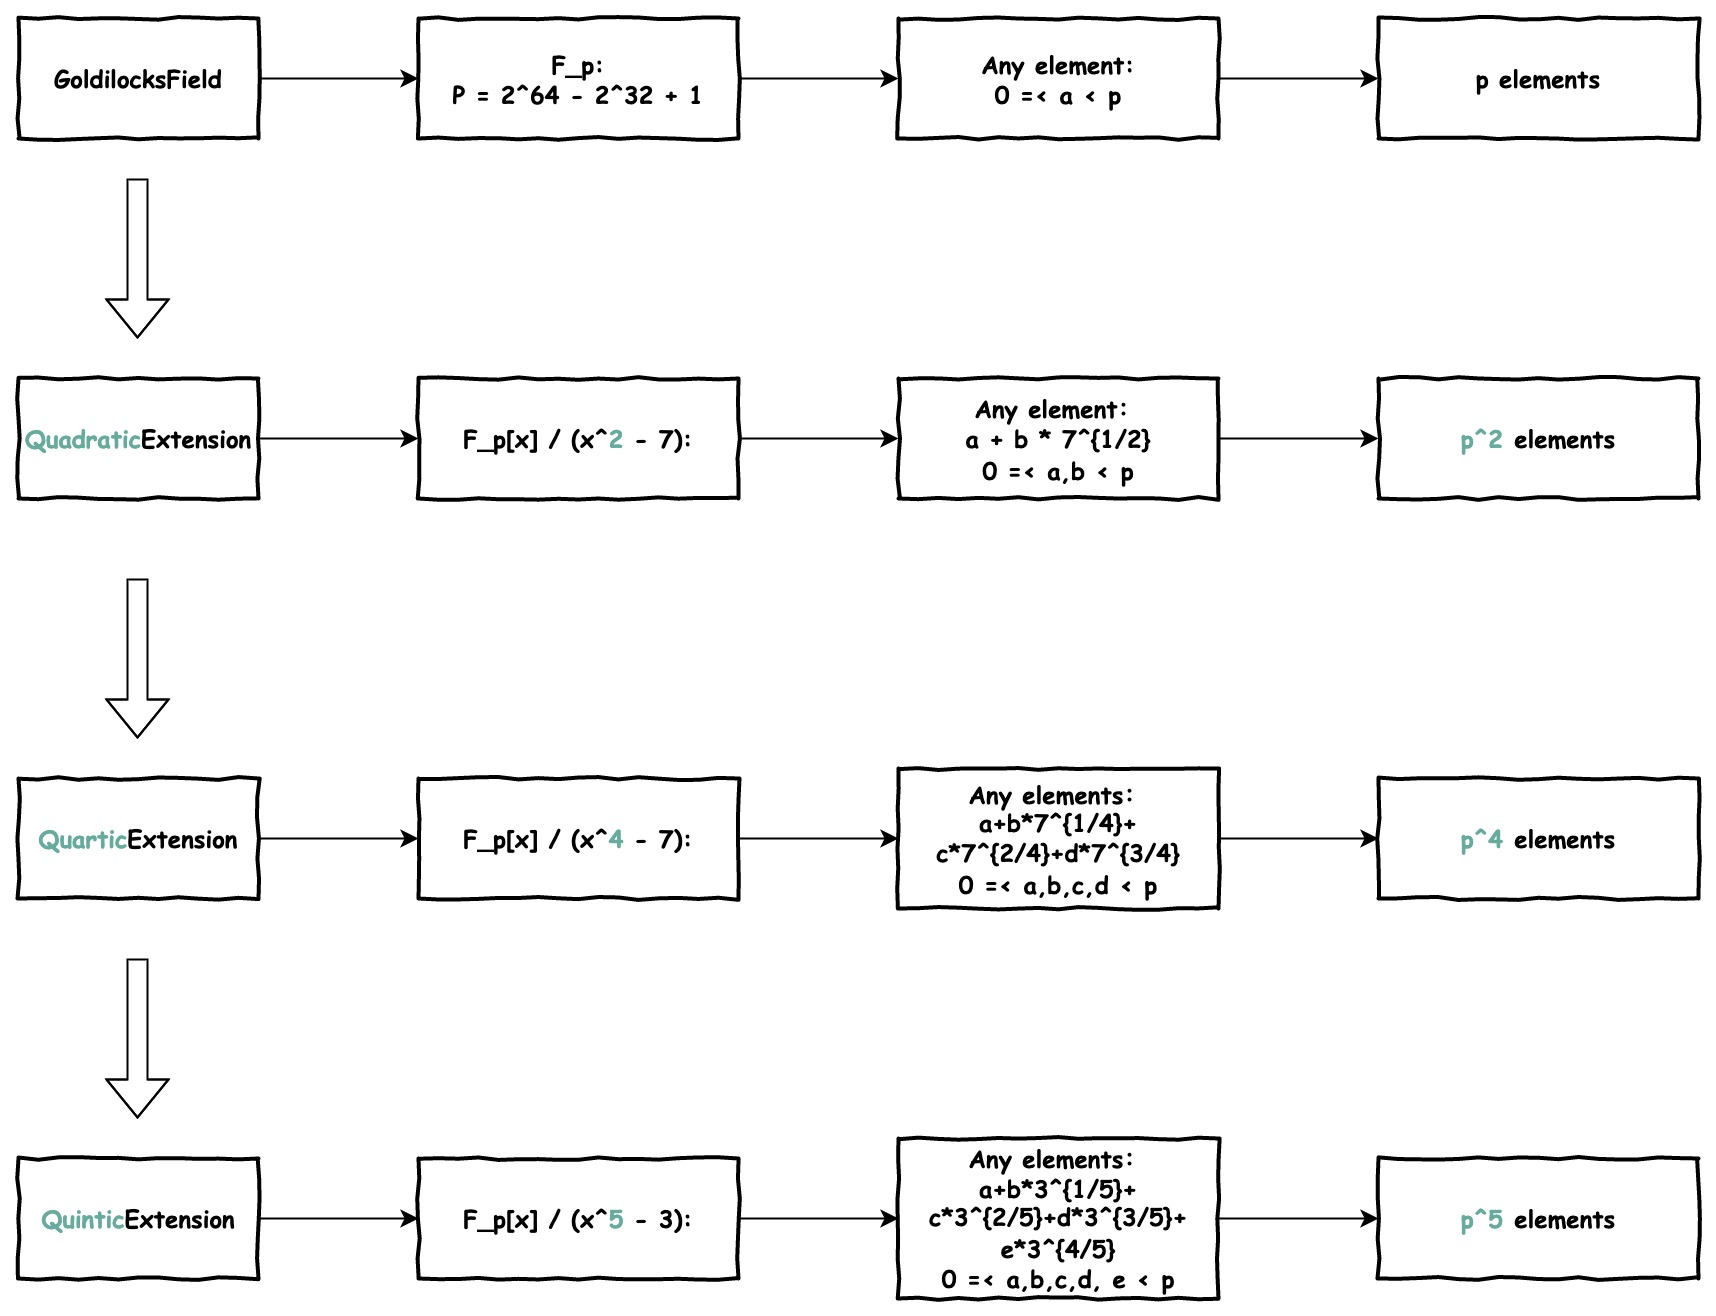
\includegraphics[width=0.6\textwidth]{gates/arthmetic_extension_ext.jpeg}
    \caption{Goldilocks Field Extension}
    \label{fig:goldilocks field extension}
\end{figure}

It is easy to see that for QuadraticExtension Field, the elements on its domain take the form $a+b\sqrt{7}, \ a,b \in F_p$.
It can be seen that on the quadratic extension domain, there are $p^2$ elements and the original domain is a subset of the quadratic extension domain.

ArithmeticExtensionGate is also a gate that can perform a weighted multiply-add, i.e.
\[ \text{res} = \text{cons\_0} \times \text{mul\_0} \times \text{mul\_1} + \text{cons\_1} \times \text{add} \]

The elements of the QuadraticExtension Field are represented in the form $[a, b]$, so the Gate design for arithmetic\_extension has the following form:

The structure of the gate is shown in \ref{fig:arthmetic-extension}. There's only one constraint per operation, and the degree is 3.
\begin{figure}[!ht]
    \centering
    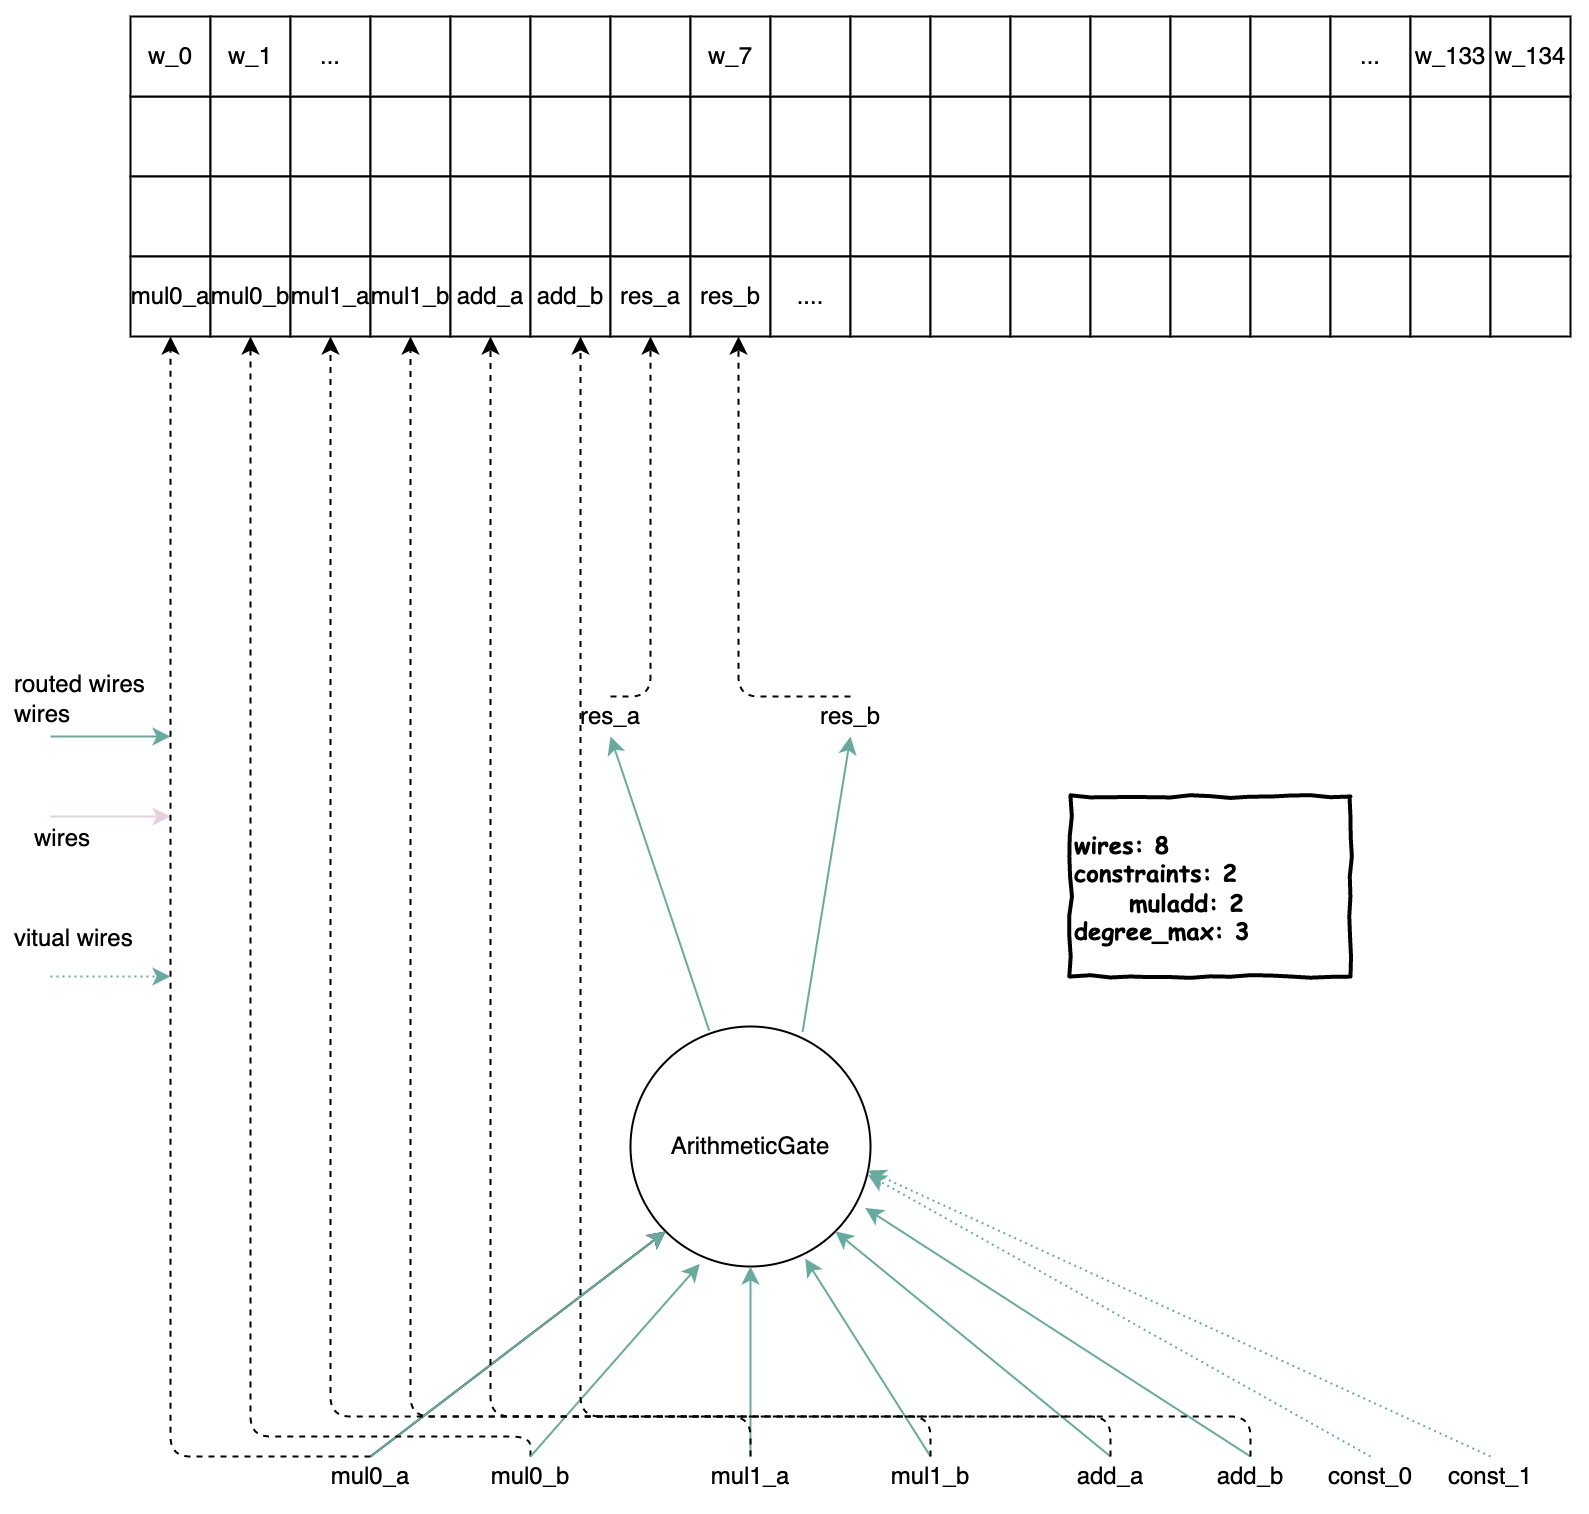
\includegraphics[width=0.6\textwidth]{gates/arthmetic_extension.jpeg}
    \caption{ArithmeticExtensionGate}
    \label{fig:arthmetic-extension}
\end{figure}
\paragraph{base\_sum}

BaseSumGate is used to constrain the input to be composed of limbs which are arranged in little-endian. There are two kinds of constraints:

For each limb, limb is in range $[0, \text{base})$:
\[ \sum_{i=0}^{\text{base}}(\text{limb}_i - i) = 0. \]

Input is composed of limbs:
\[ \text{input} = \sum_{i=0}^{n-1} \text{limb}_{n-1-i} \times \text{base}^i. \]

The structure of gate is shown in \figref{fig:base-sum}.
\begin{figure}[!ht]
    \centering
    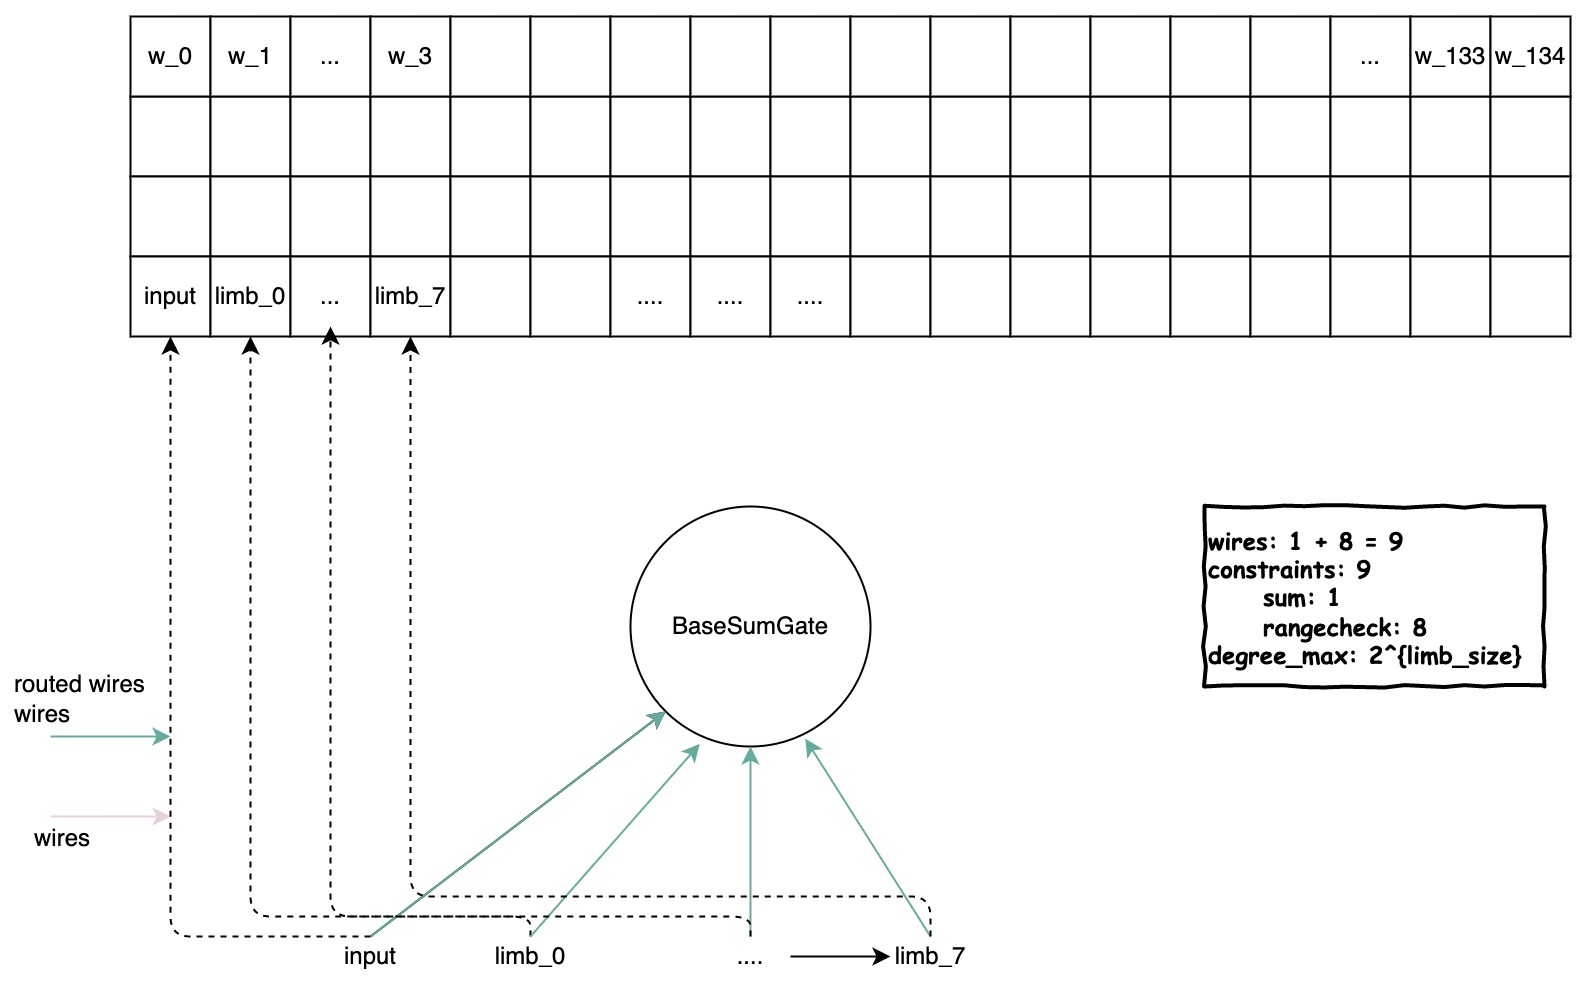
\includegraphics[width=0.8\textwidth]{gates/base_sum.jpeg}
    \caption{BaseSumGate}
    \label{fig:base-sum}
\end{figure}

There's 1 constraint for sum check and 8 constraints for limbs' range check. Degree of the gate is $2^{\text{limb\_size}}$ happens when limbs' range check.

\subsubsubsection{exponentiation}

\hspace*{\fill}

\indent ExponentiationGate is a gate for raising a value to a power. The trace table contains the base, bits of the exponent, output, and intermediate value of the bits.

Take $A^{21} = A^{10101_b}$ for example to describe intermediate value, the bits are [1, 0, 1, 0, 1].

\begin{enumerate}
    \item Current bit = 1, we start from 1, and times $A^{bit}$ we get $A$
    \item Current bit = 0,
    \begin{itemize}
        \item Square prev\_intermediate\_value $A^{1_b << 1} = A^{10_b}$
        \item Then times $A^{bit}$ we get $A^{10_b} \times A^0 = A^{10_b}$
    \end{itemize}
    \item Current bit = 1,
    \begin{itemize}
        \item Square prev\_intermediate\_value $A^{10_b << 1} = A^{100_b}$
        \item Then times $A^{bit}$ we get $A^{100_b} \times A = A^{101_b}$
    \end{itemize}
    \item Current bit = 0,
    \begin{itemize}
        \item Square prev\_intermediate\_value $A^{101_b << 1} = A^{1010_b}$
        \item Then times $A^{bit}$ we get $A^{1010_b} \times 1 = A^{1010_b}$
    \end{itemize}
    \item Current bit = 1,
    \begin{itemize}
        \item Square prev\_intermediate\_value $A^{1010_b << 1} = A^{10100_b}$
        \item Then times $A^{bit}$ we get $A^{10100_b} \times A = A^{10101_b}$
    \end{itemize}
\end{enumerate}

And we get the last intermediate value $A^{10101_b}$ which should be equal to the output.

Let's take another example of a specific number $2^{13} = 2^{1101_b}$, and have a look at the trace cell:
\begin{center}
    \begin{tabular}{ |c|c|c|c|c|c|c|c|c|c| }
        \hline
        base & b\_0 & b\_1 & b\_2 & b\_3 & output & inter\_0 & inter\_1 & inter\_2 & inter\_3 \\
        \hline
        2 & 1 & 0 & 1 & 1 & 8192 & 2 & 8 & 64 & 8192 \\
        \hline
    \end{tabular}
\end{center}

The structure of the gate is shown in \ref{fig:exponetiation-gate}.
\begin{figure}[!ht]
    \centering
    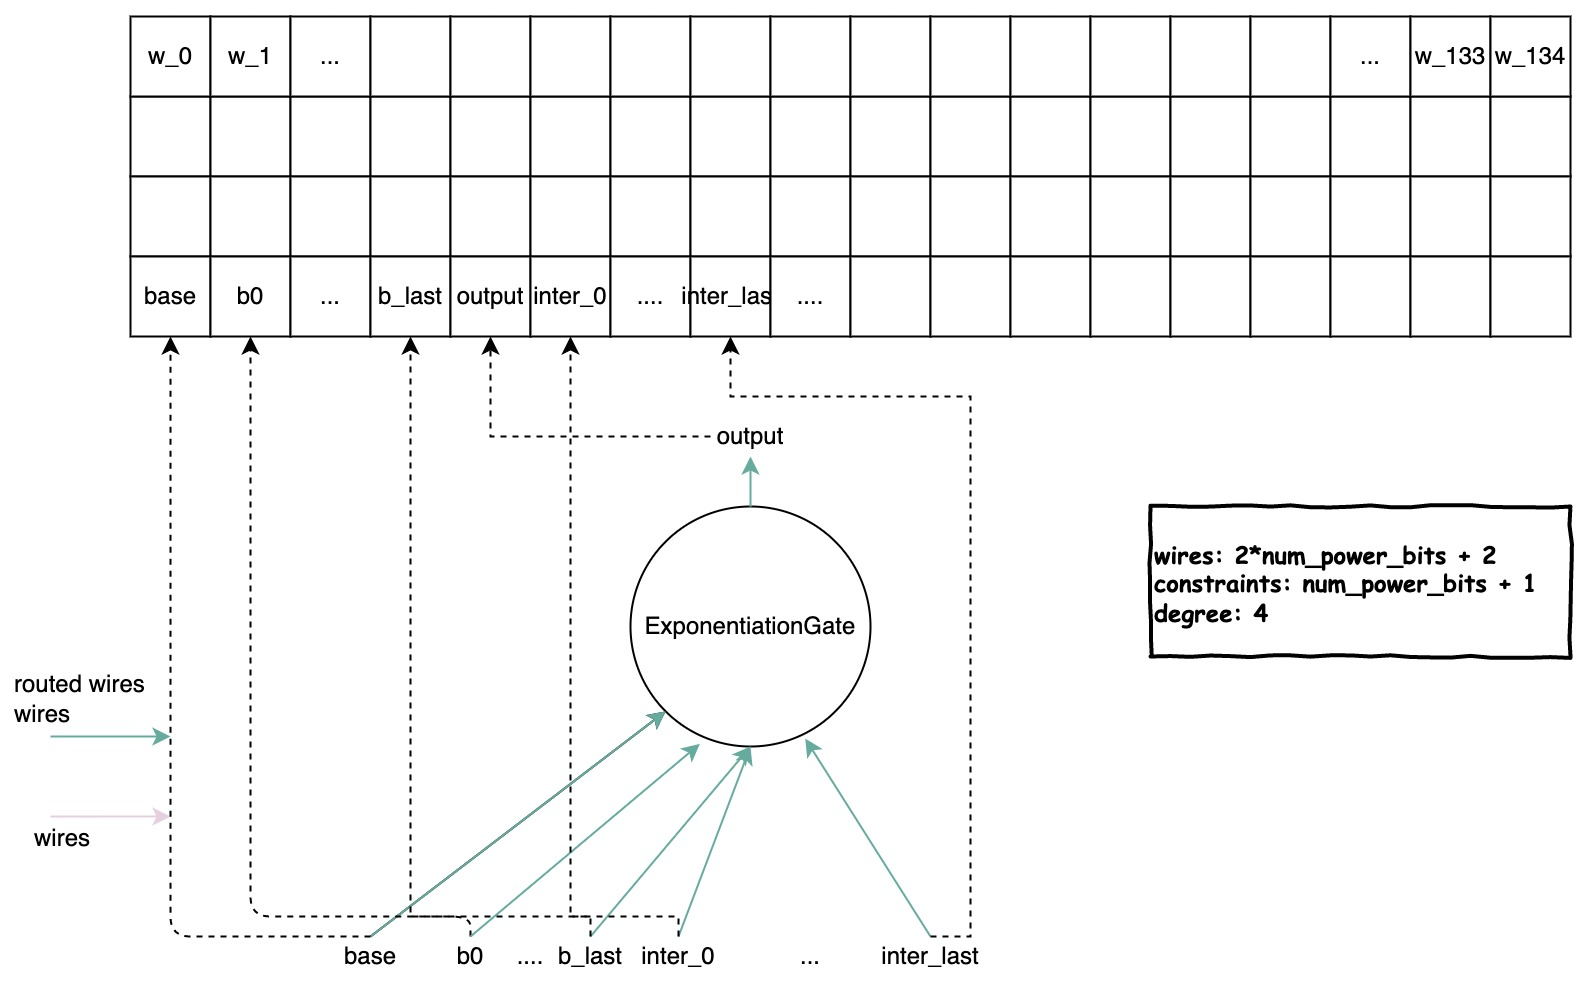
\includegraphics[width=0.6\textwidth]{gates/exponentiation.jpeg}
    \caption{ExponentiationGate}
    \label{fig:exponetiation-gate}
\end{figure}

Each step result is constrainted with intermediate values, and output is constrained with the final intermediated value, a total of $bits + 1$ constraints.
The degree of the gate is 4, which is determined by the intermediate calculation:
\begin{lstlisting}[language=rust]
let computed_intermediate_value =
            prev_intermediate_value * (cur_bit * base + not_cur_bit);
\end{lstlisting}

\paragraph{poseidon}

\href{https://www.poseidon-hash.info/}{Poseidon} is a hash function designed for the Zero-Knowledge proof system.
Its calculation process is rough as follows:

\begin{figure}[!ht]
    \centering
    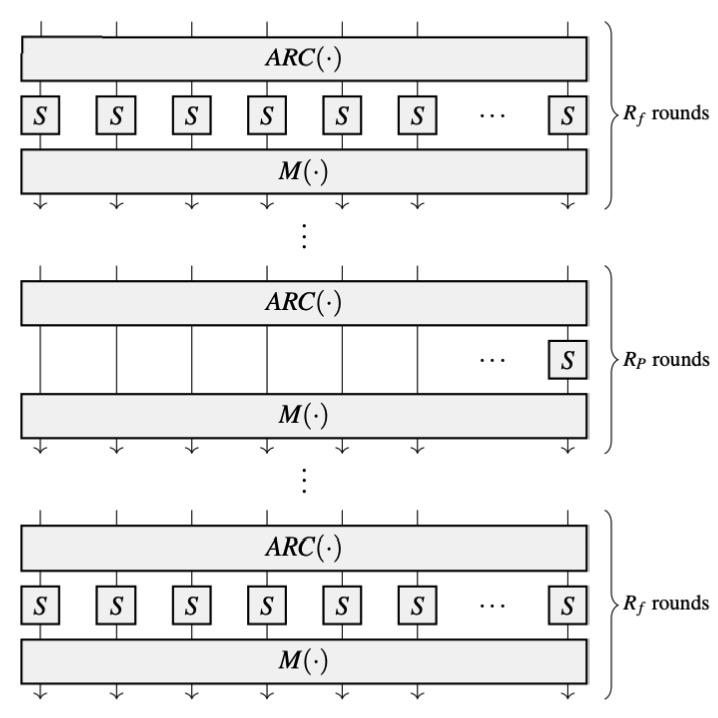
\includegraphics[width=0.6\textwidth]{gates/poseidon_process.jpeg}
    \caption{Construction of poseidon}
    \label{fig:poseidon-process}
\end{figure}

Each round function of Poseidon permutation consists of the following three components.
\begin{enumerate}
    \item ARC(.): AddRoundConstants
    \item S: SubWords
    \item M(.): MixLayer
\end{enumerate}

The Trace of the gate is like this:
\begin{figure}[!ht]
    \centering
    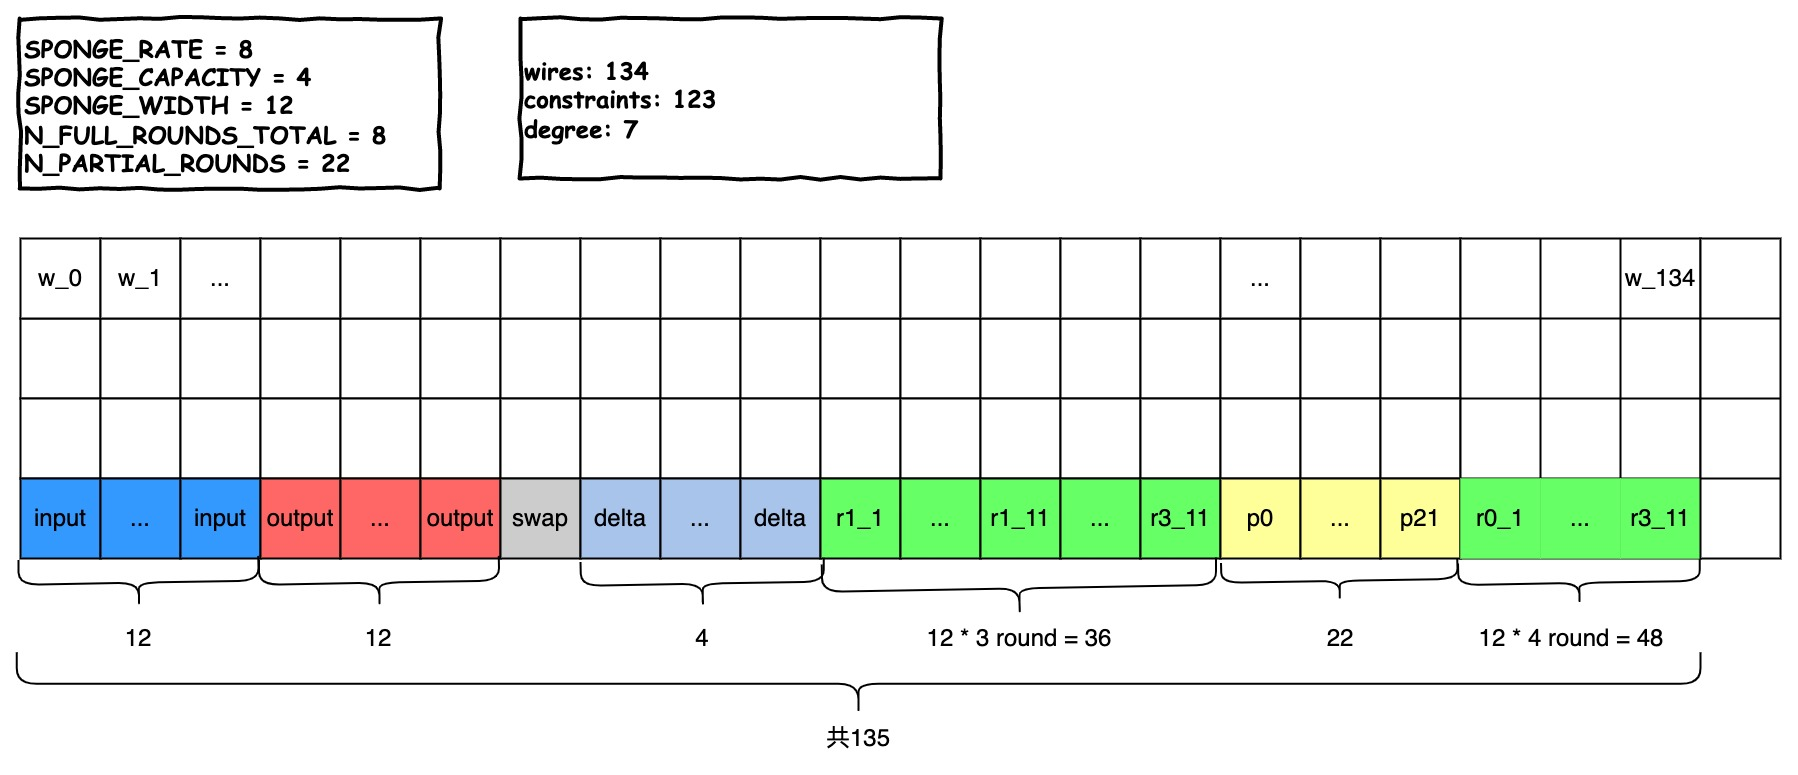
\includegraphics[width=0.6\textwidth]{gates/poseidon.jpeg}
    \caption{PoseidonGate}
    \label{fig:poseidon-gate}
\end{figure}

\begin{itemize}
    \item input: components of the input, 12 elements.
    \item output: components of the output, 12 elements.
    \item swap: 0 or 1, Indicates whether the first four elements of the input are swapped with the last four elements.
    \item delta: used when swap is 1, $\text{delta}_i = \text{swap} \times (\text{input}_{\text{rhs}} - \text{input}_{\text{lhs}})$.
    \item green region: full rounds, ri\_1~ri\_11 is the state of each round.
    \item yellow region: partial rounds, each element is state[0] of each round.
\end{itemize}

Calculation process and related constraints:
\begin{itemize}
    \item Assert that swap is binary. (1 constraint)
    \begin{lstlisting}[language=rust]
constraints.push(swap * (swap - F::Extension::ONE))
    \end{lstlisting}
    \item Assert $\text{delta}_i = \text{swap} \times (\text{rhs} - \text{lhs})$. (4 constraints)
    \begin{lstlisting}[language=rust]
for i in 0..4 {
    ....
    constraints.push(swap * (input_rhs - input_lhs) - delta_i);
}
    \end{lstlisting}
    \item Initialize state: when swap=0, state=input; when swap=1, state is swapped input:
    \begin{figure}[!ht]
        \centering
        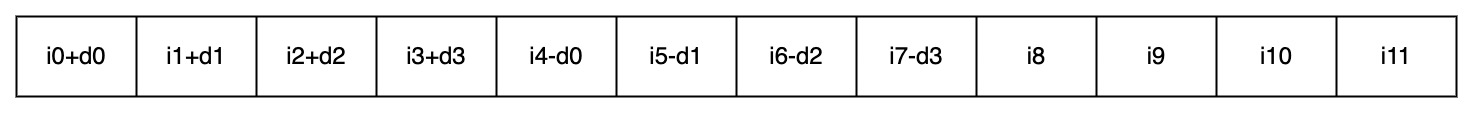
\includegraphics[width=0.6\textwidth]{gates/poseidon_state_init.jpeg}
        \caption{Poseidon State Init}
        \label{fig:poseidon-state-init}
    \end{figure}
    \begin{lstlisting}[language=rust]
for i in 0..4 {
    ...
    state[i] = vars.local_wires[input_lhs] + delta_i;
    state[i + 4] = vars.local_wires[input_rhs] - delta_i;
}
for i in 8..SPONGE_WIDTH {
    state[i] = vars.local_wires[Self::wire_input(i)];
}
    \end{lstlisting}
    \item Begin first full rounds calculation, for each round r (which is 0--3):
    \begin{itemize}
        \item Perform ARC: Add each element of state to the pre-generated value at a particular position in the array.
        \begin{lstlisting}[language=rust]
for i in 0..WIDTH {
    state[i] += F::from_canonical_u64(ALL_ROUND_CONSTANTS[i + WIDTH * round_ctr]);
}
        \end{lstlisting}
        \item Except for r=0, constrain each element of the state calculated in the previous round (the green part of the first slice of the figure). 
        (12 constraints per round, a total of 36 constraints)
        \item Perform SubWords: Turn state element by element x into $x \mapsto x^7$
        \item Perform MixLayer: Each element of the state is updated according to itself and a pre-generated array.
        \begin{lstlisting}[language=rust]
// r is the index of state elements here.
let mut res = F::ZERO;
    for i in 0..WIDTH {
    res += v[(i + r) % WIDTH] * F::from_canonical_u64(Self::MDS_MATRIX_CIRC[i]);
}
res += v[r] * F::from_canonical_u64(Self::MDS_MATRIX_DIAG[r]);
        \end{lstlisting}
    \end{itemize}
    \item Perform partial rounds:
    \begin{itemize}
        \item Perform ARC
        \begin{lstlisting}[language=rust]
for i in 0..12 {
    if i < WIDTH {
        state[i] += F::from_canonical_u64(Self::FAST_PARTIAL_FIRST_ROUND_CONSTANT[i]);
    }
}
        \end{lstlisting}
        \item Processing of state with $11 \times 11$ MDS (maximum distance separable) matrix.
        \begin{lstlisting}[language=rust]
result[0] = state[0];
for r in 1..12 {
    if r < WIDTH {
        for c in 1..12 {
            if c < WIDTH {
                let t = F::from_canonical_u64(
                    Self::FAST_PARTIAL_ROUND_INITIAL_MATRIX[r - 1][c - 1],
                );
                result[c] += state[r] * t;
            }
        }
    }
}
result
        \end{lstlisting}
        \item Perform 22 round sbox, for the first 21 rounds (r = 0--21):
        \begin{itemize}
            \item Take sbox\_in(yellow elements in the figure), and constrains state[0]=sbox\_in -- 21 rounds totally 21 constraints.
            \item \verb|state[0] = state[0]^7|
            \item \verb|state[0] += FAST_PARTIAL_ROUND_CONSTANTS[r]|
            \item Perform mds to state.
        \end{itemize}
        \item For the 22th round:
        \begin{itemize}
            \item \verb|state[0] = sbox_in| (i constraint)
            \item \verb|state[0] = state[0]^7|
            \item Perform mds to state.
        \end{itemize}
    \end{itemize}
    \item Perform second round "Full rounds", same with the first round. (the green part of the second slice of the figure). (12 constraints, 4 rounds totally of 48 constraints)
    \item Asserts computed result equals output. (12 constraints)
    \begin{lstlisting}[language=rust]
for i in 0..SPONGE_WIDTH {
    constraints.push(state[i] - vars.local_wires[Self::wire_output(i)]);
}
    \end{lstlisting}
\end{itemize}

The constraints of this gate in total is 123, the degree is 7 (when performing s-box, making $\text{state}[i] \mapsto \text{state}[i]^7$).

\paragraph{poseidon\_mds}

\hspace*{\fill}

\indent This gate is used for constraining outputs of Poseidon mds.

\begin{figure}[!ht]
    \centering
    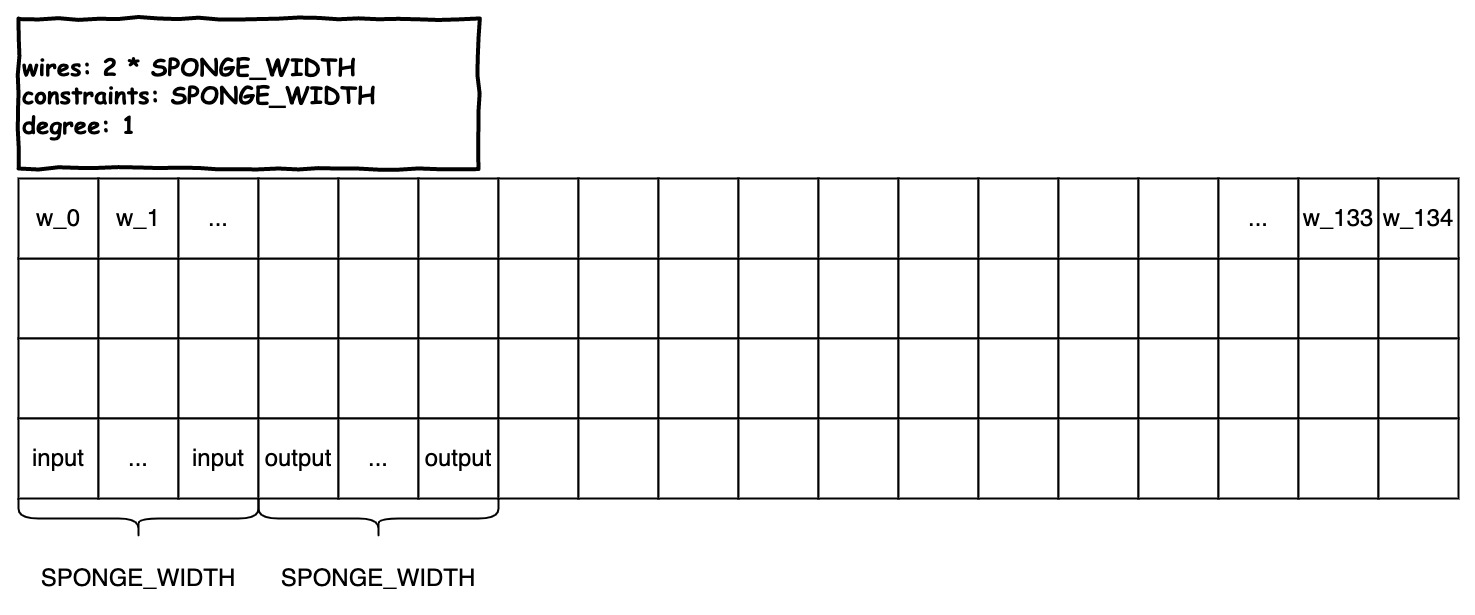
\includegraphics[width=0.6\textwidth]{gates/poseidon_mds.jpeg}
    \caption{PoseidonMdsGate}
    \label{fig:poseidon-mds}
\end{figure}

computed\_output is calculated from input, and constrained with output element by element, a total of 12 constraints (degree 1).
\begin{lstlisting}[language=rust]
let inputs: [_; SPONGE_WIDTH] = (0..SPONGE_WIDTH)
    .map(|i| vars.get_local_ext_algebra(Self::wires_input(i)))
    .collect::<Vec<_>>()
    .try_into()
    .unwrap();
let computed_outputs = Self::mds_layer_algebra(&inputs);
(0..SPONGE_WIDTH)
    .map(|i| vars.get_local_ext_algebra(Self::wires_output(i)))
    .zip(computed_outputs)
    .flat_map(|(out, computed_out)| (out - computed_out).to_basefield_array())
    .collect()
\end{lstlisting}

\paragraph{random\_access}

RandomAccessGate is used to verify that an element matches a value in the list.

\begin{figure}[!ht]
    \centering
    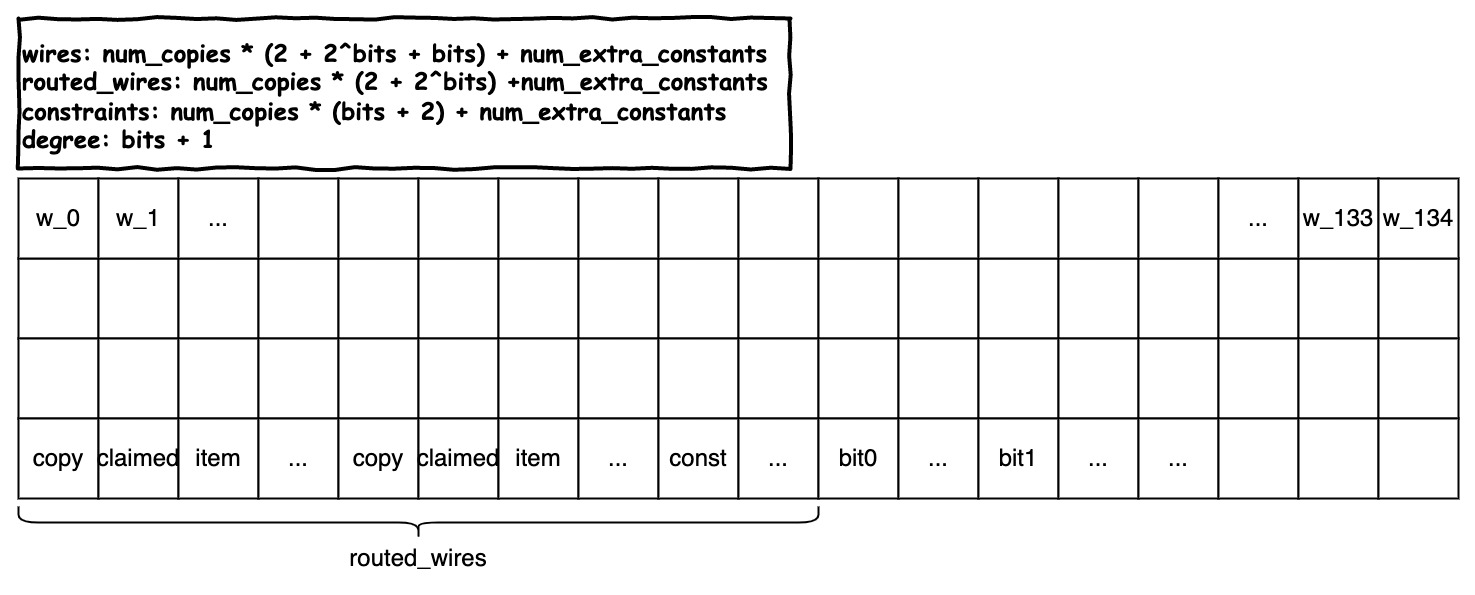
\includegraphics[width=0.6\textwidth]{gates/random_access.jpeg}
    \caption{RandomAccessGate}
    \label{fig:random-access}
\end{figure}

\begin{itemize}
    \item item: list items.
    \item copy: index of the target element in the list
    \item claimed: target element
    \item bit\_i: bits for the i-th copy
\end{itemize}

For each copy:
\begin{itemize}
    \item Constrain bits are 0 or 1. -- bits constraints for each copy, A total of num\_copied*bits constraints.
    \begin{lstlisting}[language=rust]
for &b in &bits {
    constraints.push(builder.mul_sub_extension(b, b, b));
}
    \end{lstlisting}
    \item Constraint copy consists of bits. -- 1 constraint for each copy, A total of num\_copied constraints.
    \begin{lstlisting}[language=rust]
let reconstructed_index = bits
    .iter()
    .rev()
    .fold(zero, |acc, &b| builder.mul_add_extension(acc, two, b));
constraints.push(builder.sub_extension(reconstructed_index, access_index));
    \end{lstlisting}
    \item For each bit, reconstruct items with a 2-elements-tuple, select the first element when the bit is 0, and select the second when the bit is 1.
    After the bits round, only one element remains, that is, the index element corresponding to bits, constraint it with claimed.
    \begin{figure}[!ht]
        \centering
        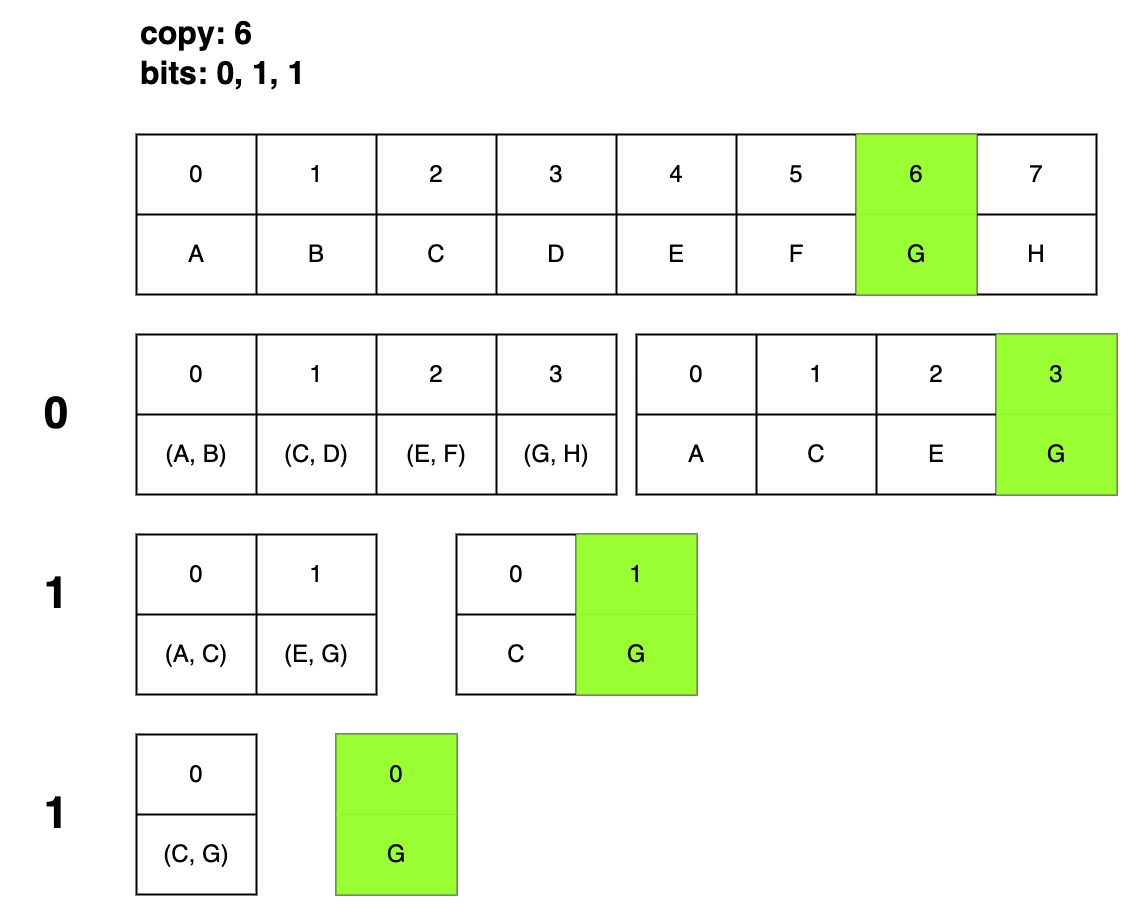
\includegraphics[width=0.6\textwidth]{gates/random_access_example.jpeg}
        \caption{Random Access Example}
        \label{fig:random-access-example}
    \end{figure}
    \begin{lstlisting}[language=rust]
for b in bits {
    list_items = list_items
        .iter()
        .tuples()
        .map(|(&x, &y)| builder.select_ext_generalized(b, y, x))
        .collect()
}
// Check that the one remaining element after the folding is the claimed element.
debug_assert_eq!(list_items.len(), 1);
constraints.push(builder.sub_extension(list_items[0], claimed_element));
    \end{lstlisting}
\end{itemize}

Finally, the constant is constrained -- A total of num\_extra\_constraints constraints.

In summary, there're $\text{num\_copies} \times (\text{bits} + 2) + \text{num\_extra\_constants}$ constraints. The degree is $\text{bits} + 1$ which happens when repeatedly folding the list. 

\paragraph{reducing}

ReducingGate is used for computes $\text{output} = \text{old\_acc} + \sum C_i*\alpha^i$ in base field.

Trace structure for this gate is like:

\begin{figure}[!ht]
    \centering
    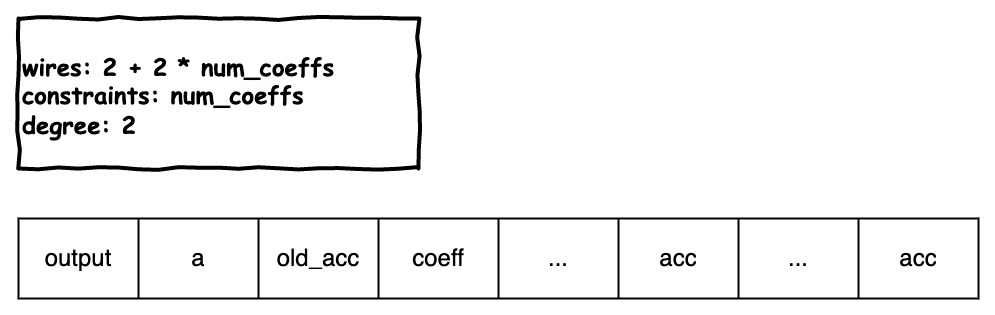
\includegraphics[width=0.5\textwidth]{gates/reducing.jpeg}
    \caption{ReducingGate}
    \label{fig:reducing}
\end{figure}

The constraint flow is relatively intuitive, initializing acc to old\_acc, then cumulative computation of polynomials by coeff in turn, 
and constraining the intermediate results of each step with acc.

\begin{lstlisting}[language=rust]
for i in 0..self.num_coeffs {
    let coeff = builder.convert_to_ext_algebra(coeffs[i]);
    let mut tmp = builder.mul_add_ext_algebra(acc, alpha, coeff);
    tmp = builder.sub_ext_algebra(tmp, accs[i]);
    constraints.push(tmp);
    acc = accs[i];
}
\end{lstlisting}

The number of constraints is equal to the number of coefficients. Polynomial degree is 2 which happens when calculating $\text{coeff}_i * \alpha$, sum up does not increase degree.

ReducingExtensionGate is like ReducingGate, just computations happen in extension field, constrain logic is all the same.

\paragraph{high\_degree\_interpolation}

InterpolationGate is used for interpolation a polynomial, whose points are a (base field) coset of the multiplicative subgroup 
with the given size, and whose values are extension field elements. As for HighDegreeInterpolationGate,  allows constraints of variable degree, 
up to \verb|1 << subgroup_bits|. The higher degree is a tradeoff for less gates (than LowDegreeInterpolationGate).


HighDegreeInterpolationGate trace is shown in \figref{fig:high-degree-interpolation}.

\begin{figure}[!ht]
    \centering
    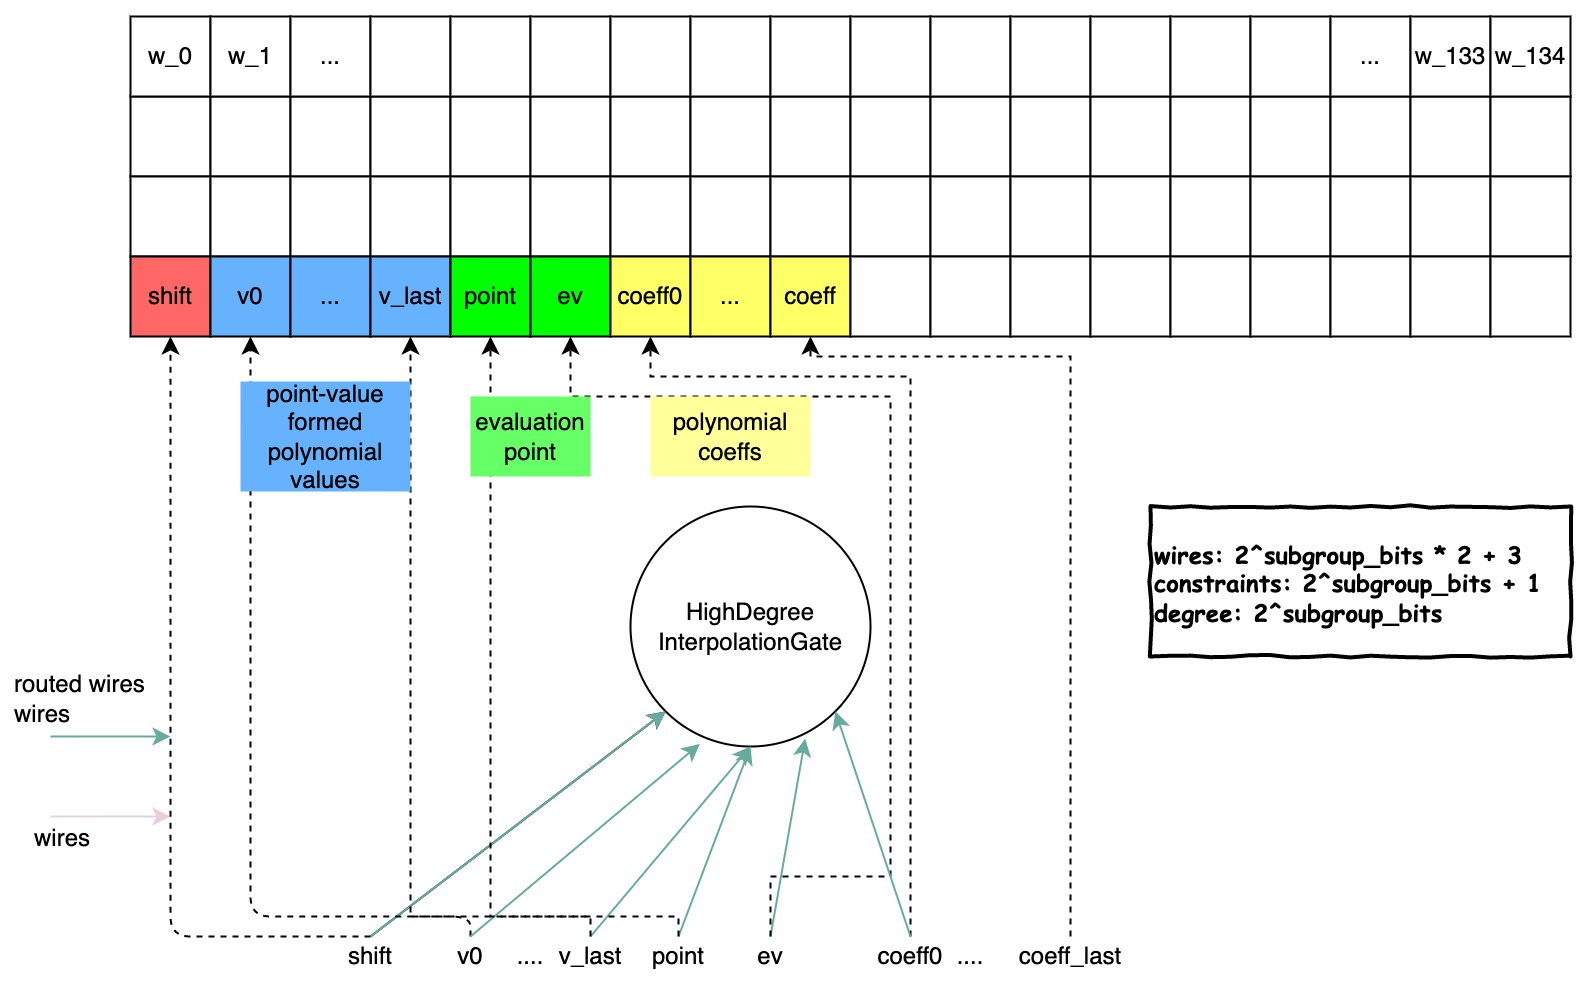
\includegraphics[width=0.6\textwidth]{gates/high_degree_interpolation.jpeg}
    \caption{HighDegreeInterpolationGate}
    \label{fig:high-degree-interpolation}
\end{figure}


Constraints:
\begin{itemize}
    \item Bring each point(from the point-value pairs) into the coefficient polynomial to compute the computed\_value, 
    and compare the constraint with the value(from the point-value pairs). -- A total of $2^{\text{subgroup\_bits}}$ constraints.
    \begin{lstlisting}
for (i, point) in coset.into_iter().enumerate() {
    let value = vars.get_local_ext_algebra(self.wires_value(i));
    let computed_value = interpolant.eval_base(point);
    constraints.extend((value - computed_value).to_basefield_array());
}
    \end{lstlisting}
    coset: $[sg, sg^2,...,sg^{2^{\text{subgroup\_bits}}}], \ s=\text{shift}$
    \item Evaluate the coefficient-form polynomial at evaluation point, and constrain with ev. -- 1 constraint.
\end{itemize}

The degree of this gate equals the number of points (num\_points): max point power is $\text{num\_points} - 1$, and multiplication by coefficient adds 1 degree.

Number of constraints equals $\text{num\_points} + 1$: num\_points for consistency between the coefficients and the point-value pairs, 1 constraints for the evaluation value. 

\paragraph{low\_degree\_interpolation}

InterpolationGate is used for the interpolation of a polynomial, whose points are a (base field) coset of the multiplicative subgroup 
with the given size, and whose values are extension field elements. As for LowDegreeInterpolationGate,  all constraints are degree <= 2, 
low degree is a tradeoff for more gates(than HighDegreeInterpolationGate).

LowDegreeInterpolationGate trace is shown in \figref{fig:low-degree-interpolation}.

\begin{figure}[!ht]
    \centering
    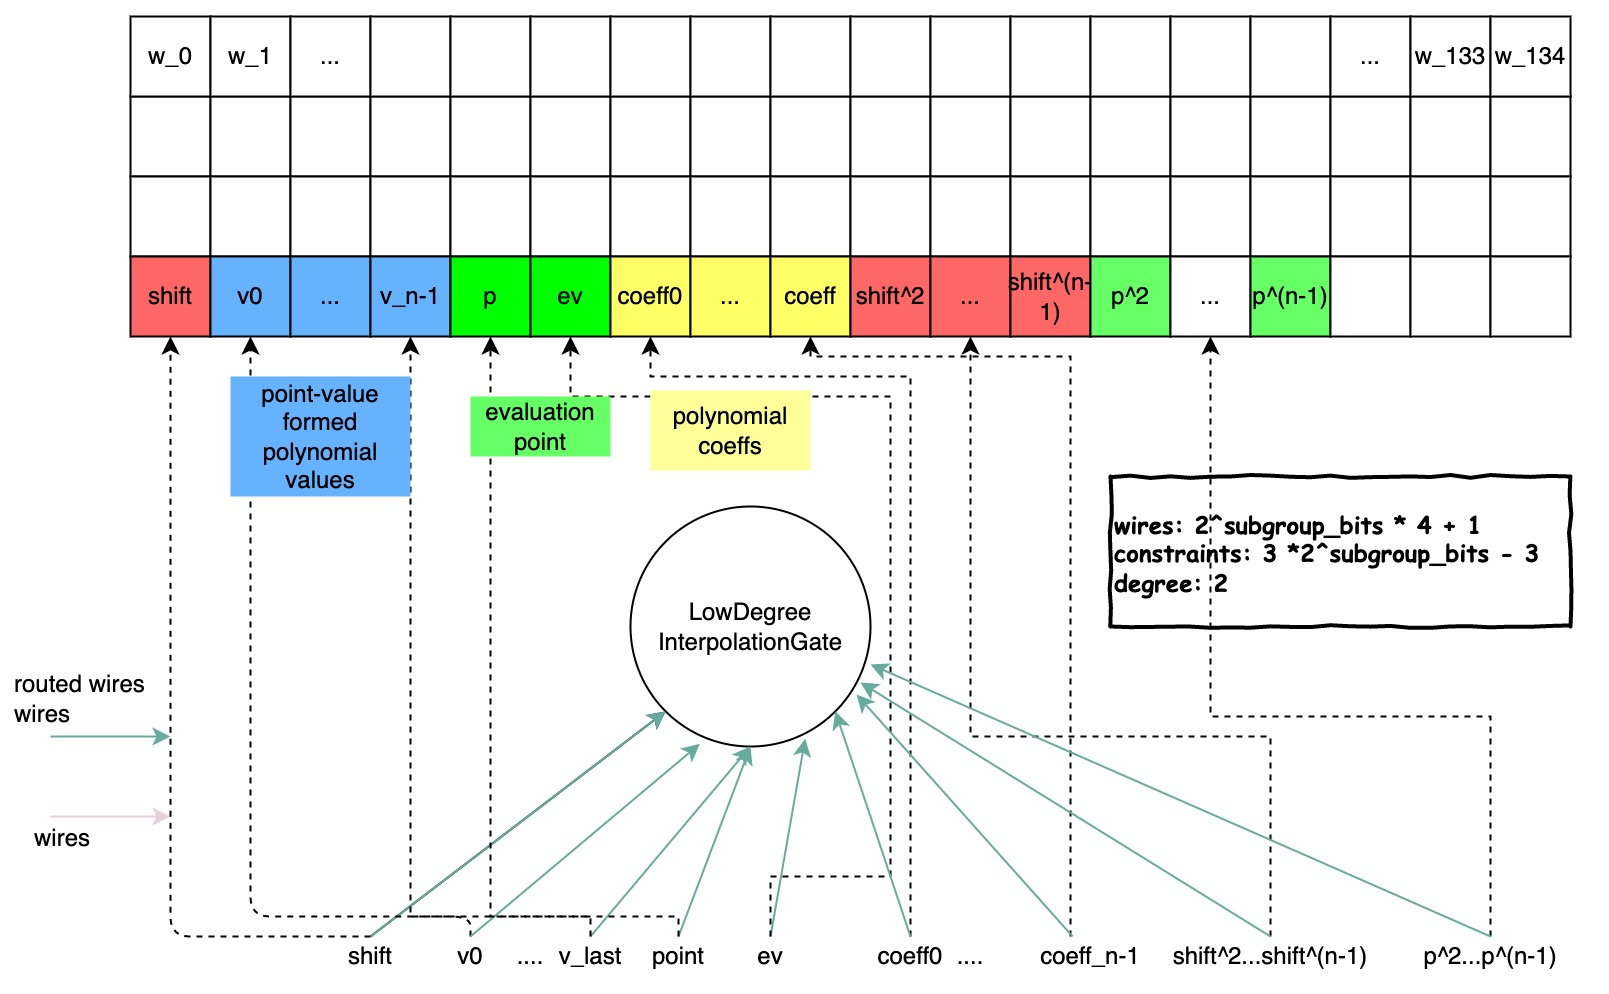
\includegraphics[width=0.6\textwidth]{gates/low_degree_interpolation.jpeg}
    \caption{LowDegreeInterpolationGate}
    \label{fig:low-degree-interpolation}
\end{figure}

Constraints:
\begin{itemize}
    \item Constrain powers of shift, from $\text{shift}^2$ to $\text{shift}^{n-1}$, a total of $2^{\text{subgroup\_bits}}-2$ constraints.
    \begin{lstlisting}[language=rust]
for i in 1..self.num_points() - 1 {
    constraints.push(powers_shift[i - 1] * shift - powers_shift[i]);
}
    \end{lstlisting}
    \item Bring each point (from the point-value pairs) into the coefficient polynomial to compute the computed\_value 
    and compare the constraint with the value (from the point-value pairs). -- A total of $2^{\text{subgroup\_bits}}$ constraints.
    \item Constrain powers of evaluation point. -- A total of $2^{\text{subgroup\_bits}}-2$ constraints.
    \item Evaluate the coefficient-form polynomial at the evaluation point and constrain it. -- 1 constraint.
\end{itemize}

As can be seen from the above constraint description, the number of constraints is $3*2^{\text{subgroup\_bits}}-3$, degree of LowDegreeInterpolationGate is 2.

\subsubsubsection{U32 gates}
\subsubsubsection{add\_many\_u32}

\hspace*{\fill}

\indent U32AddManyGate is a gate to perform addition on num\_addends different 32-bit values, plus a small carry. 
There can be up to 16 operations per gate.

The gate structure is like \figref{fig:add-many-u32}.

\begin{figure}[!ht]
    \centering
    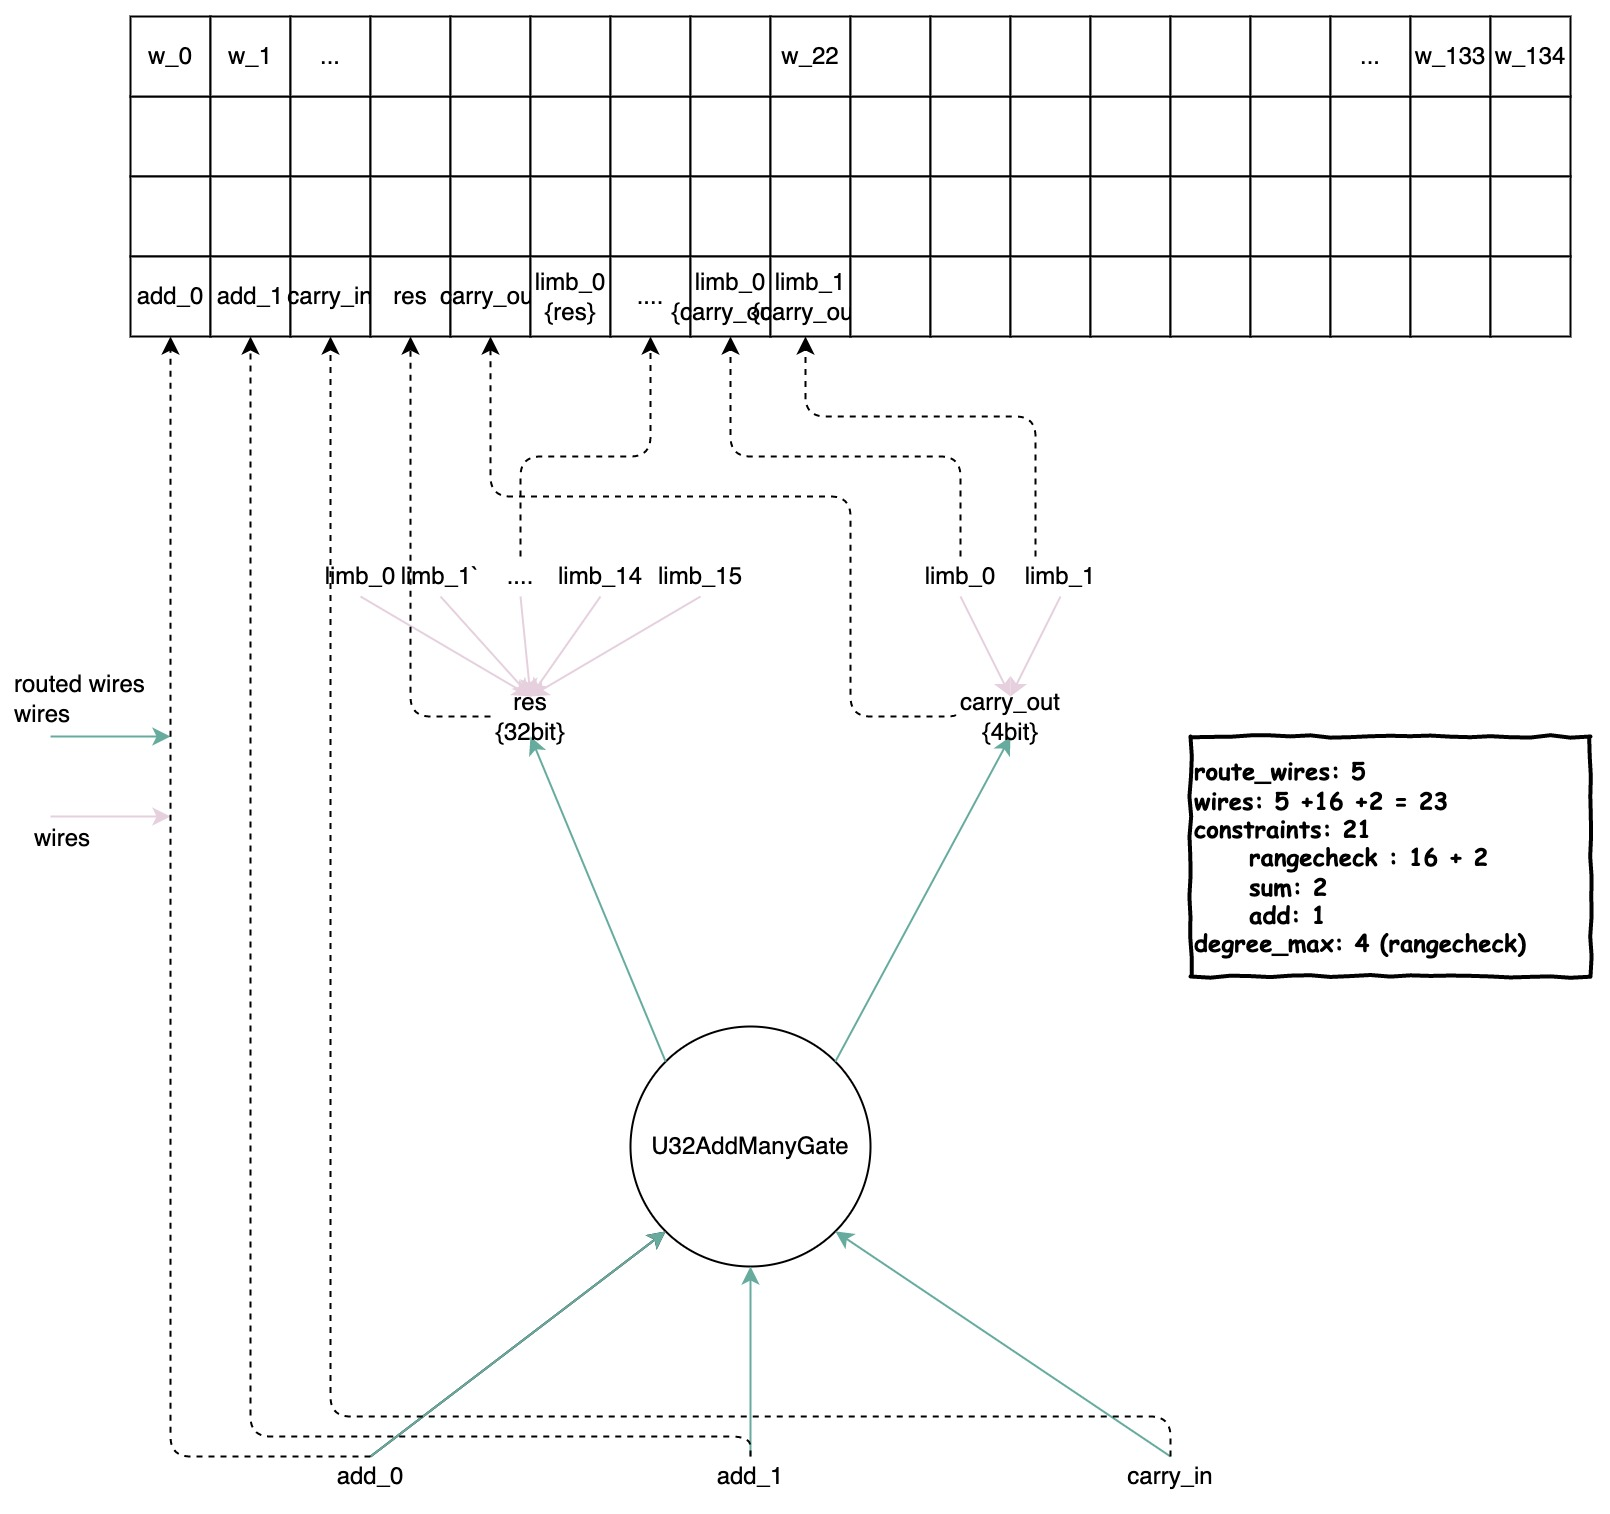
\includegraphics[width=0.6\textwidth]{gates/add_many_u32.jpeg}
    \caption{U32AddManyGate}
    \label{fig:add-many-u32}
\end{figure}

Constraints for each operation:
\begin{itemize}
    \item Constrain the result of addends summation equals results of res and carry\_out calculation. -- 1 constraint with degree 1
    \begin{lstlisting}[language=rust]
let base = F::Extension::from_canonical_u64(1 << 32u64);
let combined_output = output_carry * base + output_result;
constraints.push(combined_output - computed_output);
    \end{lstlisting}
    \item Limbs range check. -- 18(limbs) constraints with degree 4.(limbs are all 2-bits)
    \begin{lstlisting}[language=rust]
let product = (0..max_limb)
    .map(|x| this_limb - F::Extension::from_canonical_usize(x))
    .product();
constraints.push(product);
    \end{lstlisting}
    \item Constrain limbs for res and carry\_out. -- 2 constraints with degree 1.
\end{itemize}

In summary, there are 21 constraints for each operation. The degree of the gate is 4 which is needed by the 4-bits limbs range check.

\paragraph{arithmetic\_u32}

U32ArithmeticGate gate is used for compute $\text{res} = \text{mul\_0} \times \text{mul\_1} + \text{add}$. Res is store in res\_lo and res\_hi each of which can be represented by 15 limbs.

Gate structure is like \figref{fig:arithmetic-u32}.

\begin{figure}[!ht]
    \centering
    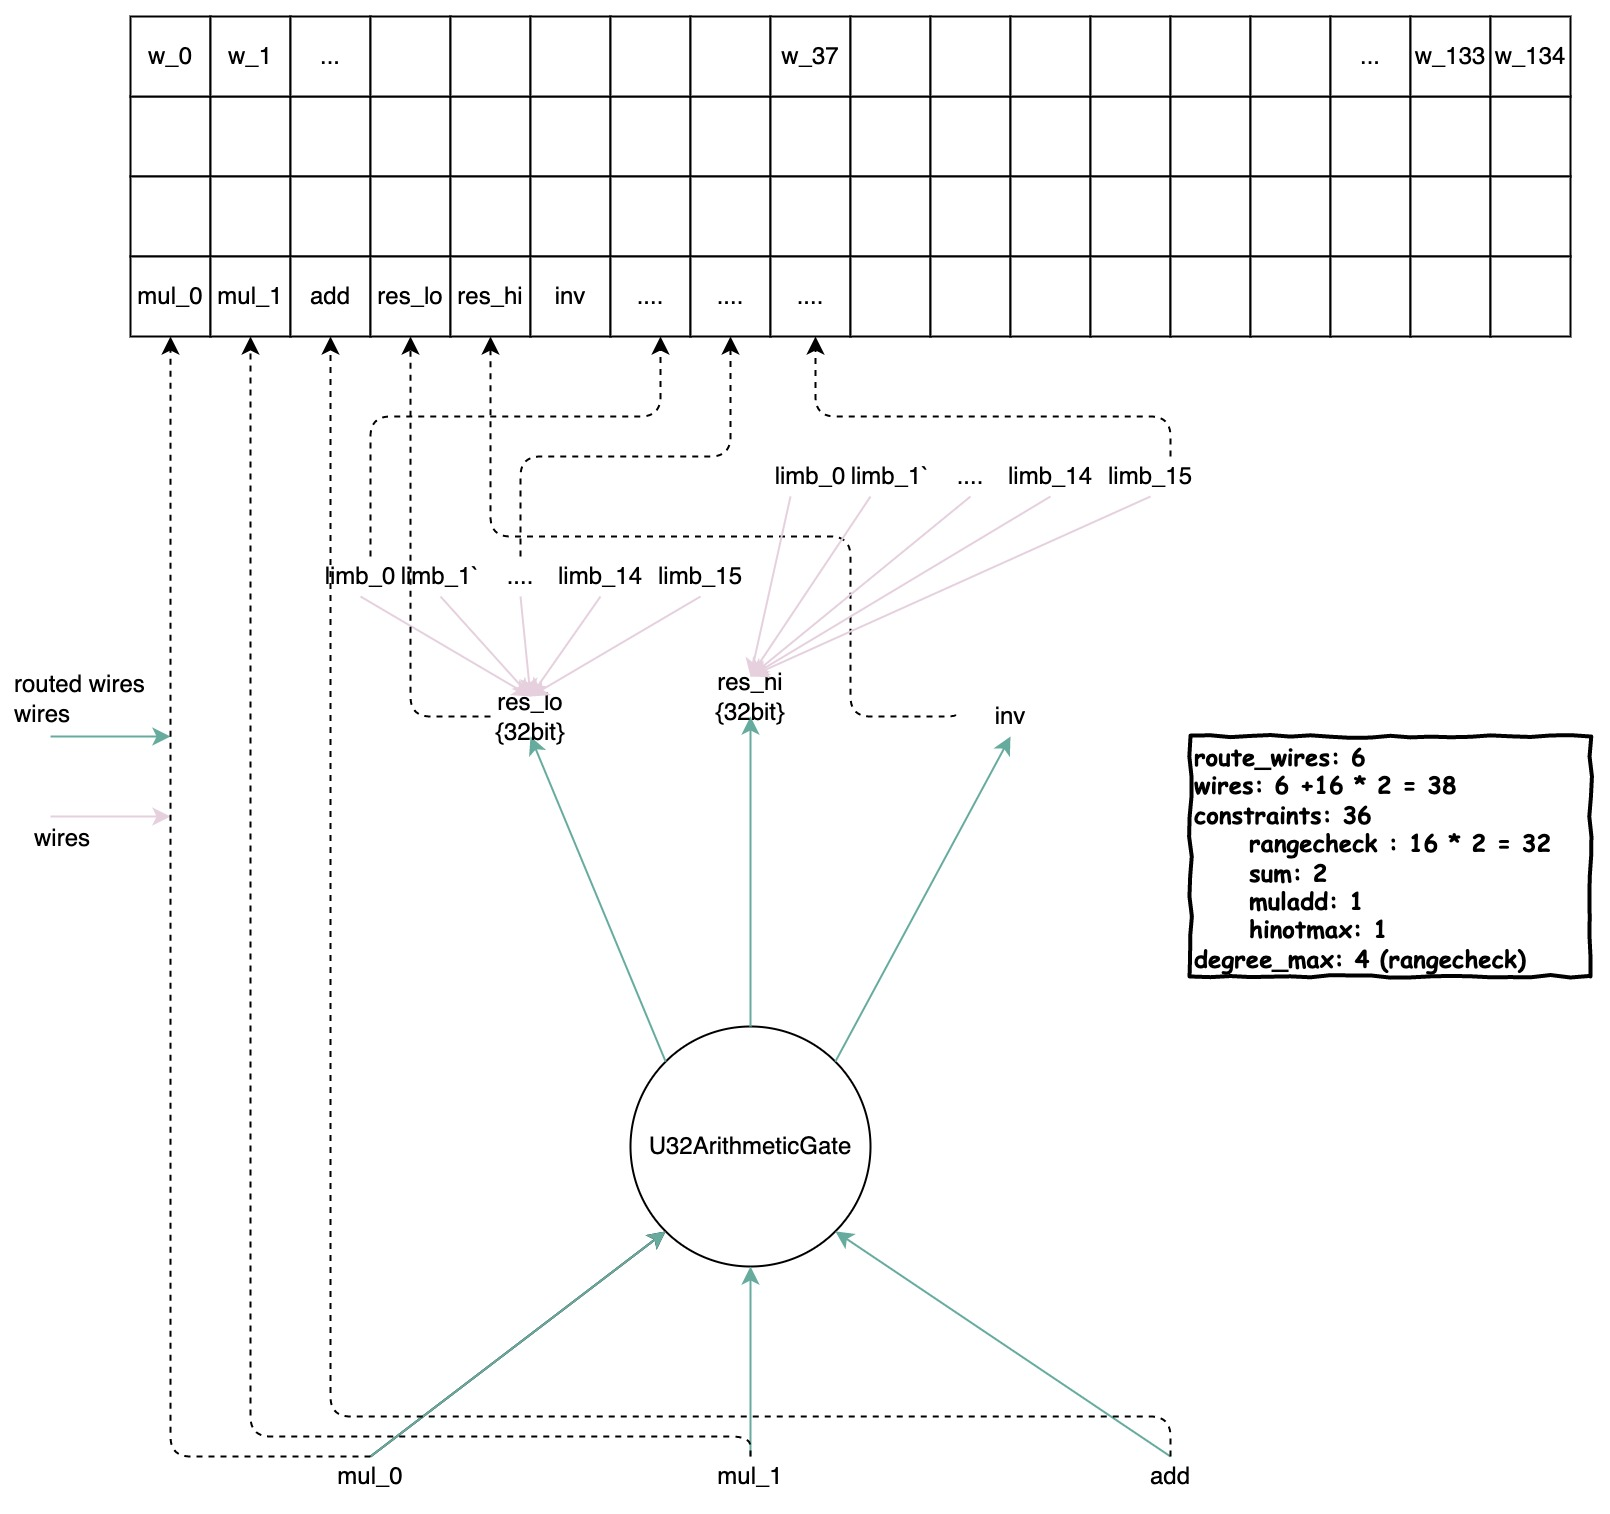
\includegraphics[width=0.8\textwidth]{gates/arithmetic_u32.jpeg}
    \caption{U32ArithmeticGate}
    \label{fig:arithmetic-u32}
\end{figure}

Constraints for each operation:
\begin{itemize}
    \item Constrain res is not overflow (less equal than \verb|max_u32 * max_u32 + max_u32|). -- 1 constraint with degree 2.
    \item Constrain combined((by res\_lo and res\_hi)) output equals computed (by \verb|mul_0 * mul_1 + add|) output. -- 1 constraint with degree 2.
    \item Limbs range check. -- 32 (limbs) constraints with degree 4. (limbs are all 2-bits)
    \item Constrain limbs for res\_lo and res\_hi. -- 2 constraints with degree 1.
\end{itemize}

In summary, there are 36 constraints for each operation. Degree of the gate is 4 which is needed by 4-bits limbs range check.

\subsubsubsection{comparison}

\hspace*{\fill}

\indent ComparisonGate is a gate for checking that one value is less than or equal to another. 
Compared numbers are divided into chunks, and chunk size and the number are configurable.

For a ComparisonGate with 8 4-bits chunks is like \figref{fig:comparison}.

\begin{figure}[!ht]
    \centering
    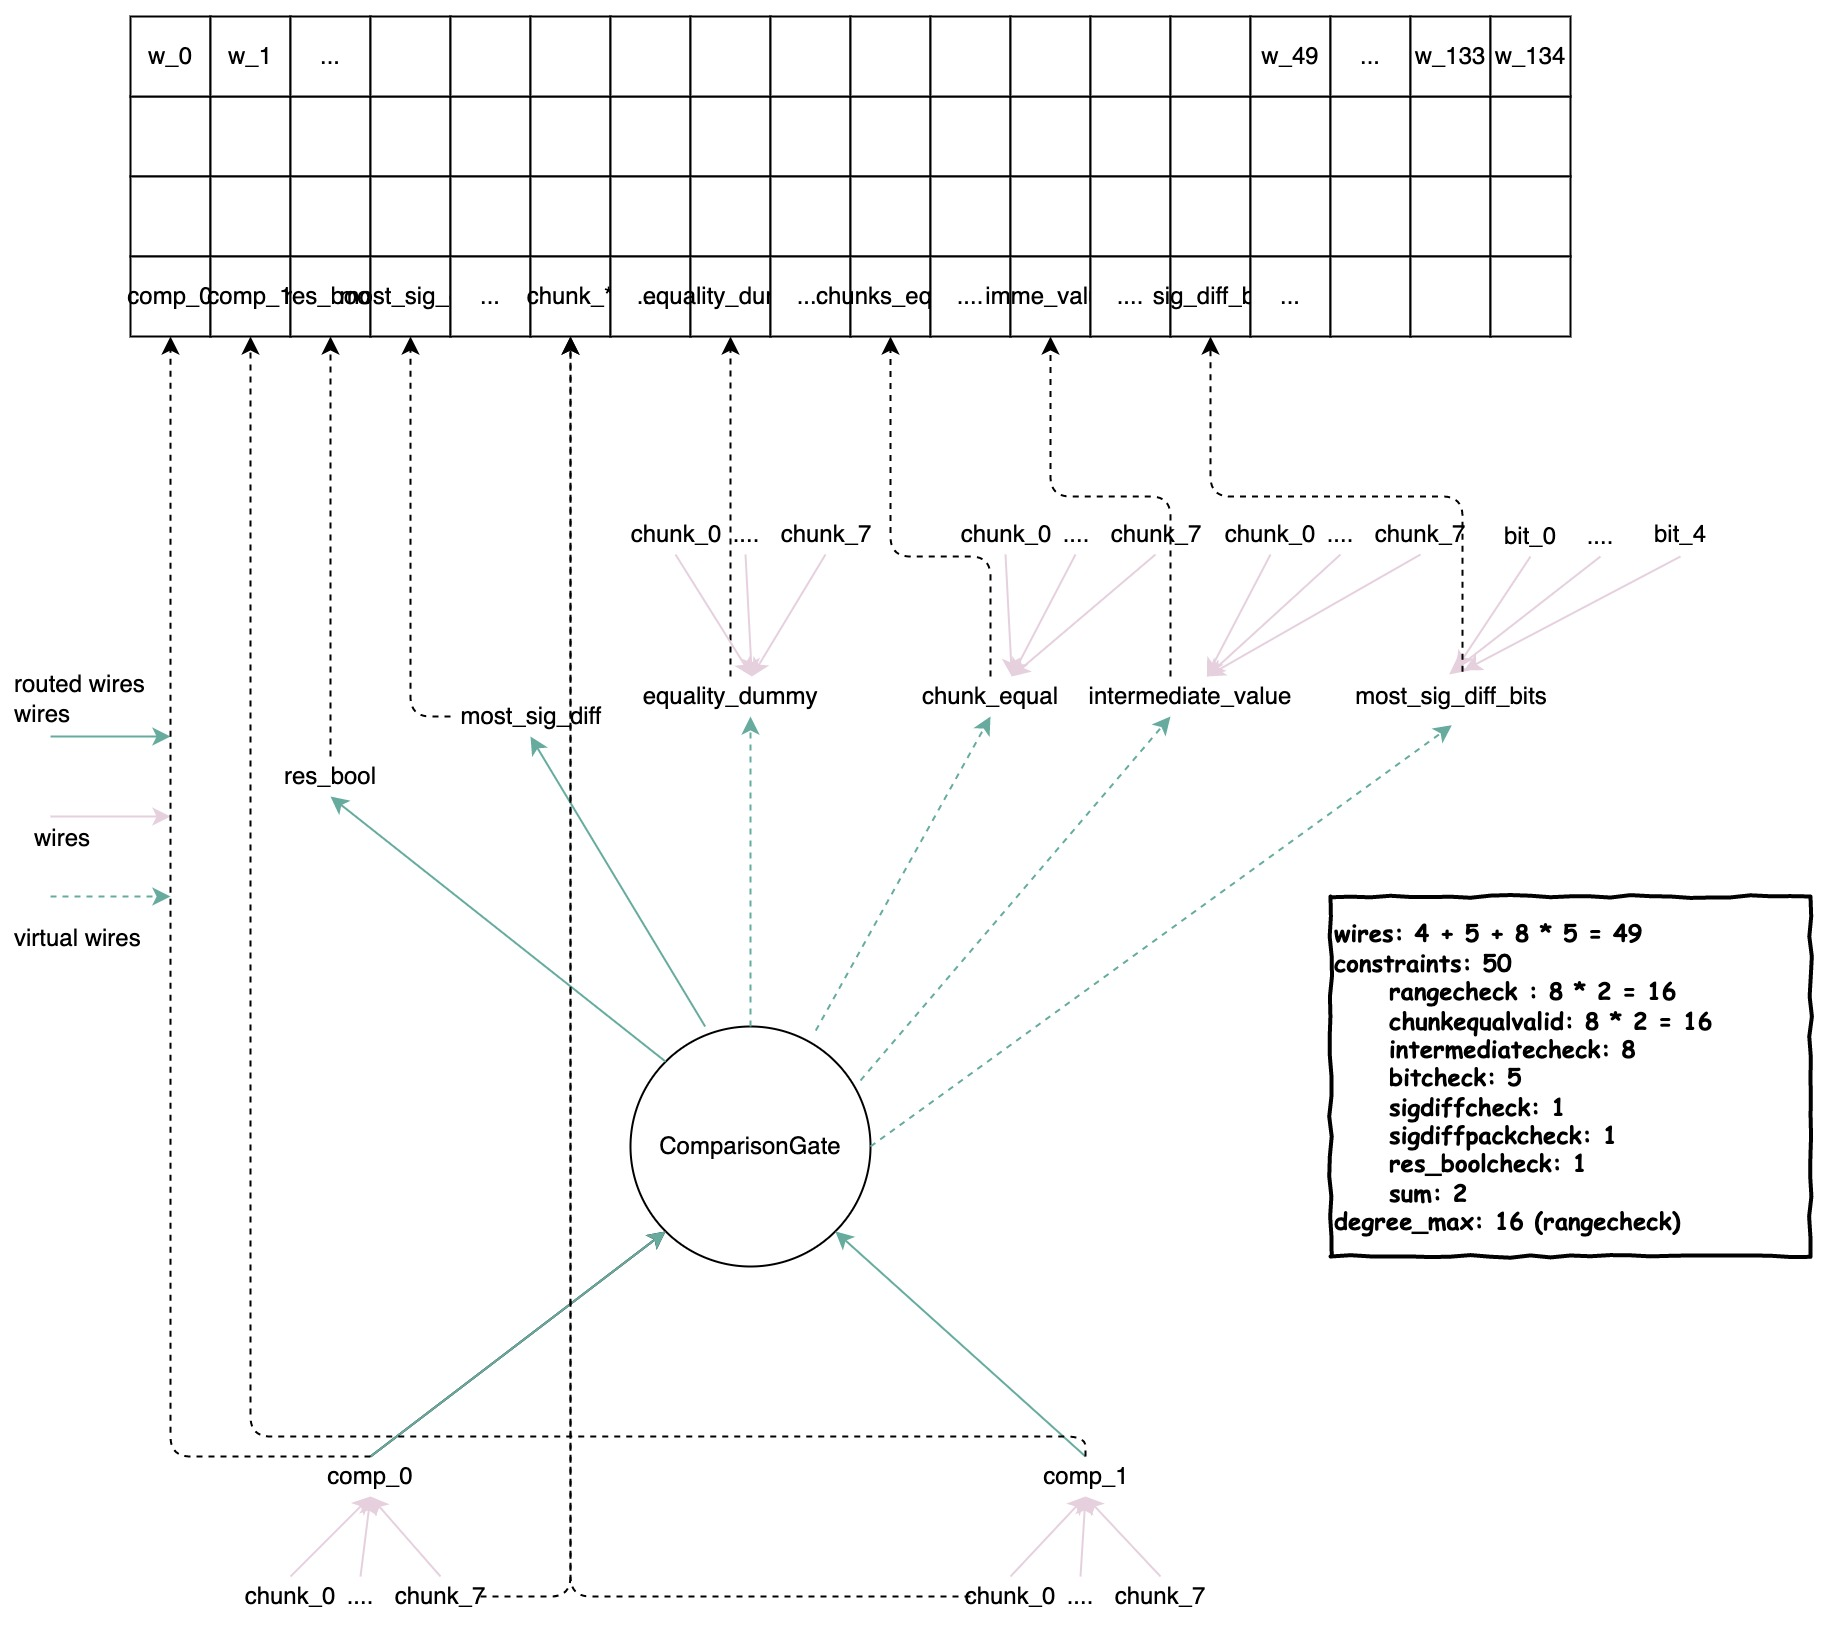
\includegraphics[width=0.6\textwidth]{gates/comparison.jpeg}
    \caption{ComparisonGate}
    \label{fig:comparison}
\end{figure}

The main idea of constraints:
\begin{itemize}
    \item Consistency of the sliced chunks and the original values.
    \item Range check for each chunk.
    \item If the chunks are equal, the difference is 0 and there is no inverse.
    \item Chunk by chunk so for most significant diff equals related intermediate\_value.
    \item If first <= second, the top \verb|n+1|-th bit of $(2^n + \text{most\_significant\_diff})$ will be 1.
\end{itemize}

\paragraph{range\_check\_u32}

U32RangeCheckGate is a gate that can decompose a number into base B little-endian limbs.

The gate structure is like \figref{fig:range-check-u32}.

\begin{figure}[!ht]
    \centering
    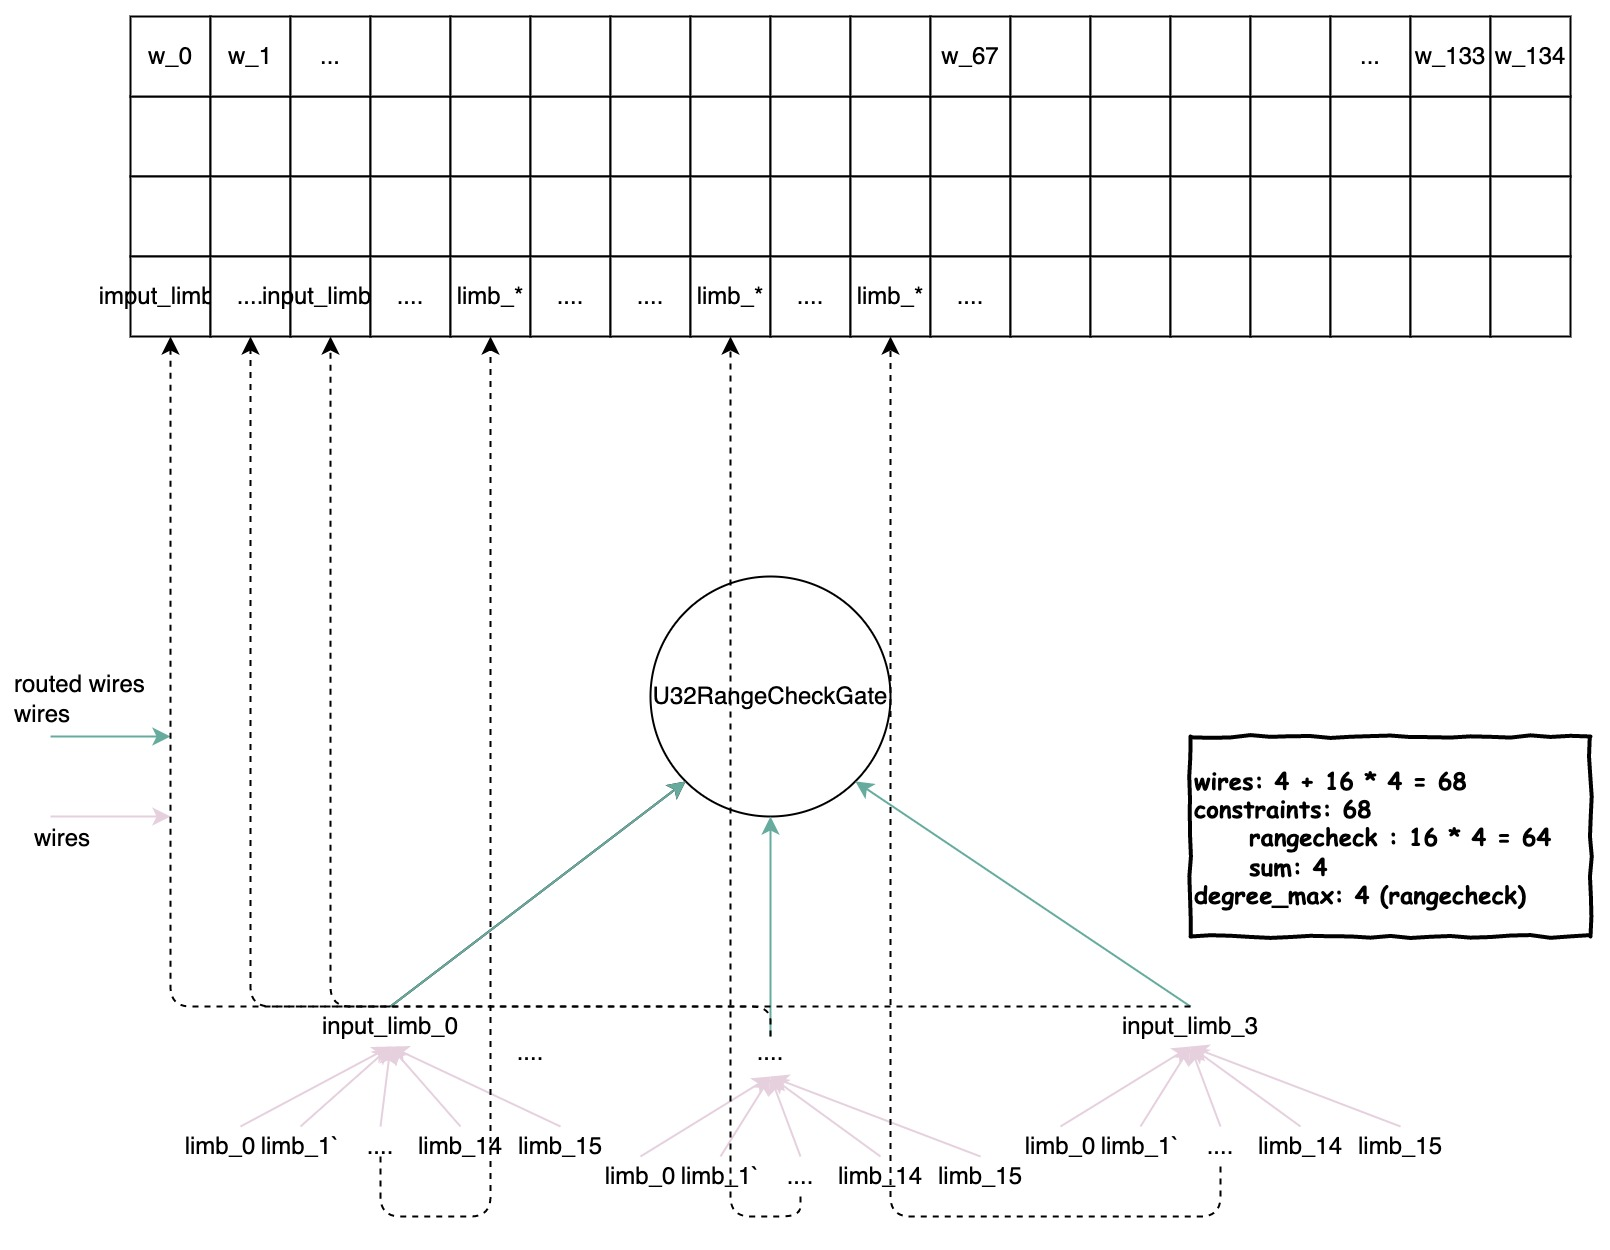
\includegraphics[width=0.6\textwidth]{gates/range_check_u32.jpeg}
    \caption{U32RangeCheckGate}
    \label{fig:range-check-u32}
\end{figure}

Constraints for each input\_limb:
\begin{itemize}
    \item Each input\_limb consists of its aux\_limbs. -- 1 constraint with degree 1.
    \begin{lstlisting}[language=rust]
let computed_sum = reduce_with_powers(&aux_limbs, base);
constraints.push(computed_sum - input_limb);
    \end{lstlisting}
    \item aux\_limbs range check. -- 16 (aux\_limbs) constraints with degree BASE ($(x-0)(x-1)\cdots(x-\text{BASE}+1)$).
\end{itemize}

In summary, there are 17 constraints per input limb, a total of $\text{num\_input\_limbs} \times 17$ constraints. 
The degree of the gate equals BASE for range check.

\subsubsubsection{subtraction\_u32}

\hspace*{\fill}

\indent U32SubtractionGate is a gate to perform subtraction on 32-bit limbs: given `x', `y', and `borrow', it returns 
the result $x - y - \text{borrow}$ and, if this underflows, a new `borrow'.

The gate structure is like \figref{fig:subtraction-u32}.

\begin{figure}[!ht]
    \centering
    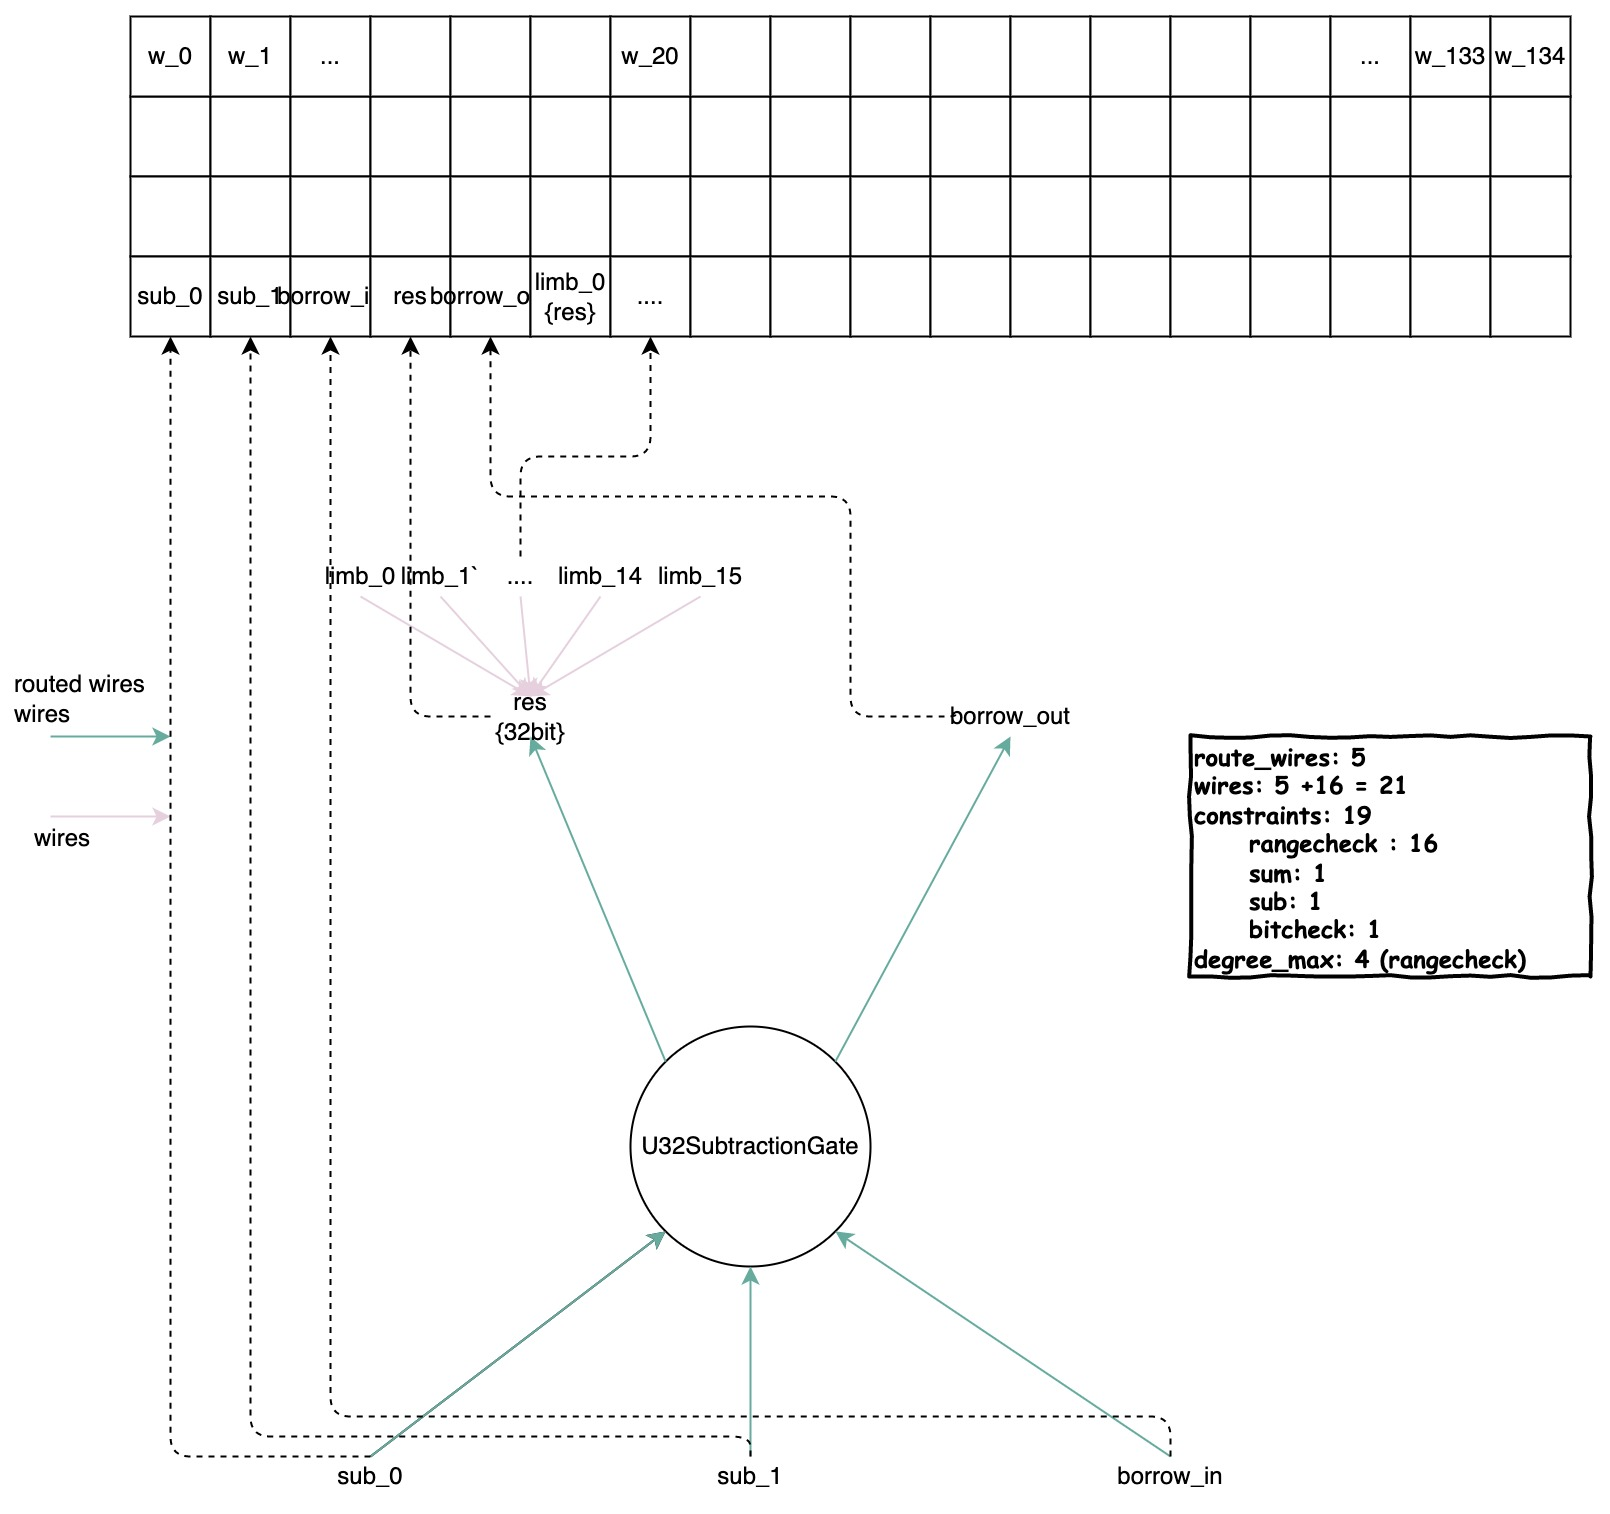
\includegraphics[width=0.6\textwidth]{gates/subtraction_u32.jpeg}
    \caption{U32SubtractionGate}
    \label{fig:subtraction-u32}
\end{figure}

Constraints for each operation:
\begin{itemize}
    \item Constrain the calculation. -- 1 constraint with degree 2.
    \begin{lstlisting}[language=rust]
let result_initial = input_x - input_y - input_borrow;
...
constraints.push(output_result - (result_initial + base * output_borrow));
    \end{lstlisting}
    \item Limbs range check. -- 16 (limbs) constraints with degree 4. (limbs are all 2-bits)
    \item Constrain limbs for res. -- 1 constraint with degree 1.
    \item Constrain borrow\_out to be one bit. -- 1 constraint with degree 1.
\end{itemize}

In summary, there are 19 constraints for each operation. The degree of the gate is 4 which is needed by the 4-bits limbs range check.

\subsubsection{Gadgets}



\subsubsubsection{biguint-add}

\begin{enumerate}
    \item \verb|Target|: Implement the addition of two biguints.
    \item \verb|Constraints logic|: 
        \begin{itemize}
            \item Equation for gates;
            \item Sumcheck between output and limbs;
            \item Rangecheck for limbs.
        \end{itemize}
    \item \verb|Circuit layout|: See \figref{fig:biguint-add-circuit-layout}.
    \item \verb|Trace layout|: See \figref{fig:biguint-add-trace-layout}.
    \item \verb|Constraints info and costs|
    \begin{itemize}
        \item gate type num: 1 (U32AddManyGate)
        \item gate ops num: limbs-num
        \item gate instance num: ceil(limbs-num / gate.ops)
        \item copy-constraints: limbs-num * 4
        \item max-degree: 4 (\verb|1 << limb-bits|)
    \end{itemize}
\end{enumerate}

\begin{figure}[!ht]
    \centering
    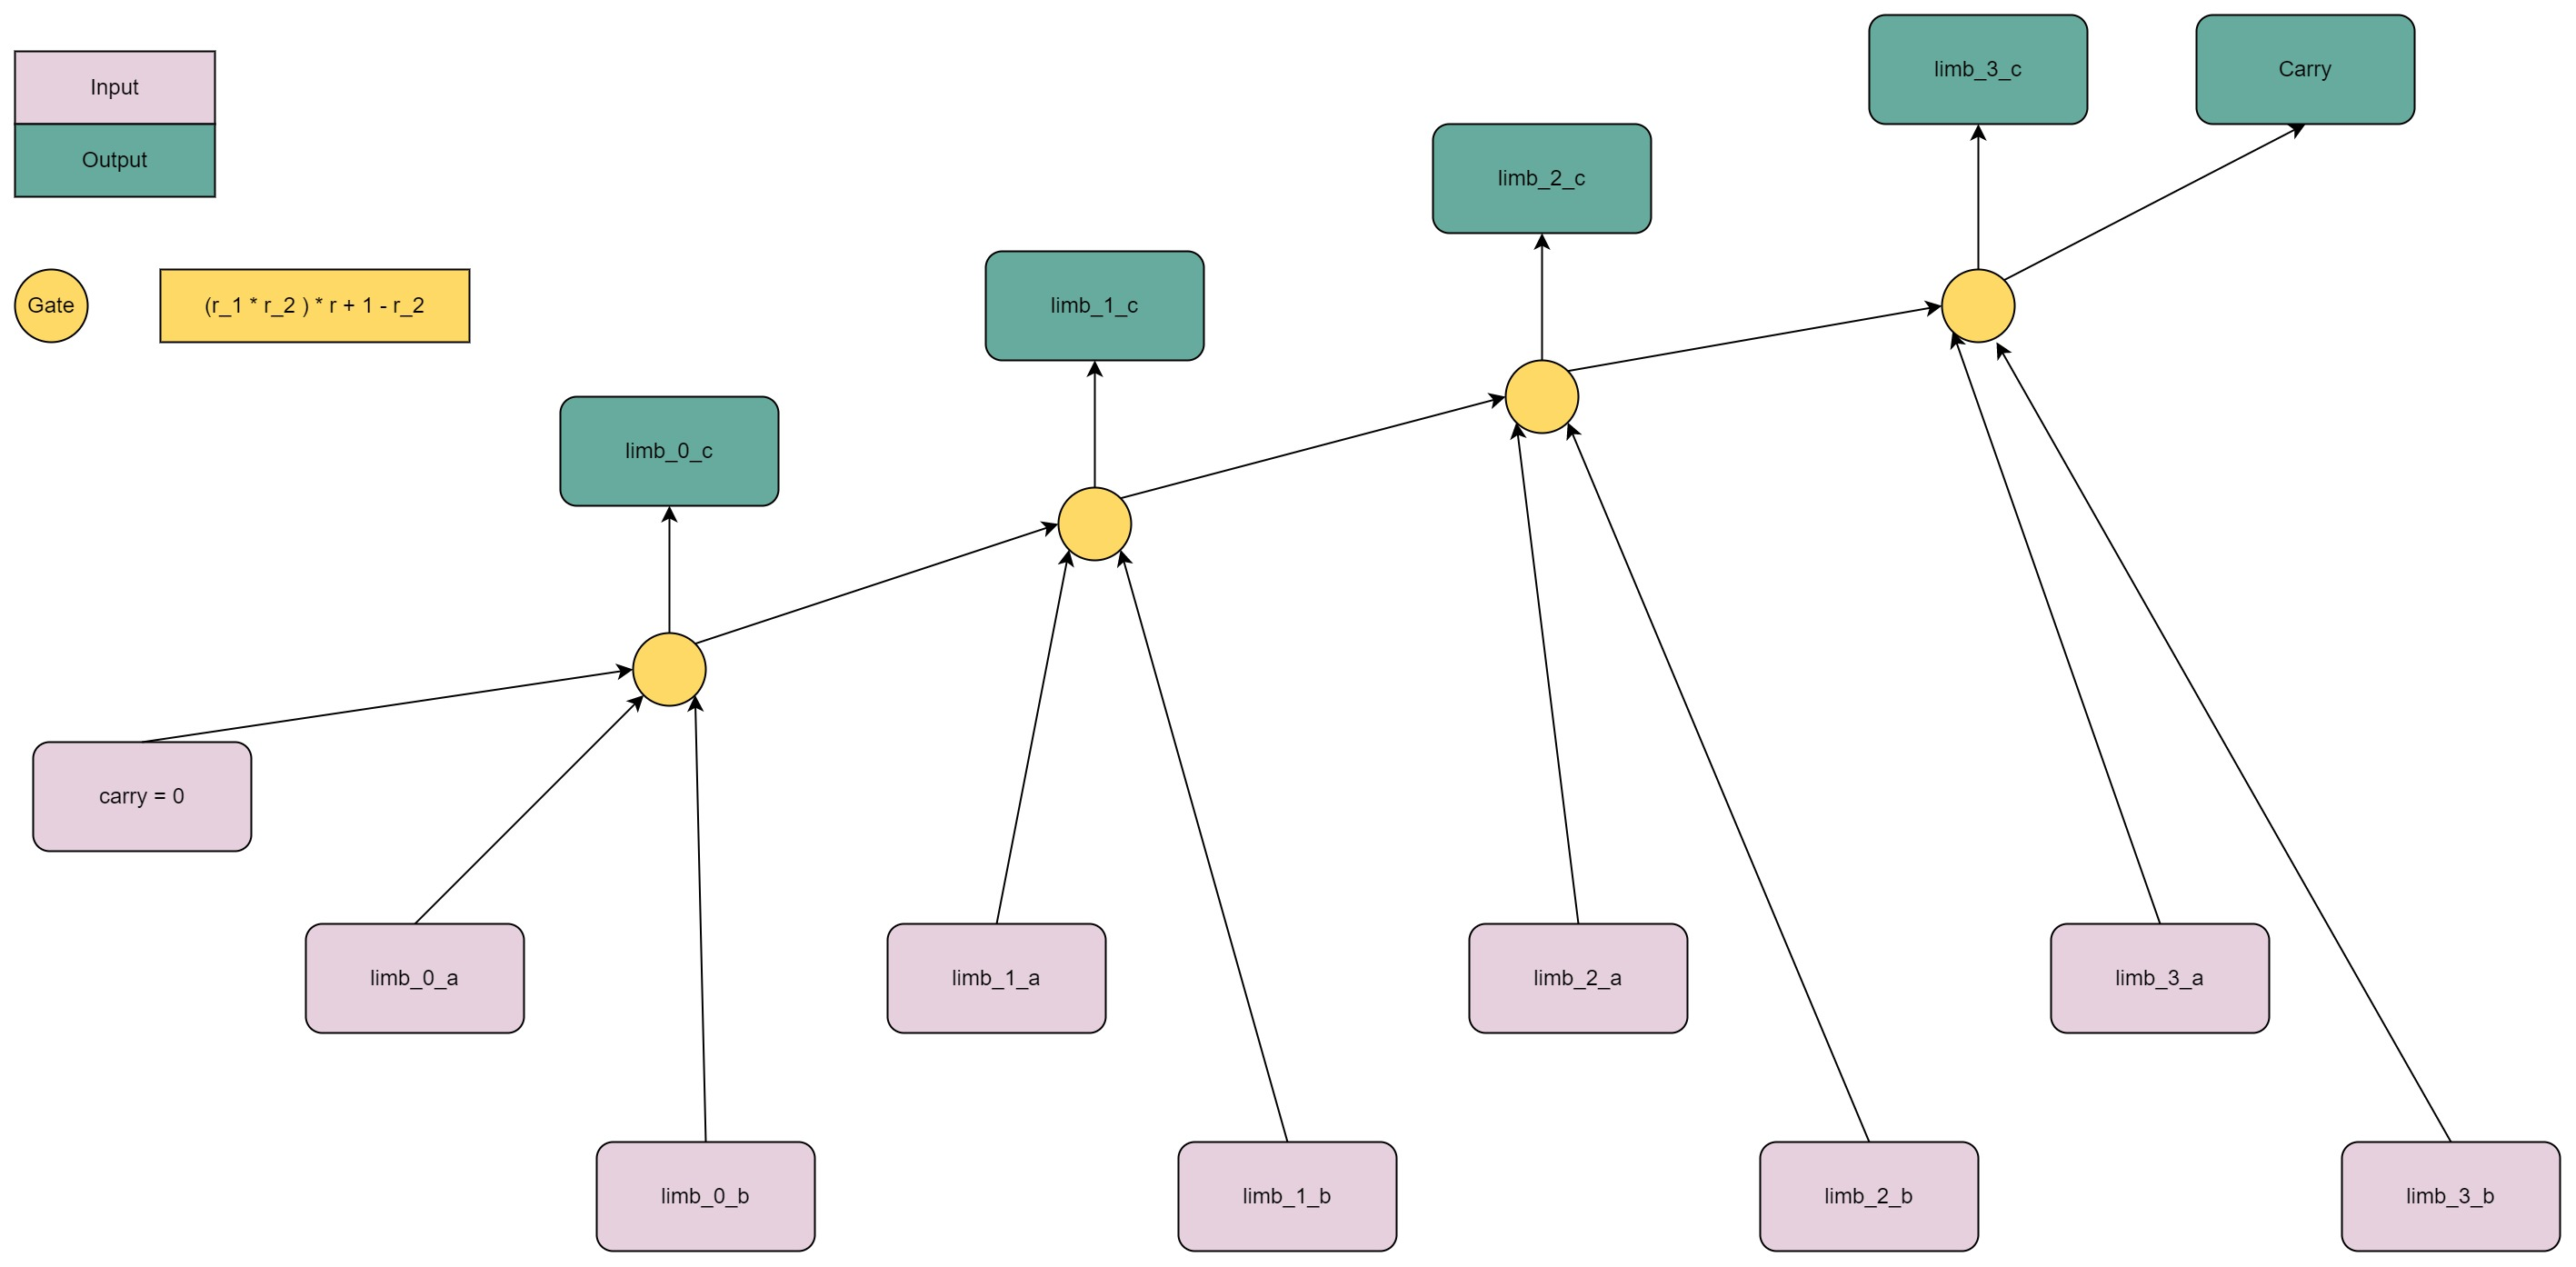
\includegraphics[width=0.6\textwidth]{biguint-add-circuit-layout.jpg}
    \caption{biguint-add circuit layout}
    \label{fig:biguint-add-circuit-layout}
\end{figure}
 
\begin{figure}[!ht]
    \centering
    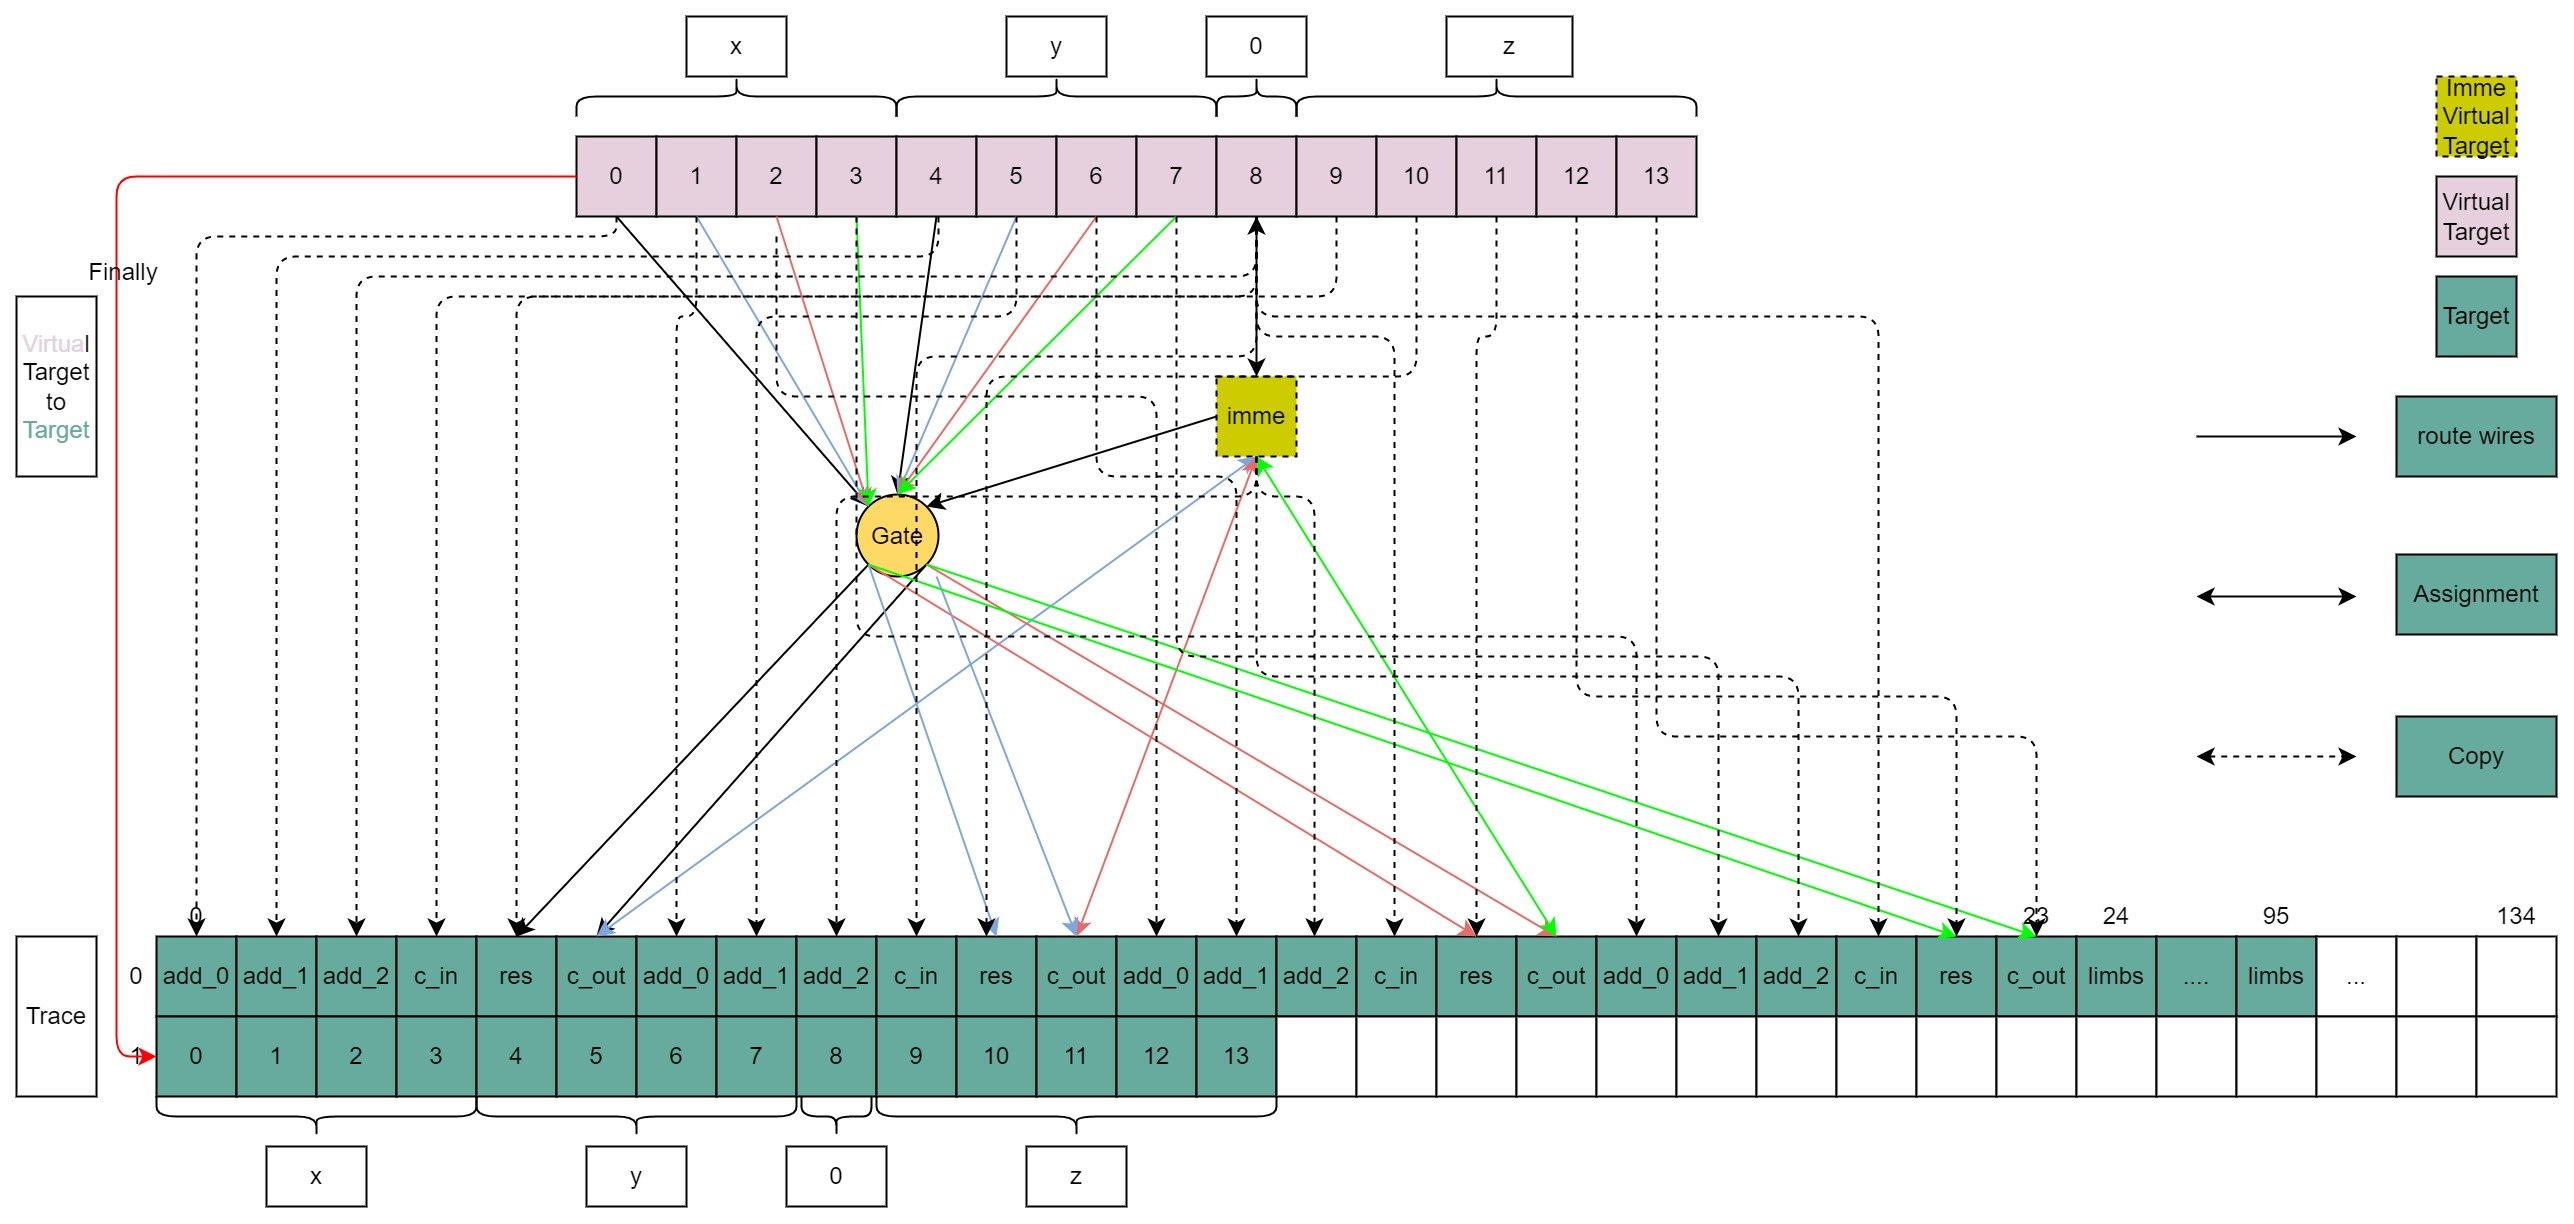
\includegraphics[width=0.6\textwidth]{biguint-add-trace-layout.jpg}
    \caption{biguint-add trace layout}
    \label{fig:biguint-add-trace-layout}
\end{figure}

\subsubsubsection{biguint-sub}

\begin{enumerate}
    \item \verb|Target|: Implement the substraction of two biguints.
    \item \verb|Constraints logic|:
    \begin{itemize}
        \item Equation for gate;
        \item Sumcheck for ouptput;
        \item Rangecheck for limbs.
    \end{itemize}
    \item \verb|Circuit layout|: See \ref{fig:biguint-sub-circuit-layout}.
    \item \verb|Trace layout|: See \ref{fig:biguint-sub-trace-layout}.
    \item \verb|Constraints info and costs|:
    \begin{itemize}
        \item constraints-num: $6 \times (3 + 32 / 2) = 114$
        \item copy-constraints: $16$
        \item max-degree: $4$
        \item wires-num: $6 \times (5 + 16) = 126$
    \end{itemize}
\end{enumerate}

\begin{figure}[!ht]
    \centering
    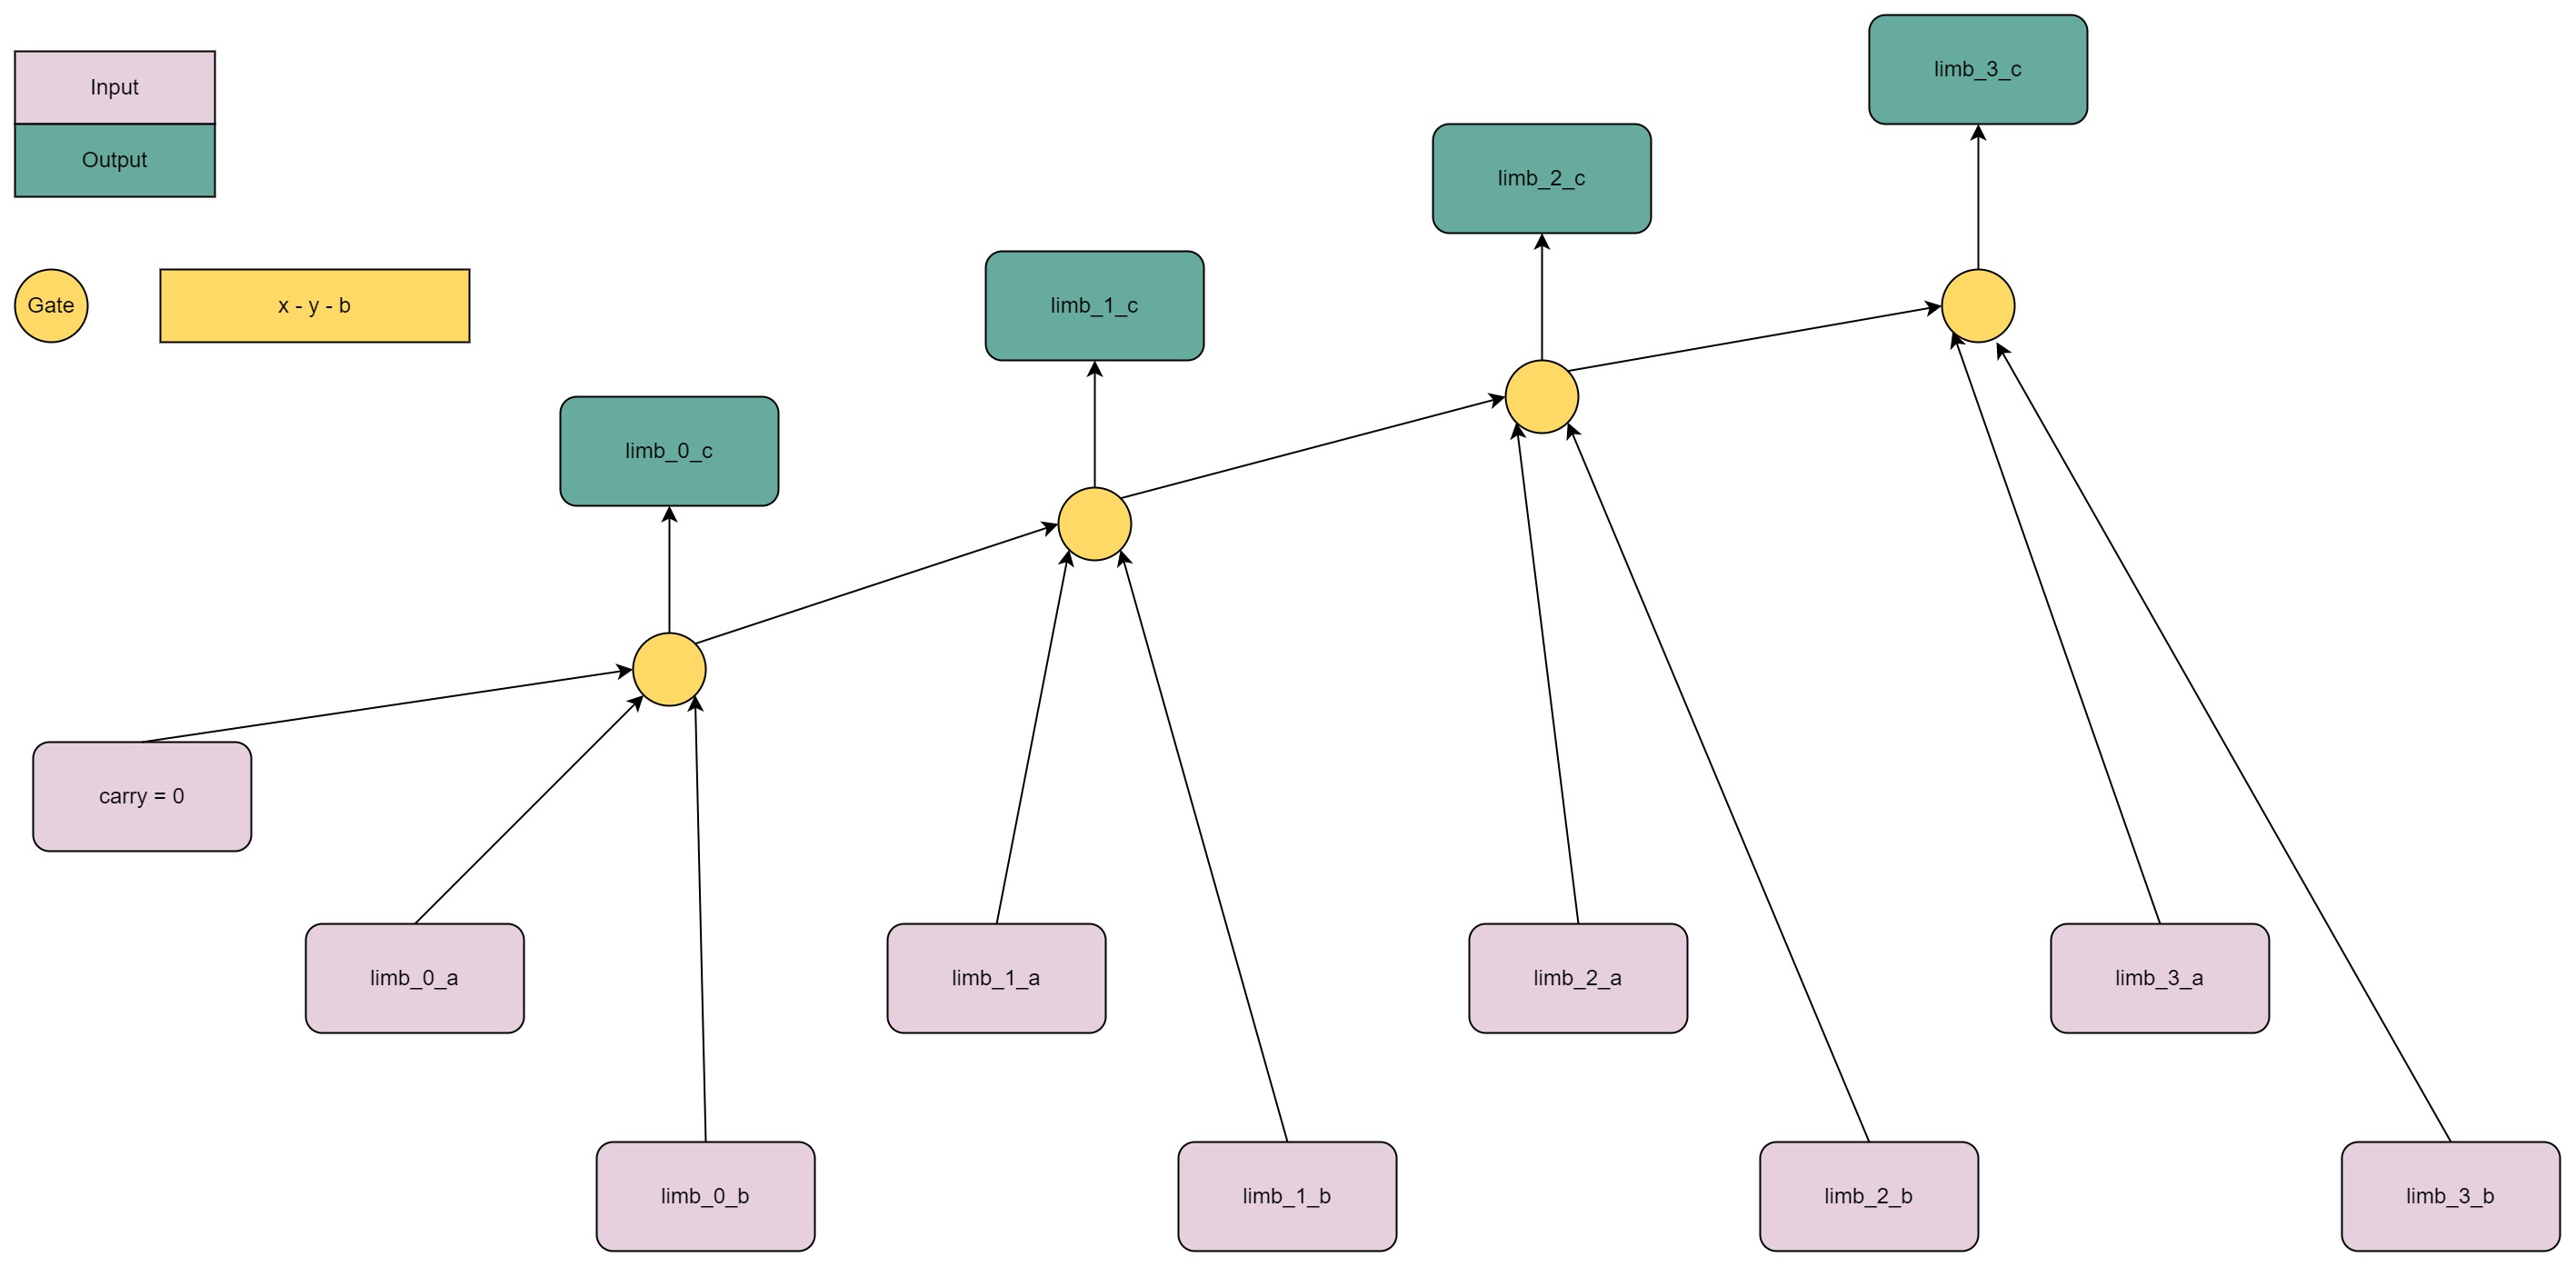
\includegraphics[width=0.6\textwidth]{biguint-sub-circuit-layout.jpg}
    \caption{biguint-sub circuit layout}
    \label{fig:biguint-sub-circuit-layout}
\end{figure}

\begin{figure}[!ht]
    \centering
    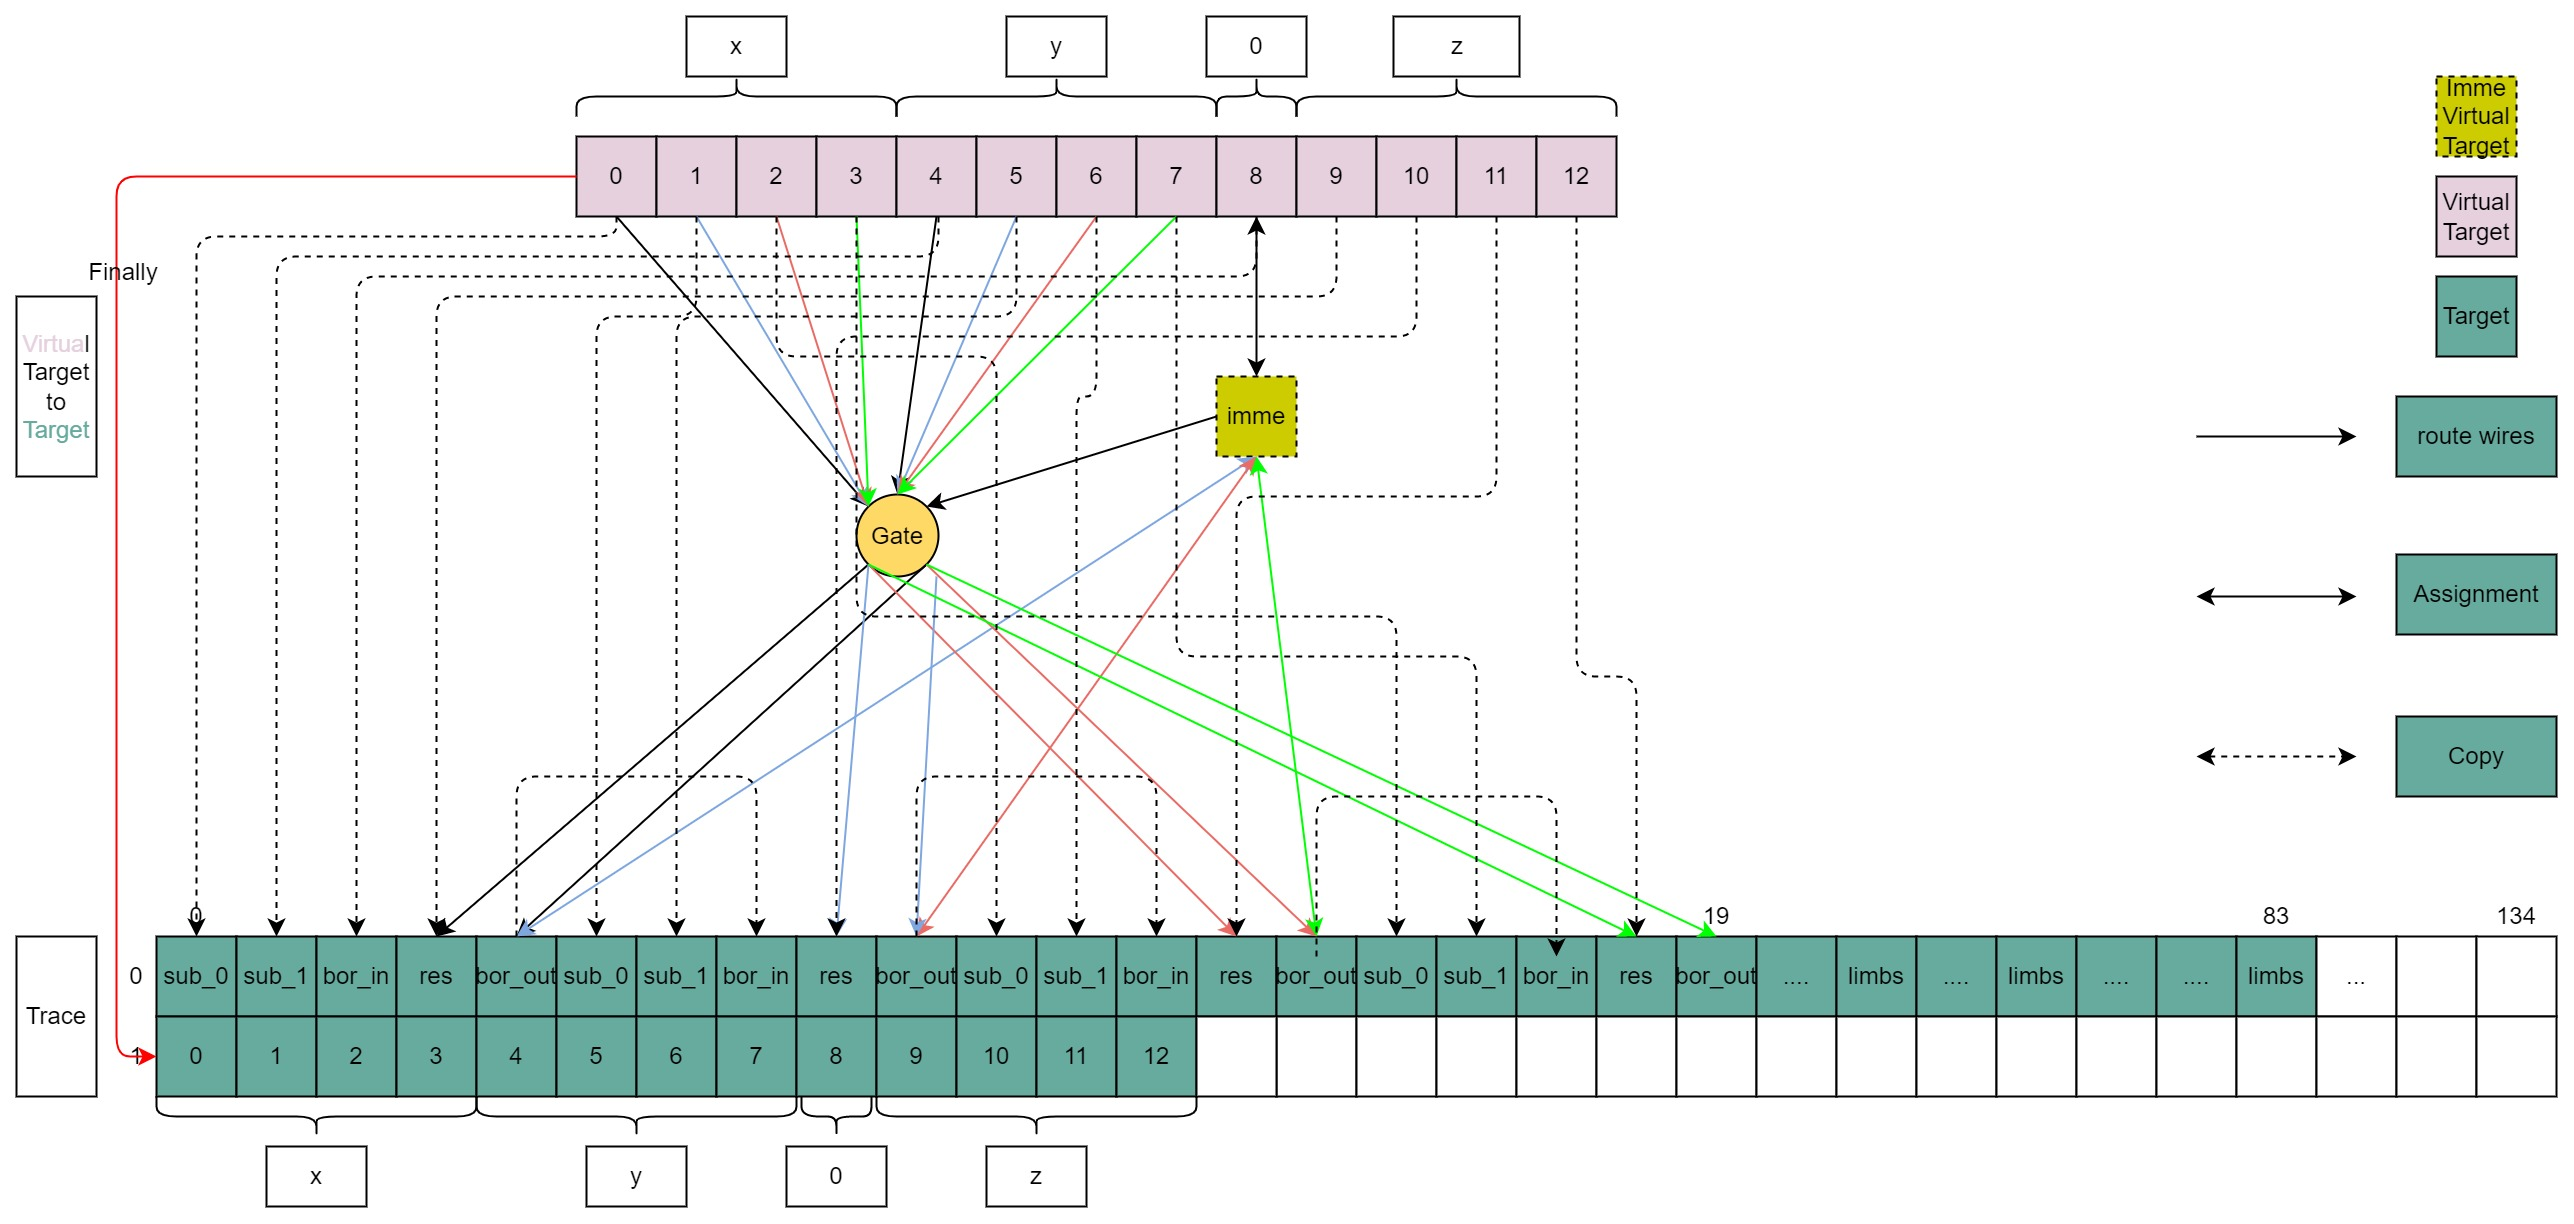
\includegraphics[width=0.6\textwidth]{biguint-sub-trace-layout.jpg}
    \caption{biguint-sub trace layout}
    \label{fig:biguint-sub-trace-layout}
\end{figure}
\paragraph{biguint-mul}

\begin{enumerate}
    \item \verb|Target|: Implement the multiplication of two biguints.
    \item \verb|Constraints logic|:
    \begin{itemize}
        \item Compute mul-factors first, use U32ArithmeticGate;
        \item Add mul-factors from low bits, use U32AddManyGate.
    \end{itemize}
    \item \verb|Process layout|: See \figref{fig:biguint-mul-layout}
    \item \verb|Constraints info and costs|:
    \begin{itemize}
        \item Gate type num: 4 (U32ArithmeticGate, U32AddManyGate(num-addends: 4), U32AddManyGate(num-addends: 6), U32AddManyGate(num-addends: 8))
        \item Gate instance num: 9
        \item U32ArithmeticGate num: 6
        \item U32AddManyGate num: 3
        \item copy-constraints: $18 \times 3 + (4 + 6 + 8) \times 2 + 9 = 99$
        \item max-degree: 4
    \end{itemize}
\end{enumerate}

\begin{figure}[!ht]
    \centering
    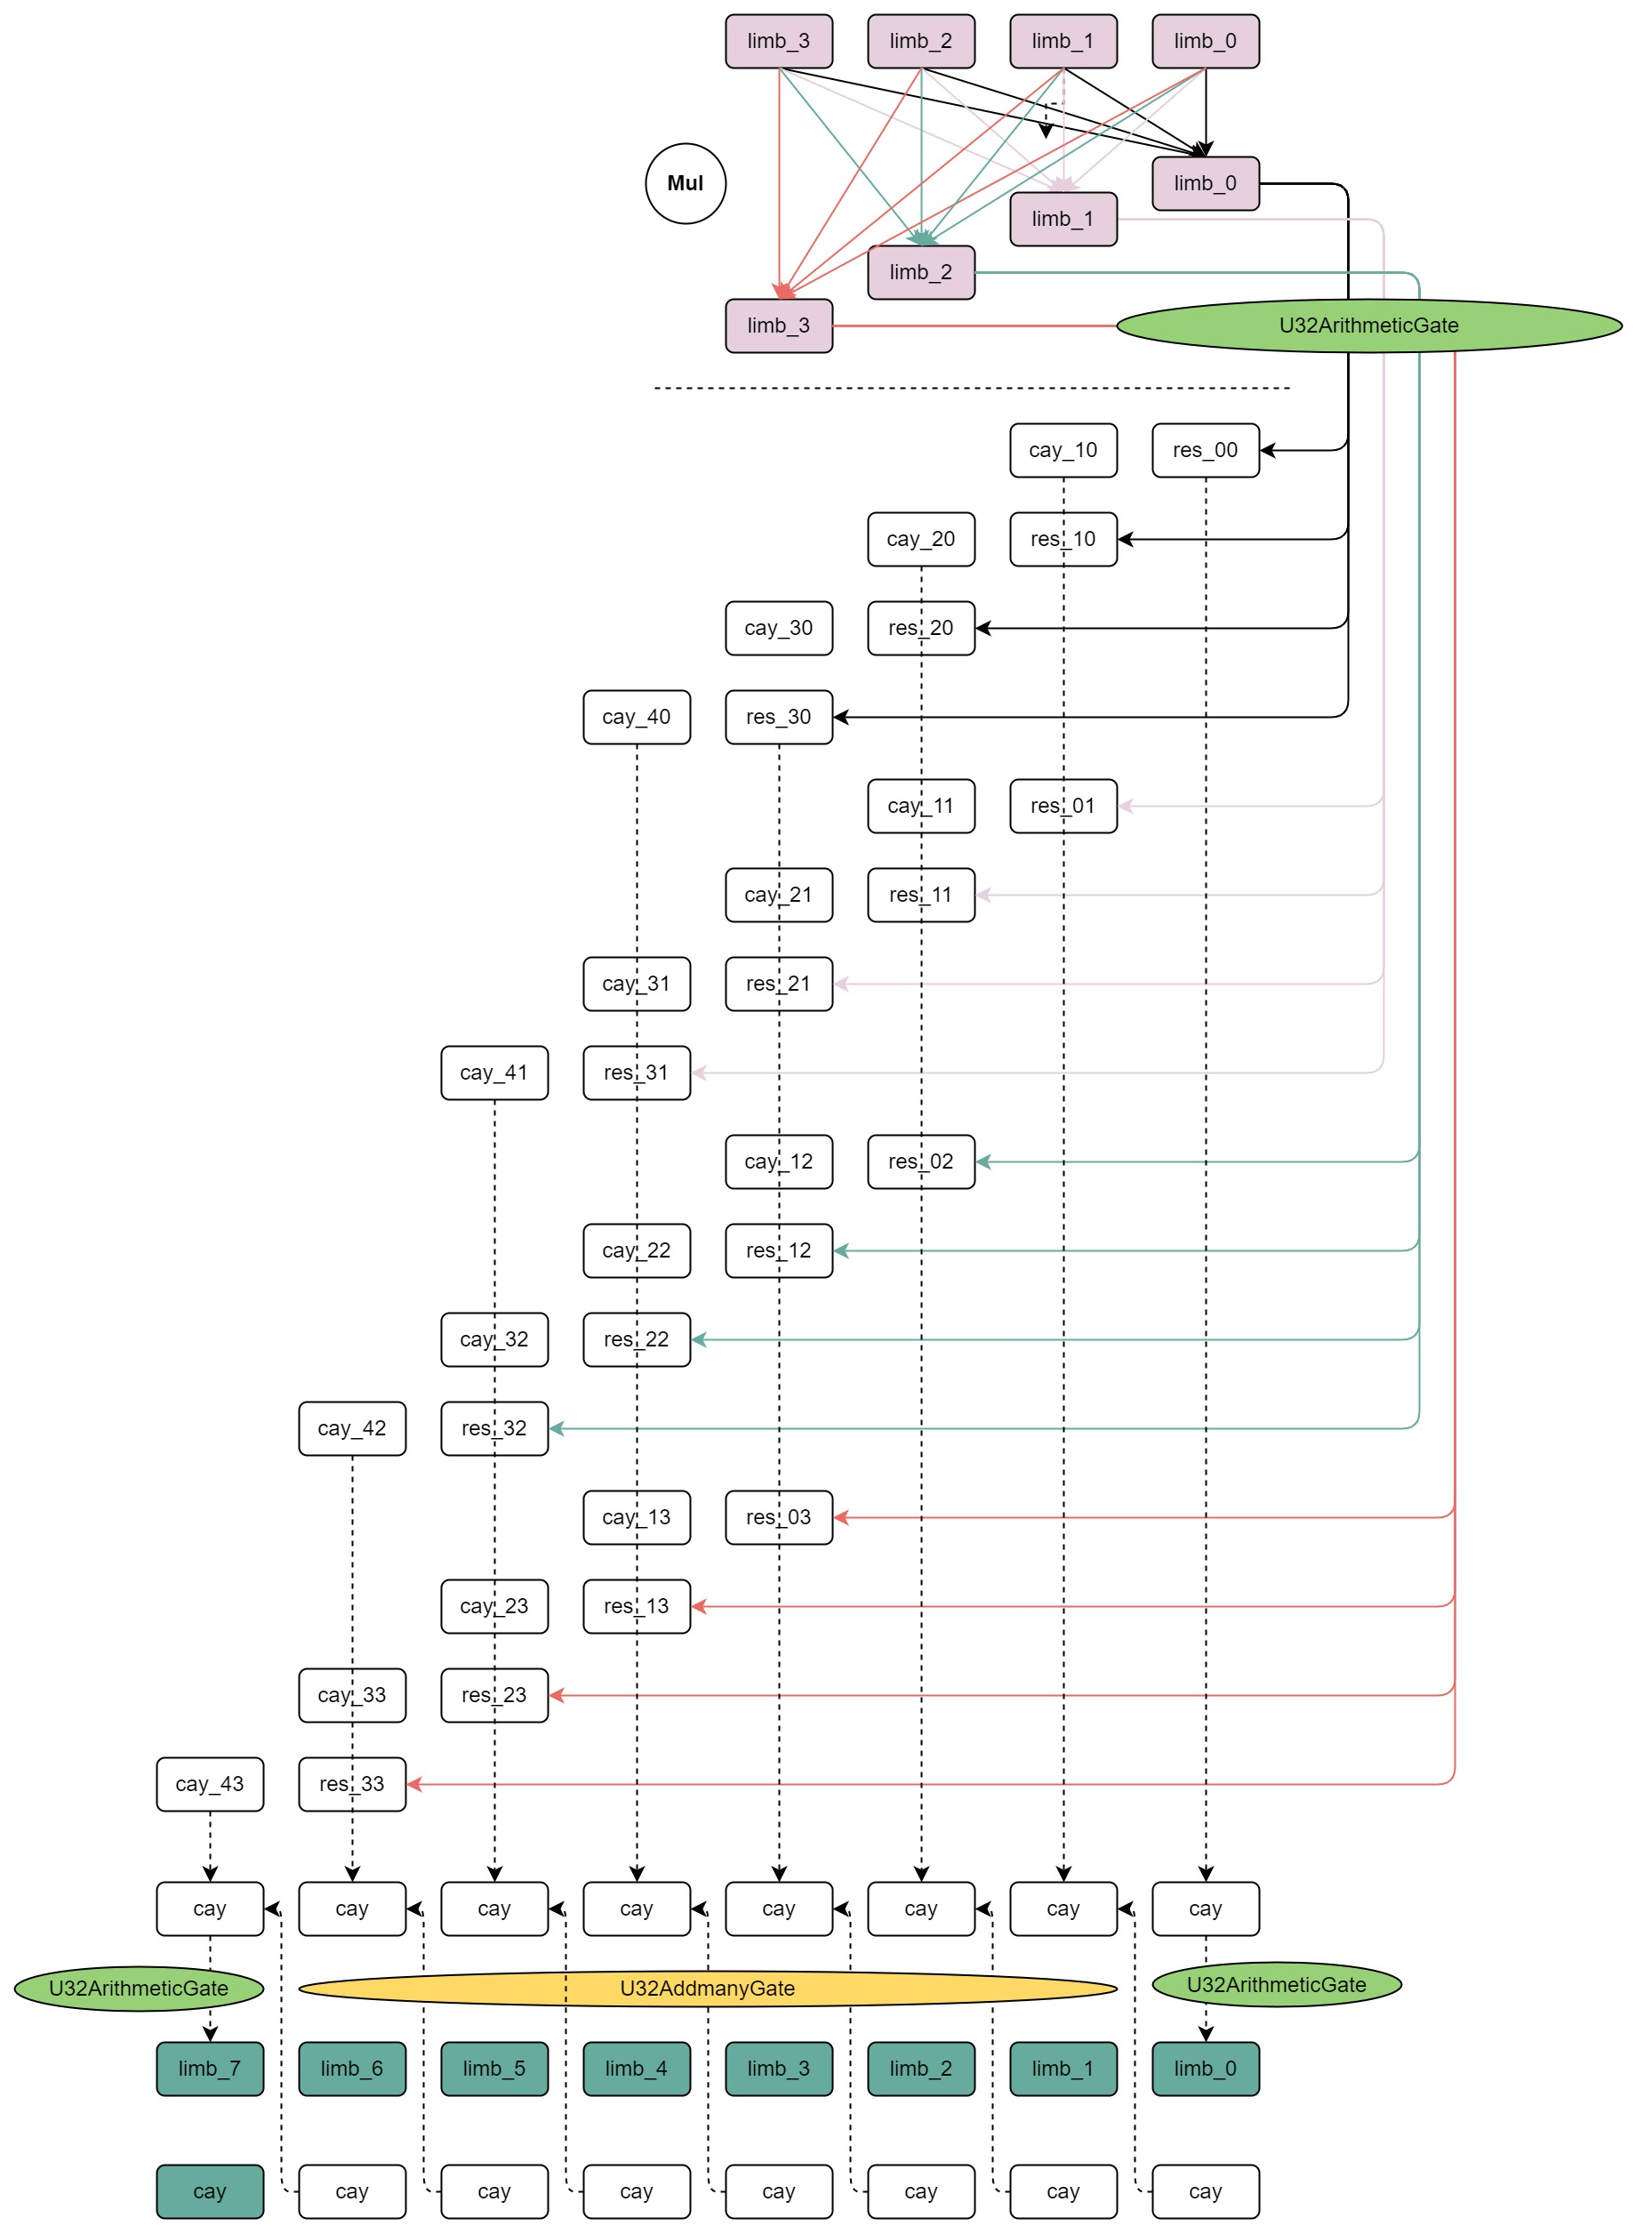
\includegraphics[width=0.6\textwidth]{biguint-mul-layout.jpg}
    \caption{biguint-mul layout}
    \label{fig:biguint-mul-layout}
\end{figure}
\paragraph{biguint-div}

Note that div-rem has the same constraints logic with div

\subparagraph{Target}
Implement the division of two biguints.

\subparagraph{Constraints logic}
\begin{itemize}
    \item Not implement div-algrithem directly;
    \item Use nondeterministic feature to check div-logic;
    \item Check \verb|div * b + rem = a|;
    \item Check \verb|rem < b|.
\end{itemize}

\subparagraph{Process layout}
See \figref{fig:biguint-div-layout}.
\begin{figure}[!ht]
    \centering
    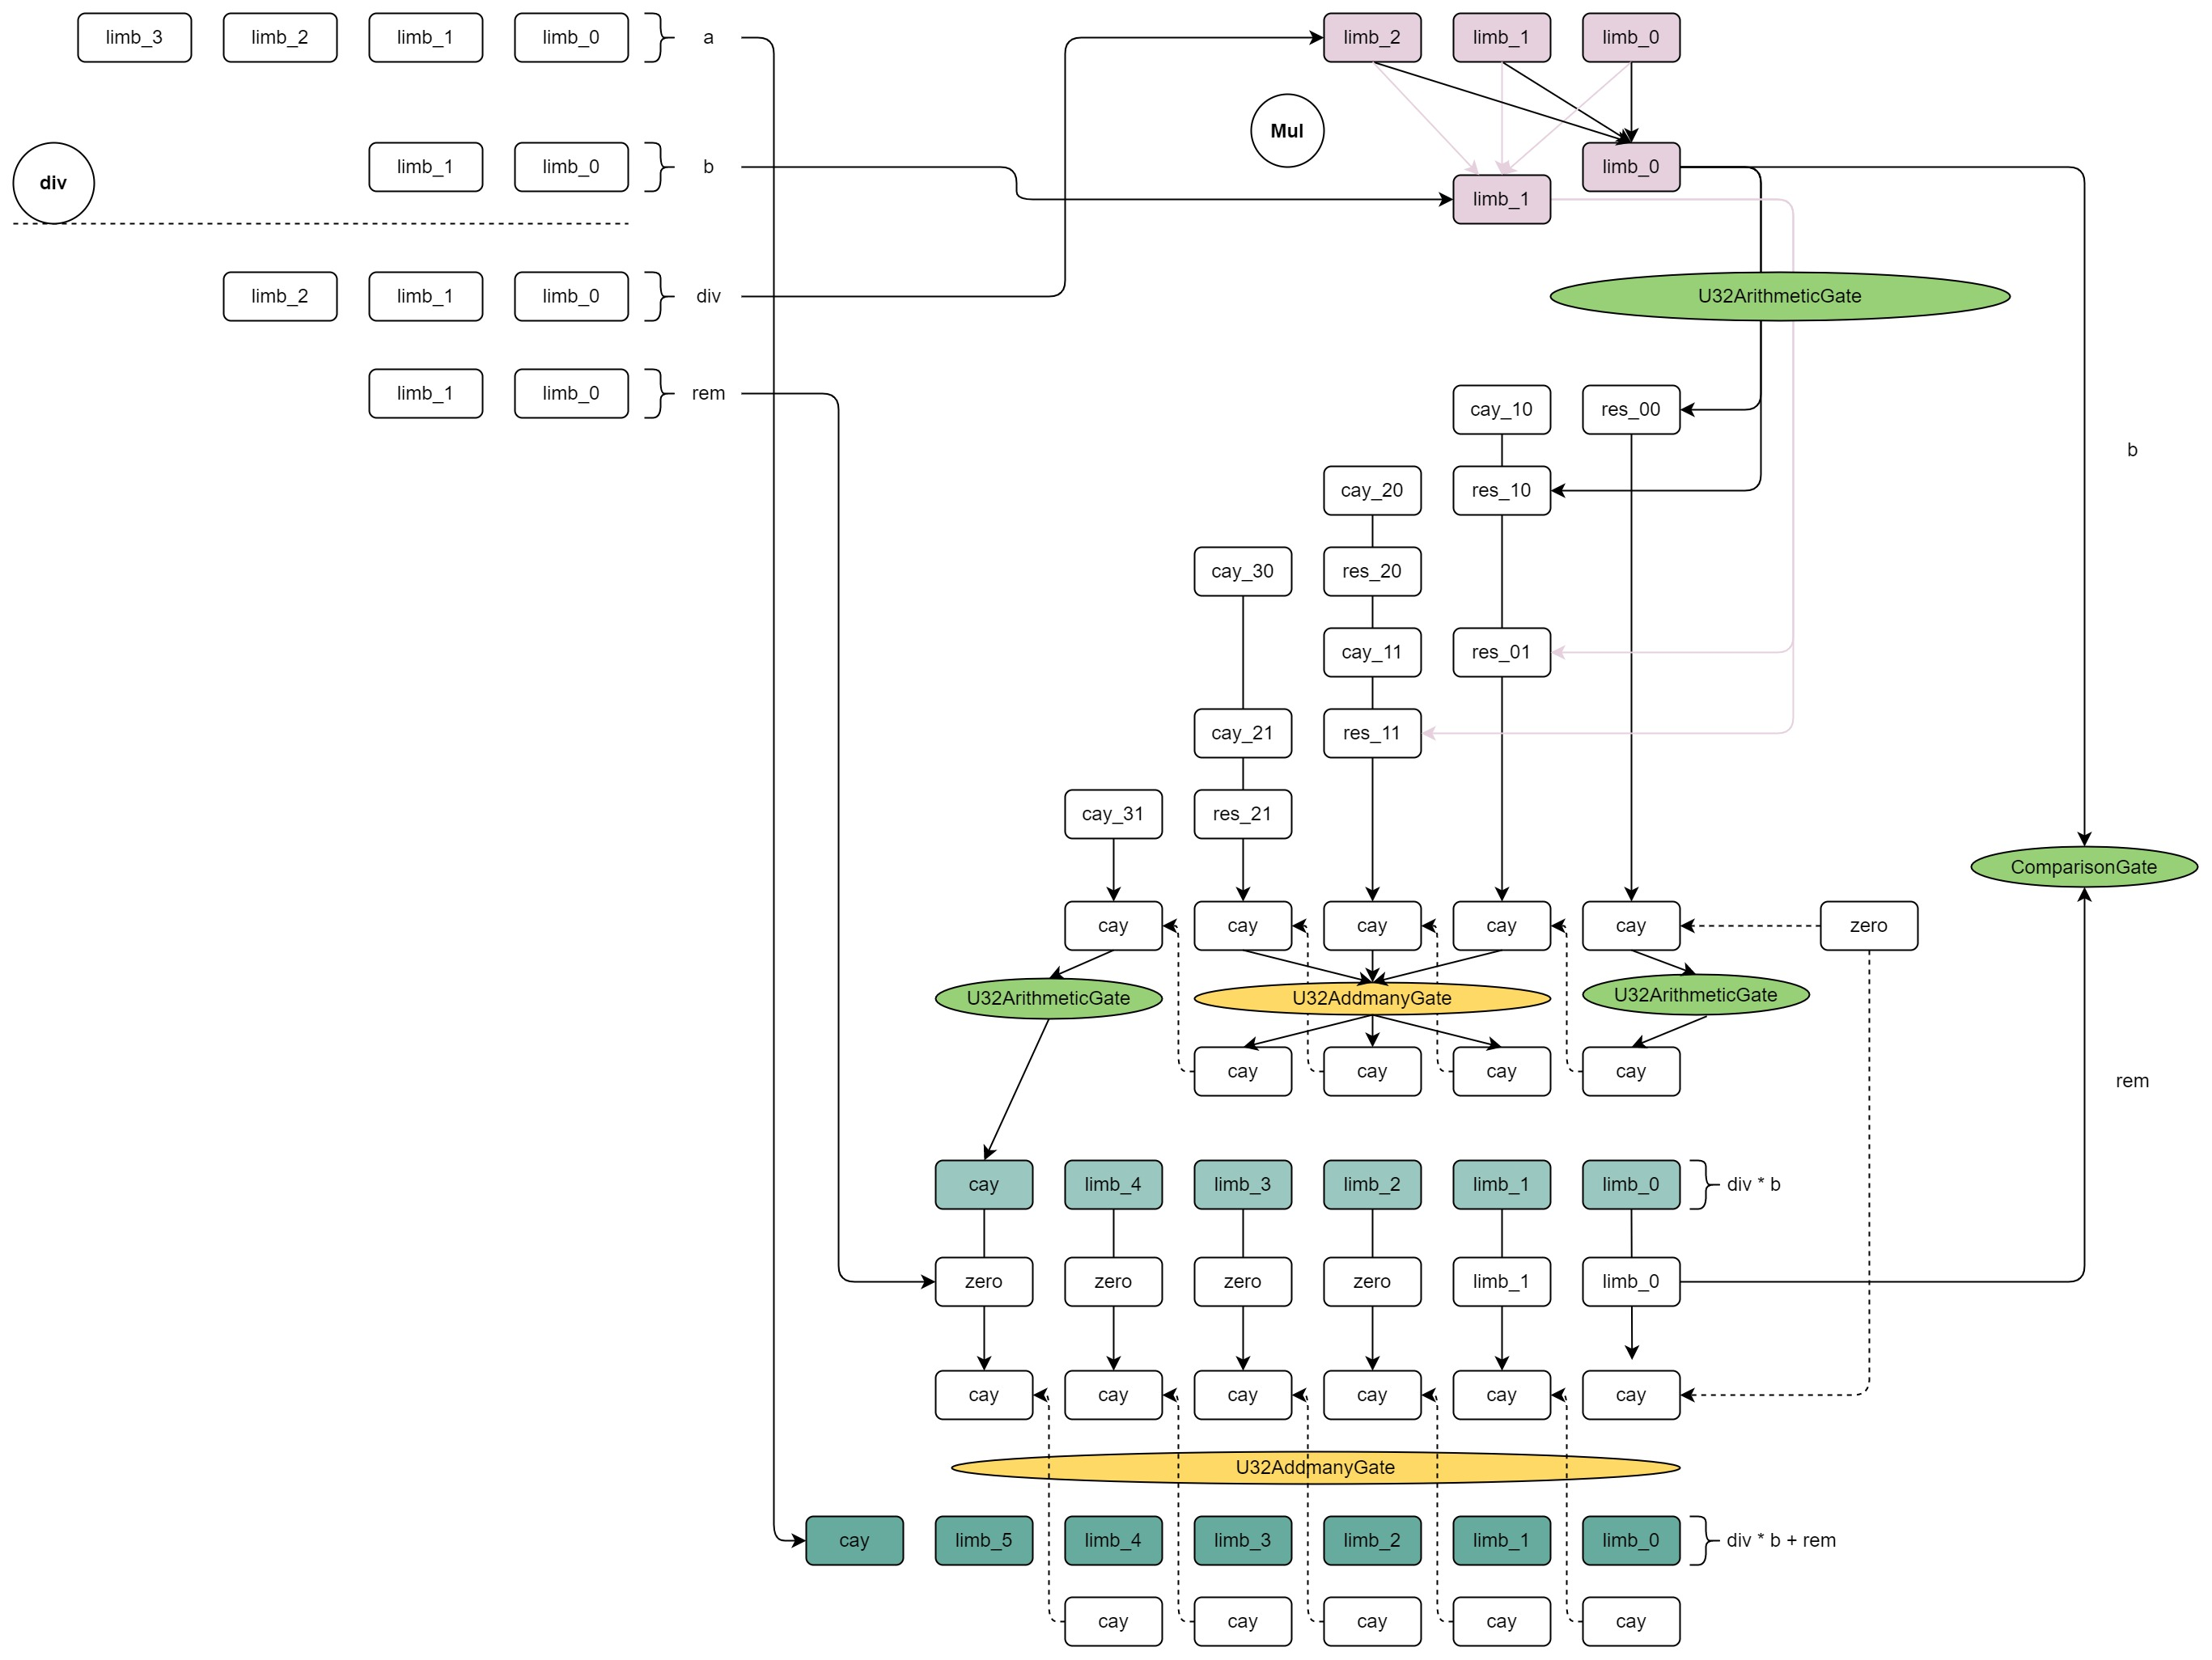
\includegraphics[width=0.8\textwidth]{biguint-div-layout.jpg}
    \caption{biguint-div layout}
    \label{fig:biguint-div-layout}
\end{figure}

\subparagraph{Constraints info and costs}
\begin{itemize}
    \item Gate type num: 5 (U32ArithmeticGate, U32AddManyGate(num-addends: 3), U32AddManyGate(num-addends: 4), ComparisionGate, ArithmeticGate)
    \item Gate instance num: $3 + 3 + 4 + 3 = 13$
    \item U32ArithmeticGate num: 3
    \item U32AddManyGate num: 3
    \item ComparisionGate num: 4
    \item ArithmeticGate num: 3
    \item copy-constraints: $3 \times 8 + 4 + 5 + 4 + 4 \times 6 + 7 + 1 + 26 + 5 = 100$
    \item max-degree: 4
\end{itemize}

\subsubsubsection{biguint-cmp}
{biguint-cmp}

\begin{enumerate}
    \item \verb|Target|: Implement the comparison of two biguints.
    \item \verb|Constraints logic|
    \begin{itemize}
        \item Split the input to many limbs, such that: \verb|limbs_num = bits / chunks|;
        \item Execute comparison for low bits limbs;
        \item Ensure that the result is determined by the highest limbs which are not equal.
    \end{itemize}
    \item \verb|Process layout|: See \ref{fig:biguint-cmp-layout}.
    \item \verb|Circuit layout|: See \ref{fig:biguint-cmp-circuit-layout}.
    \item \verb|Constraints info and costs|:
    \begin{itemize}
        \item Gate type num: 2 (ComparisionGate, ArithmeticGate)
        \item Gate instance num: $4 \times 2 + 3 = 11$
        \item ComparisionGate num: 8
        \item ArithmeticGate num: 3
        \item copy-constraints: $(4 + 9) \times 4 + 1 = 53$
        \item max-degree: 4
    \end{itemize}
\end{enumerate}

\begin{figure}[!ht]
    \centering
    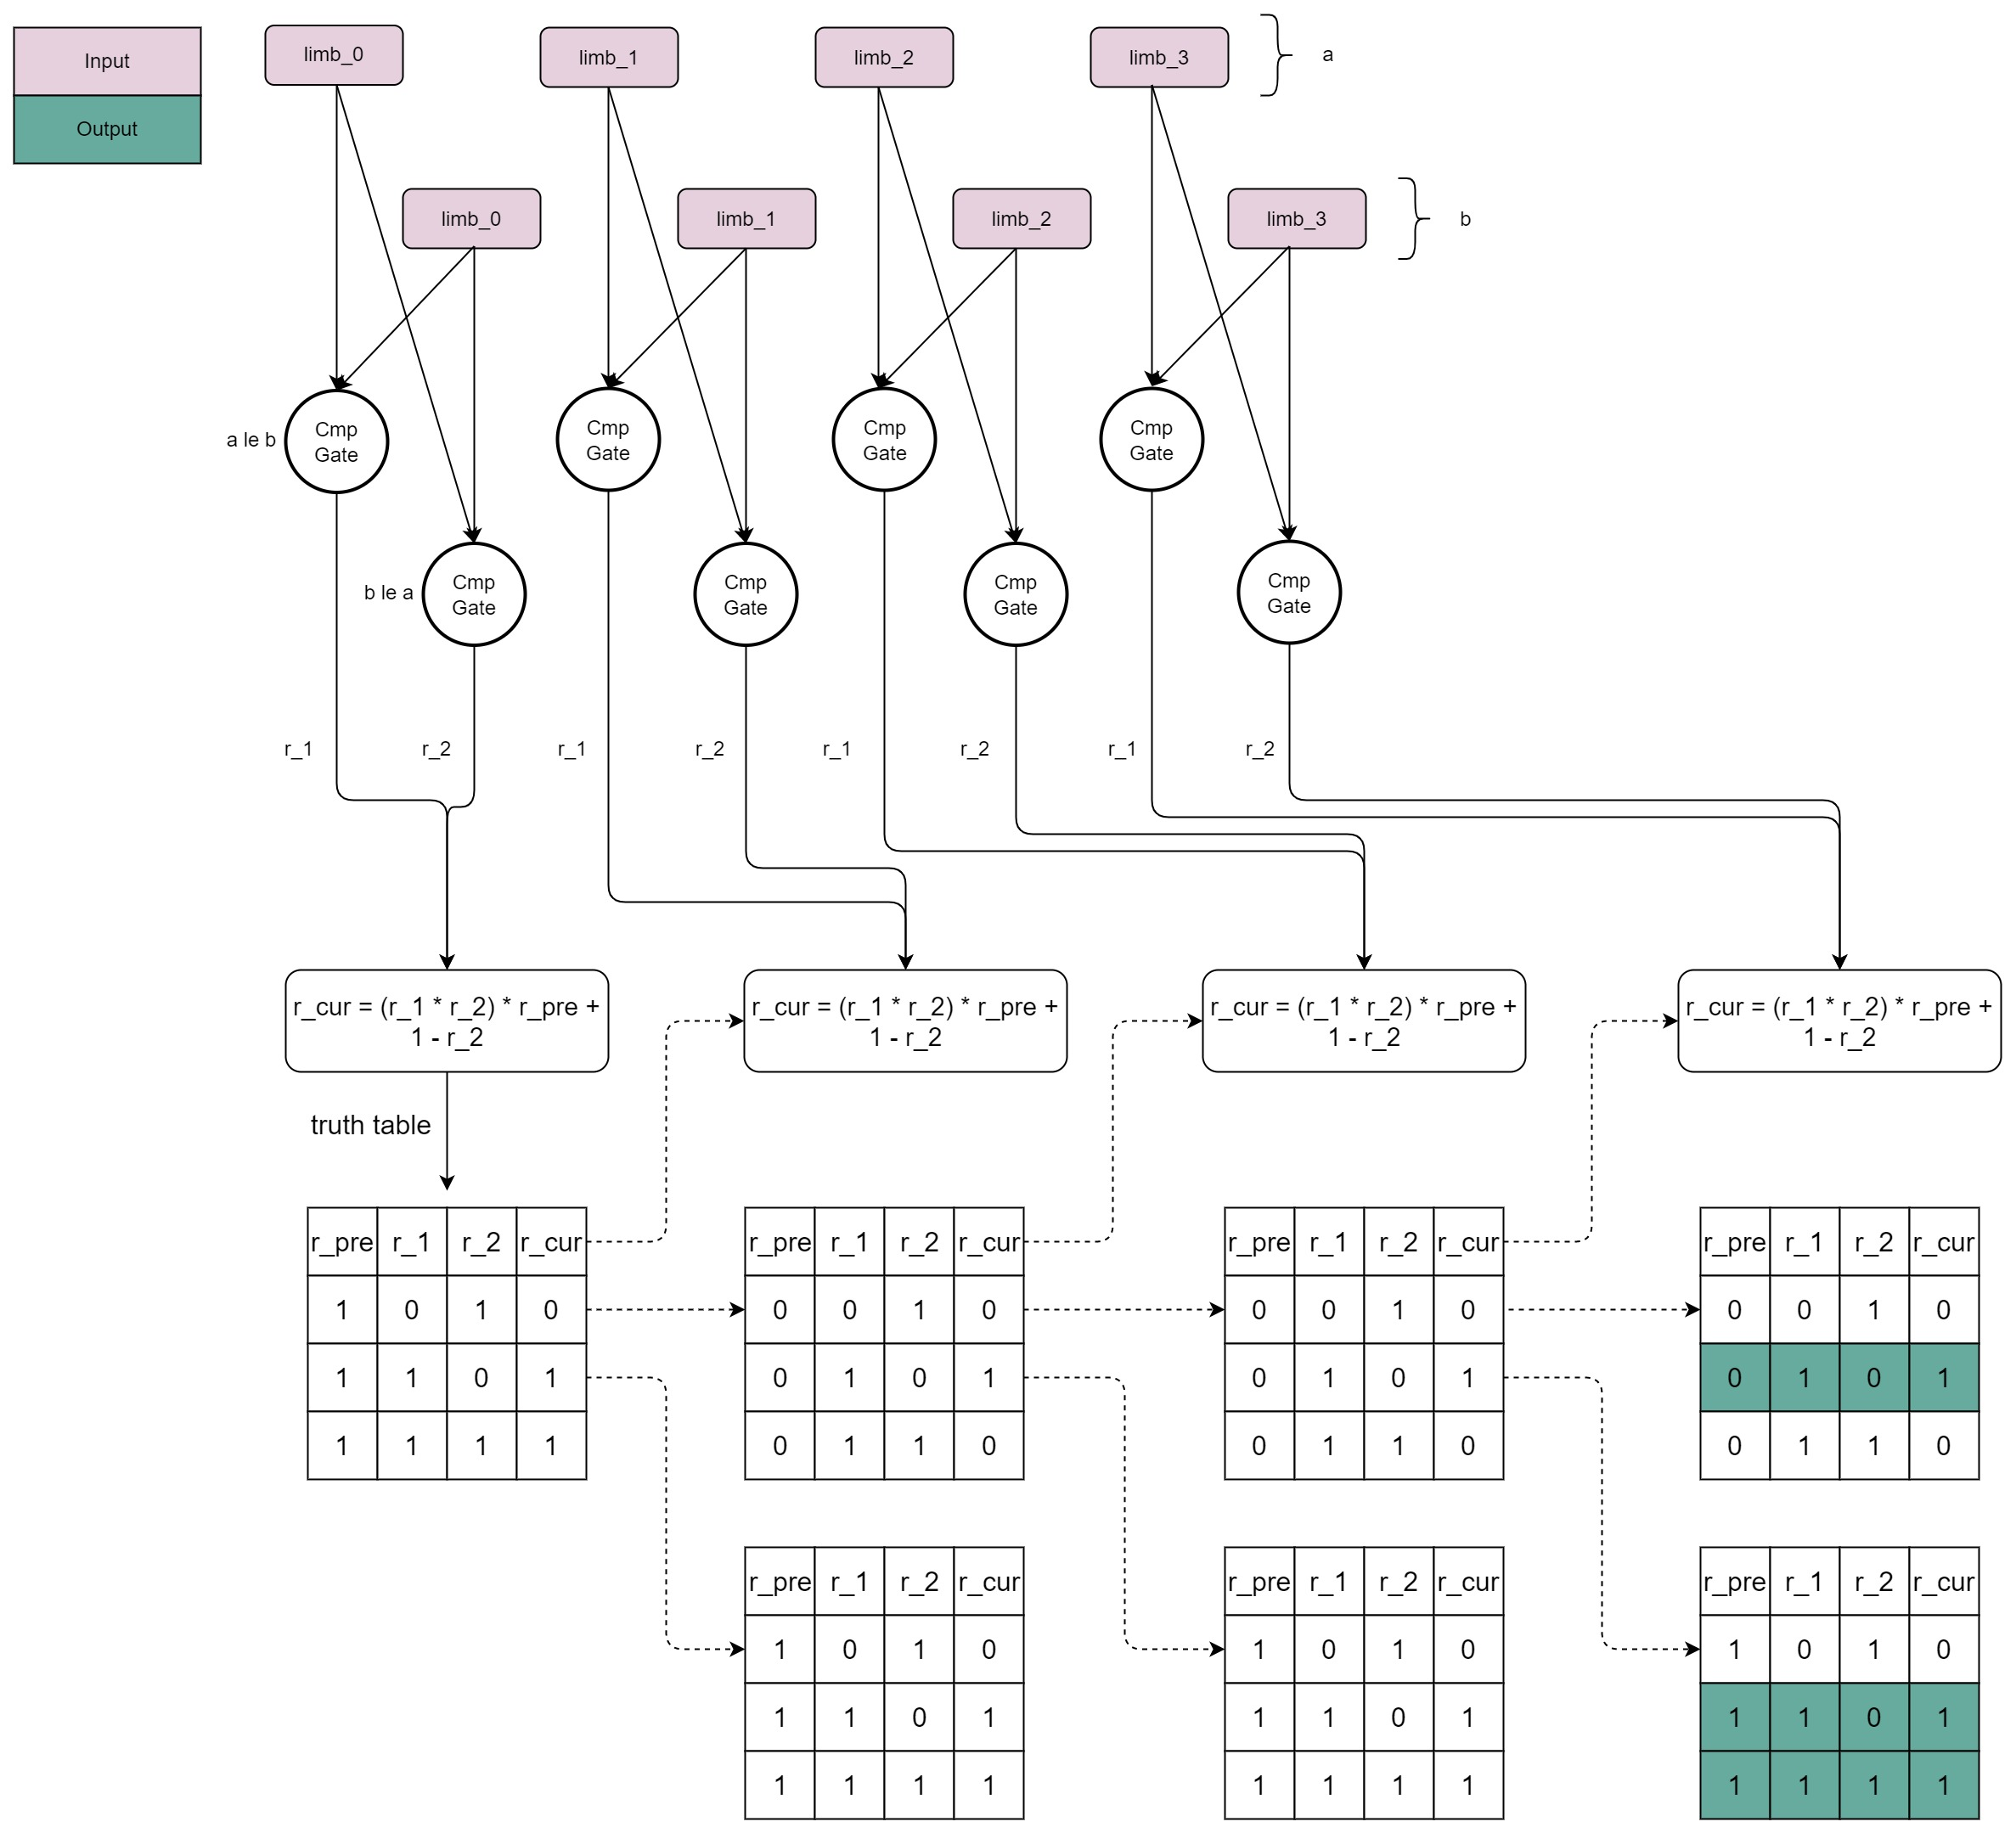
\includegraphics[width=0.6\textwidth]{biguint-cmp-layout.jpg}
    \caption{biguint-cmp layout}
    \label{fig:biguint-cmp-layout}
\end{figure}

\begin{figure}[!ht]
    \centering
    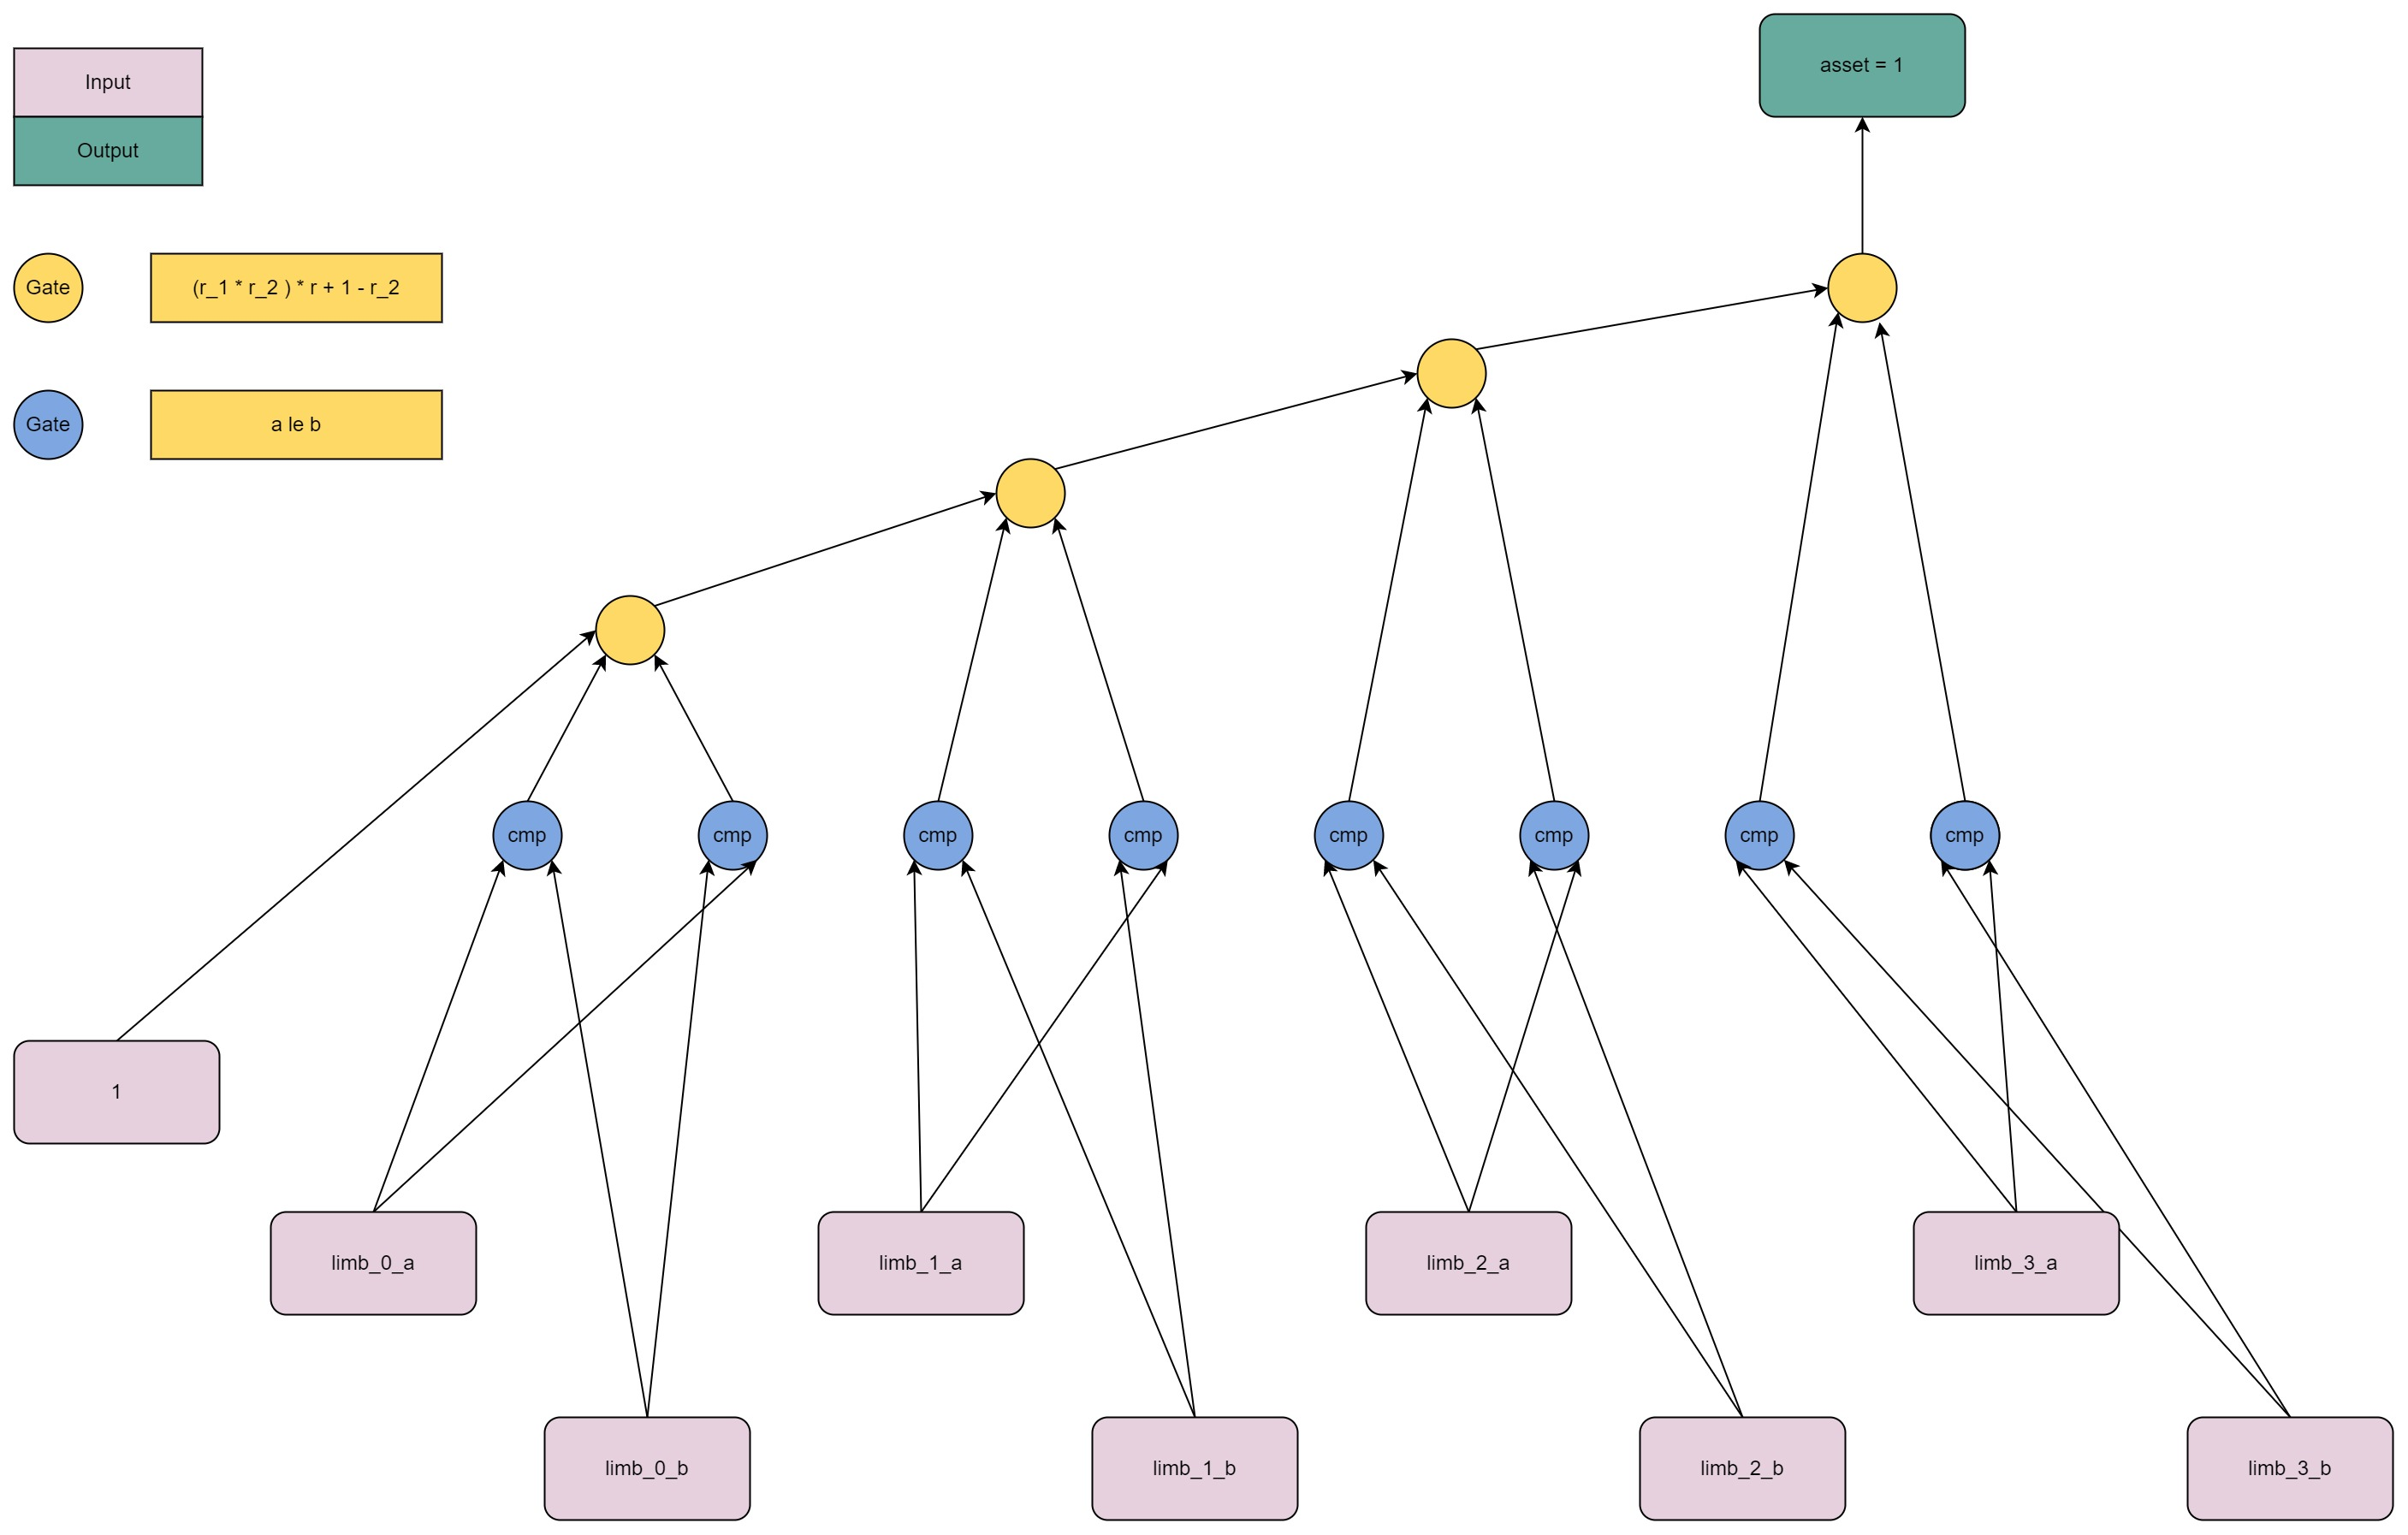
\includegraphics[width=0.6\textwidth]{biguint-cmp-circuit-layout.jpg}
    \caption{biguint-cmp circuit layout}
    \label{fig:biguint-cmp-circuit-layout}
\end{figure}

\subsubsubsection{non-native-add}

\begin{enumerate}
    \item \verb|Target|: Check the additional relation among three non-native target objects.
    \item \verb|Constraints logic|:
    \begin{itemize}
        \item Check equation for gadget: \verb|a + b = c + modular * overflow|;
        \item Check that ``c < modular''.
    \end{itemize}
    \item \verb|Process layout|: See \figref{fig:non-native-add-layout}.
    \item \verb|Constraints info and costs|:
    \begin{itemize}
        \item gadget biguint-add num: 2
        \item gadget biguint-mul-by-bool num: 1
        \item gadget biguint-cmp num: 1
        \item gate type num: 3 (U32AddManyGate, ComparisonGate, ArithmeticGate)
        \item gate instance num: 23 = 3 (U32AddManyGate) + 16 (ComparisonGate) + 2 (ArithmeticGate (1,0)) + 1 (ArithmeticGate(1,-1)) + 1 (ArithmeticGate(1,1))
        \item copy-constraints: 186 = 32 * 2{biguint-add} + 9{biguint-mul-by-bool} + 9 + (4 + 9) * 8{biguint-cmp} = 186
    \end{itemize}
\end{enumerate}

\begin{figure}[!ht]
    \centering
    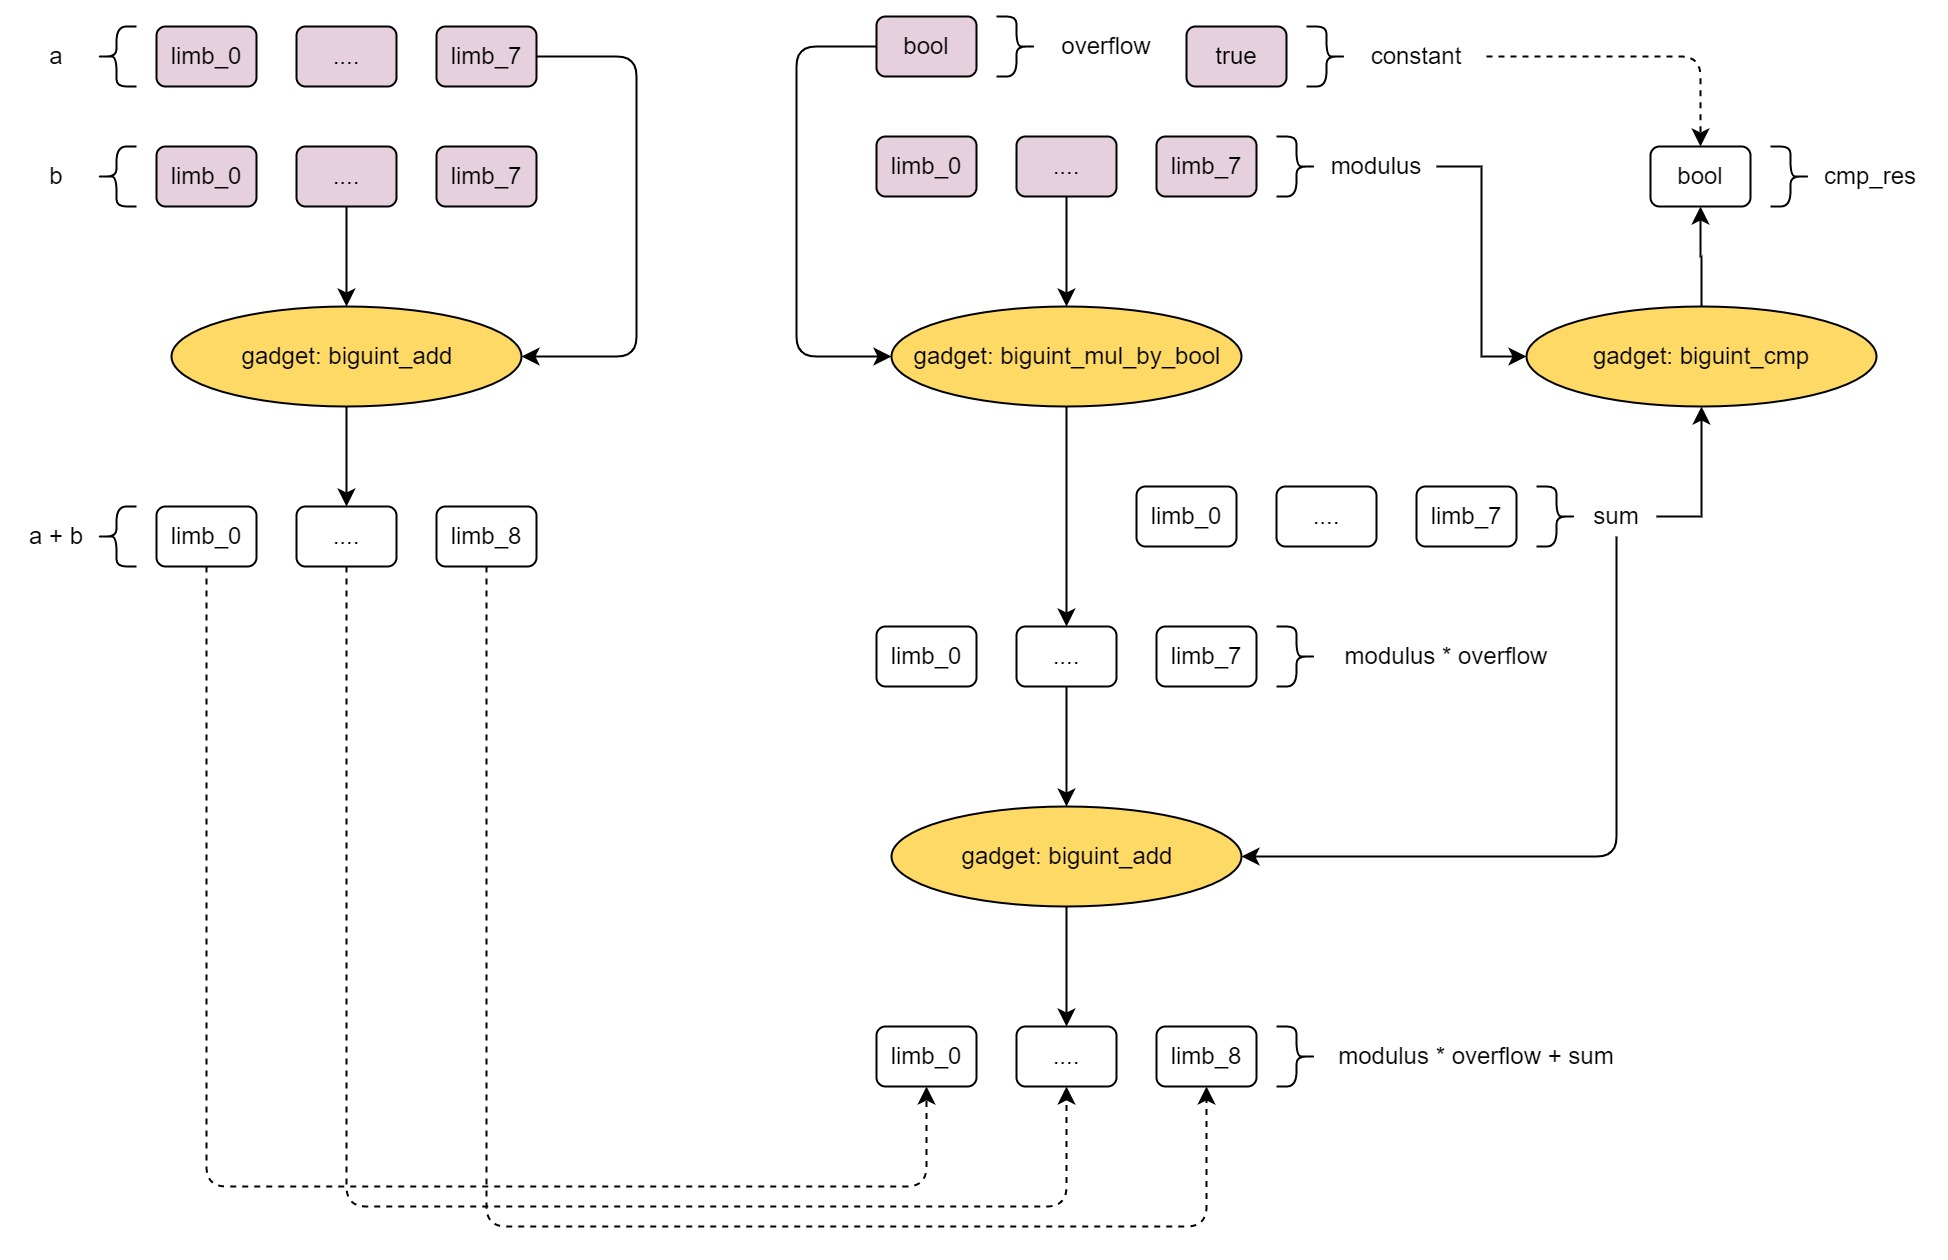
\includegraphics[width=0.6\textwidth]{nonnative-add-layout.jpg}
    \caption{non-native-add layout}
    \label{fig:non-native-add-layout}
\end{figure}

\paragraph{non-native-sub}

\begin{enumerate}
    \item \verb|Target|: Check the substrate relation among three non-native target objects.
    \item \verb|Constraints logic|:
    \begin{itemize}
        \item Check equation for gadget: \verb|diff + b = a + modular * overflow|;
        \item Check that ``overflow is bool'';
        \item Check that ``diff.limbs is range U32''.
    \end{itemize}
    \item \verb|Process layout|: See \figref{fig:non-native-sub-layout}
    \item \verb|Constraints info and costs|:
    \begin{itemize}
        \item gadget biguint-add num: 1
        \item gadget biguint-sub num: 1
        \item gadget biguint-mul-by-bool num: 1
        \item gadget u32rangecheck num: 1
        \item gadget assert-bool num: 1
        \item gate type num: 4 (U32AddManyGate, U32SubtractionGate, U32RangeCheckGate, ArithmeticGate)
        \item gate instance num: 7 = 2 (U32AddManyGate) + 2 (U32SubtractionGate) + 1 (U32RangeCheckGate) + 1 (ArithmeticGate(1,0)) + 1 (ArithmeticGate(1,-1))
        \item copy-constraints: 89 = 32{biguint-add num} + 27{U32SubtractionGate} + 9{biguint-mul-by-bool} + 8{u32rangecheck} + 4{assert-bool} + 9
    \end{itemize}
\end{enumerate}

\begin{figure}[!ht]
    \centering
    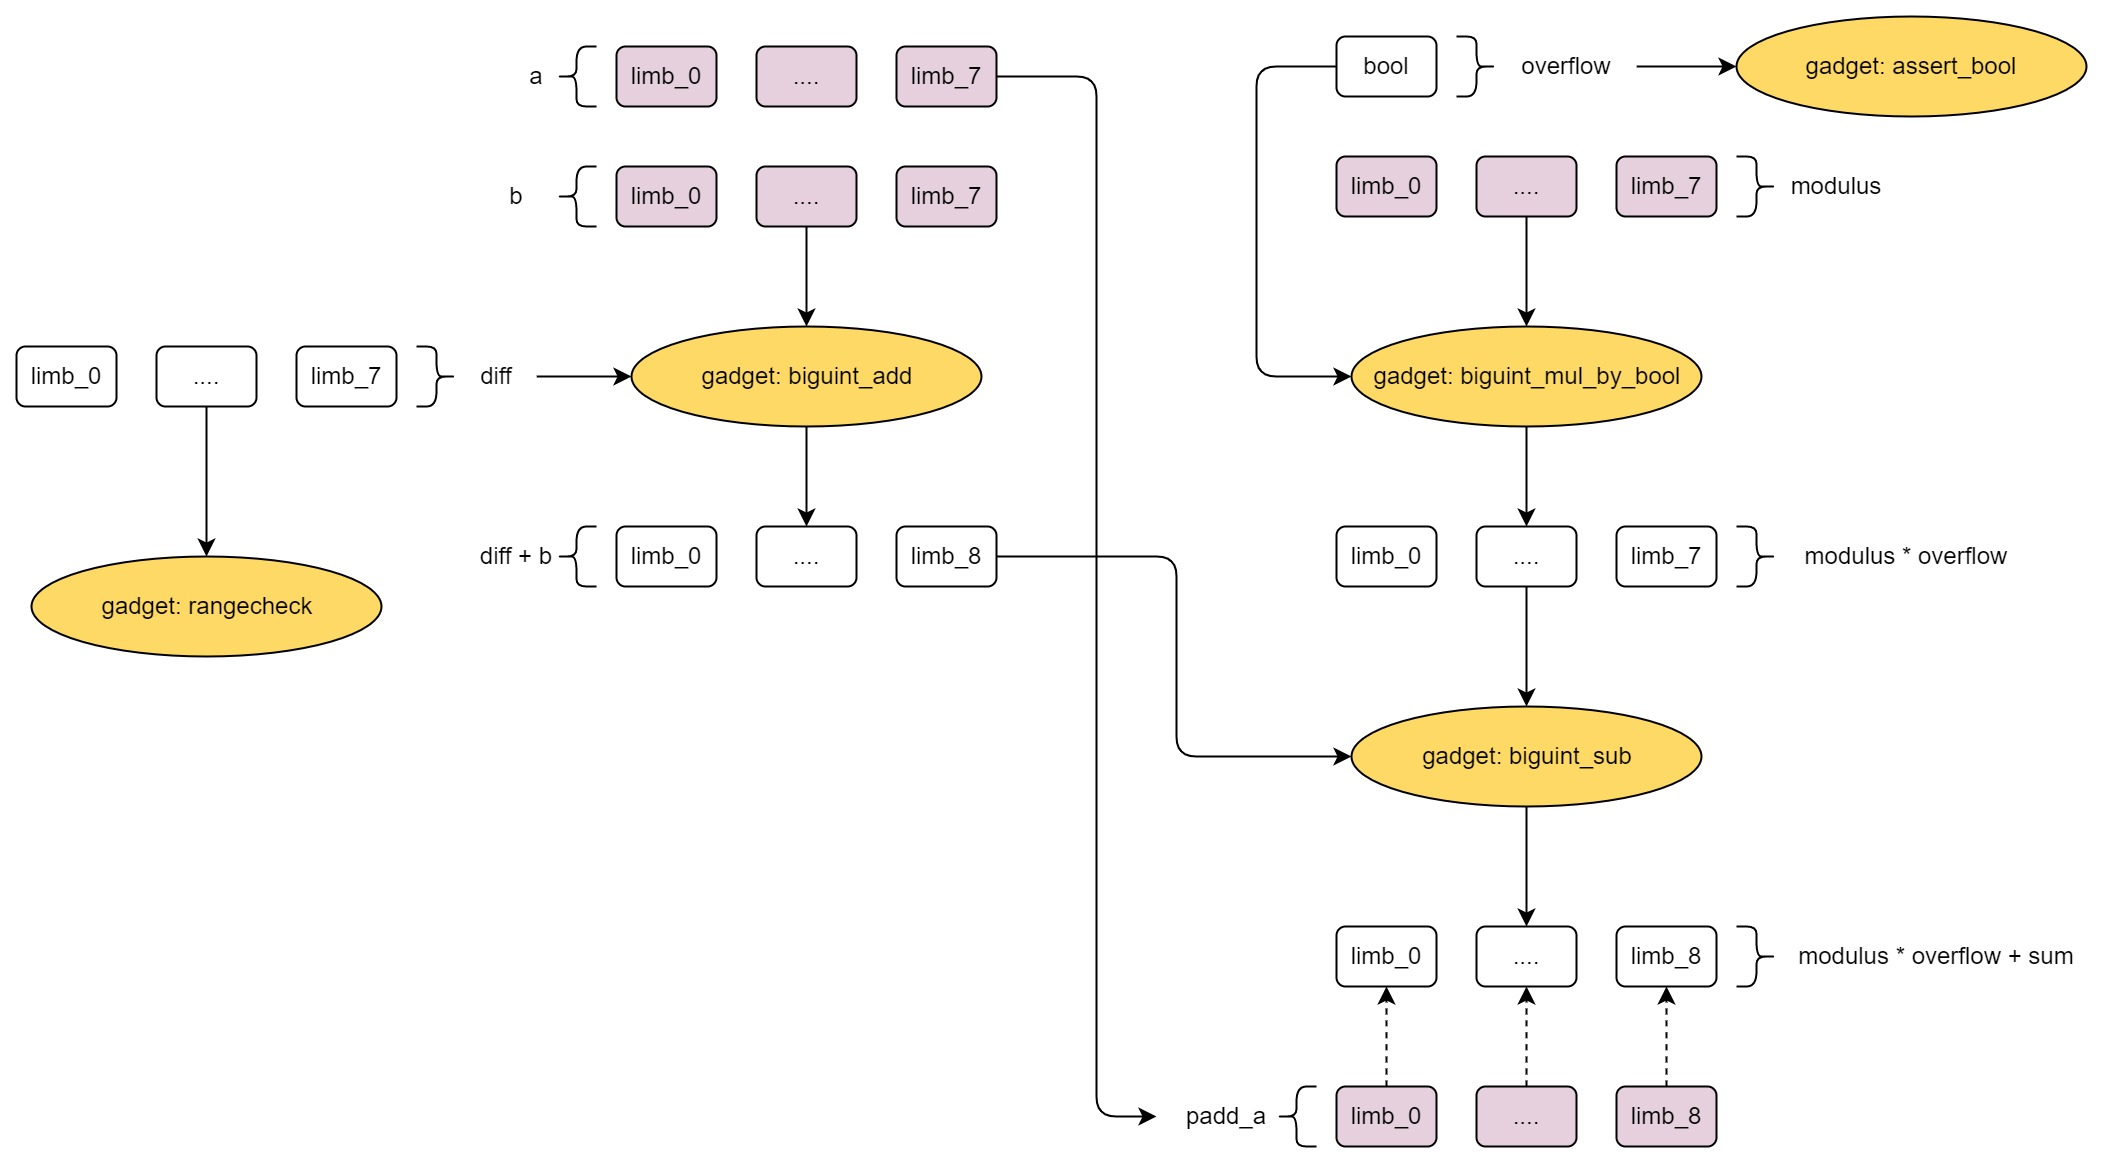
\includegraphics[width=0.6\textwidth]{nonnative-sub-layout.jpg}
    \caption{non-native-sub layout}
    \label{fig:non-native-sub-layout}
\end{figure}
\paragraph{nonnative-mul}

\subparagraph{Target}
Check the multiplication relation among three nonnative target objects.

\subparagraph{Constraints logic}
\begin{itemize}
    \item Check equation for gadget: \verb|a * b = prod + modular * overflow|;
    \item Check that ``overflow.limb is U32'';
    \item Check that ``prod.limb is U32''.
\end{itemize}

\subparagraph{Process layout}
See \figref{fig:nonnative-mul-layout}.
\begin{figure}[!ht]
    \centering
    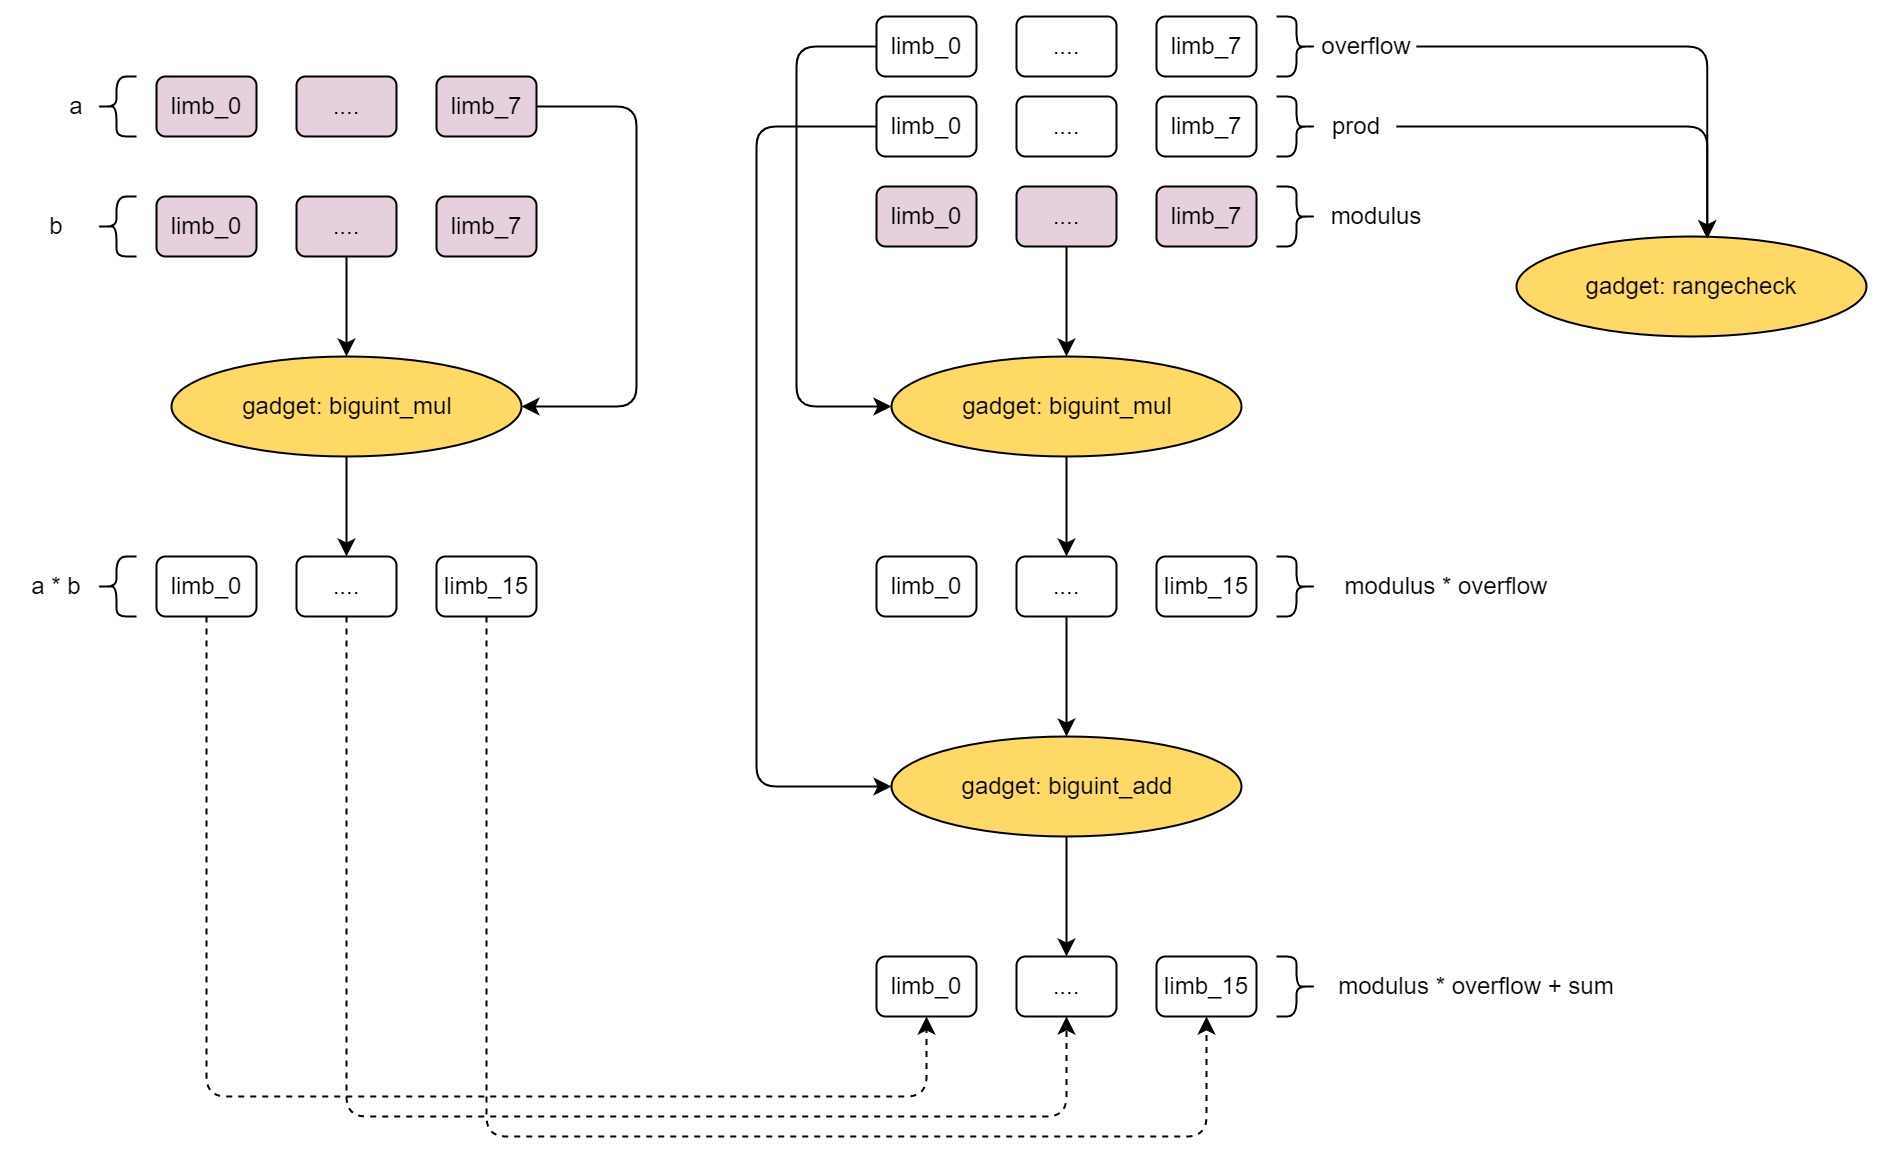
\includegraphics[width=0.6\textwidth]{nonnative-mul-layout.jpg}
    \caption{nonnative-mul layout}
    \label{fig:nonnative-mul-layout}
\end{figure}

\subparagraph{Constraints info and costs}
\begin{itemize}
    \item gadget biguint-add num: 1
    \item gadget biguint-mul num: 2
    \item gadget u32rangecheck num: 2
    \item gate type num: 9 = 7(U32AddManyGate\{3,5,7,9,11,13,15\}) + 1(U32RangeCheckGate) + 1(U32ArithmeticGate)
    \item gate instance num: 37 = 2(u32rangecheck) + 8(biguint-mul: constant-input) + 22(biguint-mul) + 1 + 3(biguint-add)
    \item copy-constraints: 583 = 8 * 2(u32rangecheck) + 3 * 3 + (4 + 6 + 8 + 10 + 12 + 14 + 16) * 4 + (8 * 8) * 3 + 17 * 4 + 18
\end{itemize}

\paragraph{nonnative-inv}

\subparagraph{Target}
Check the modular inverse relation among three nonnative target objects.

\subparagraph{Constraints logic}
\begin{itemize}
    \item Check equation for gadget: \verb|a * inv_a = 1 + modular * div|.
\end{itemize}

\subparagraph{Process layout}
See \figref{fig:nonnative-inv-layout}.
\begin{figure}[!ht]
    \centering
    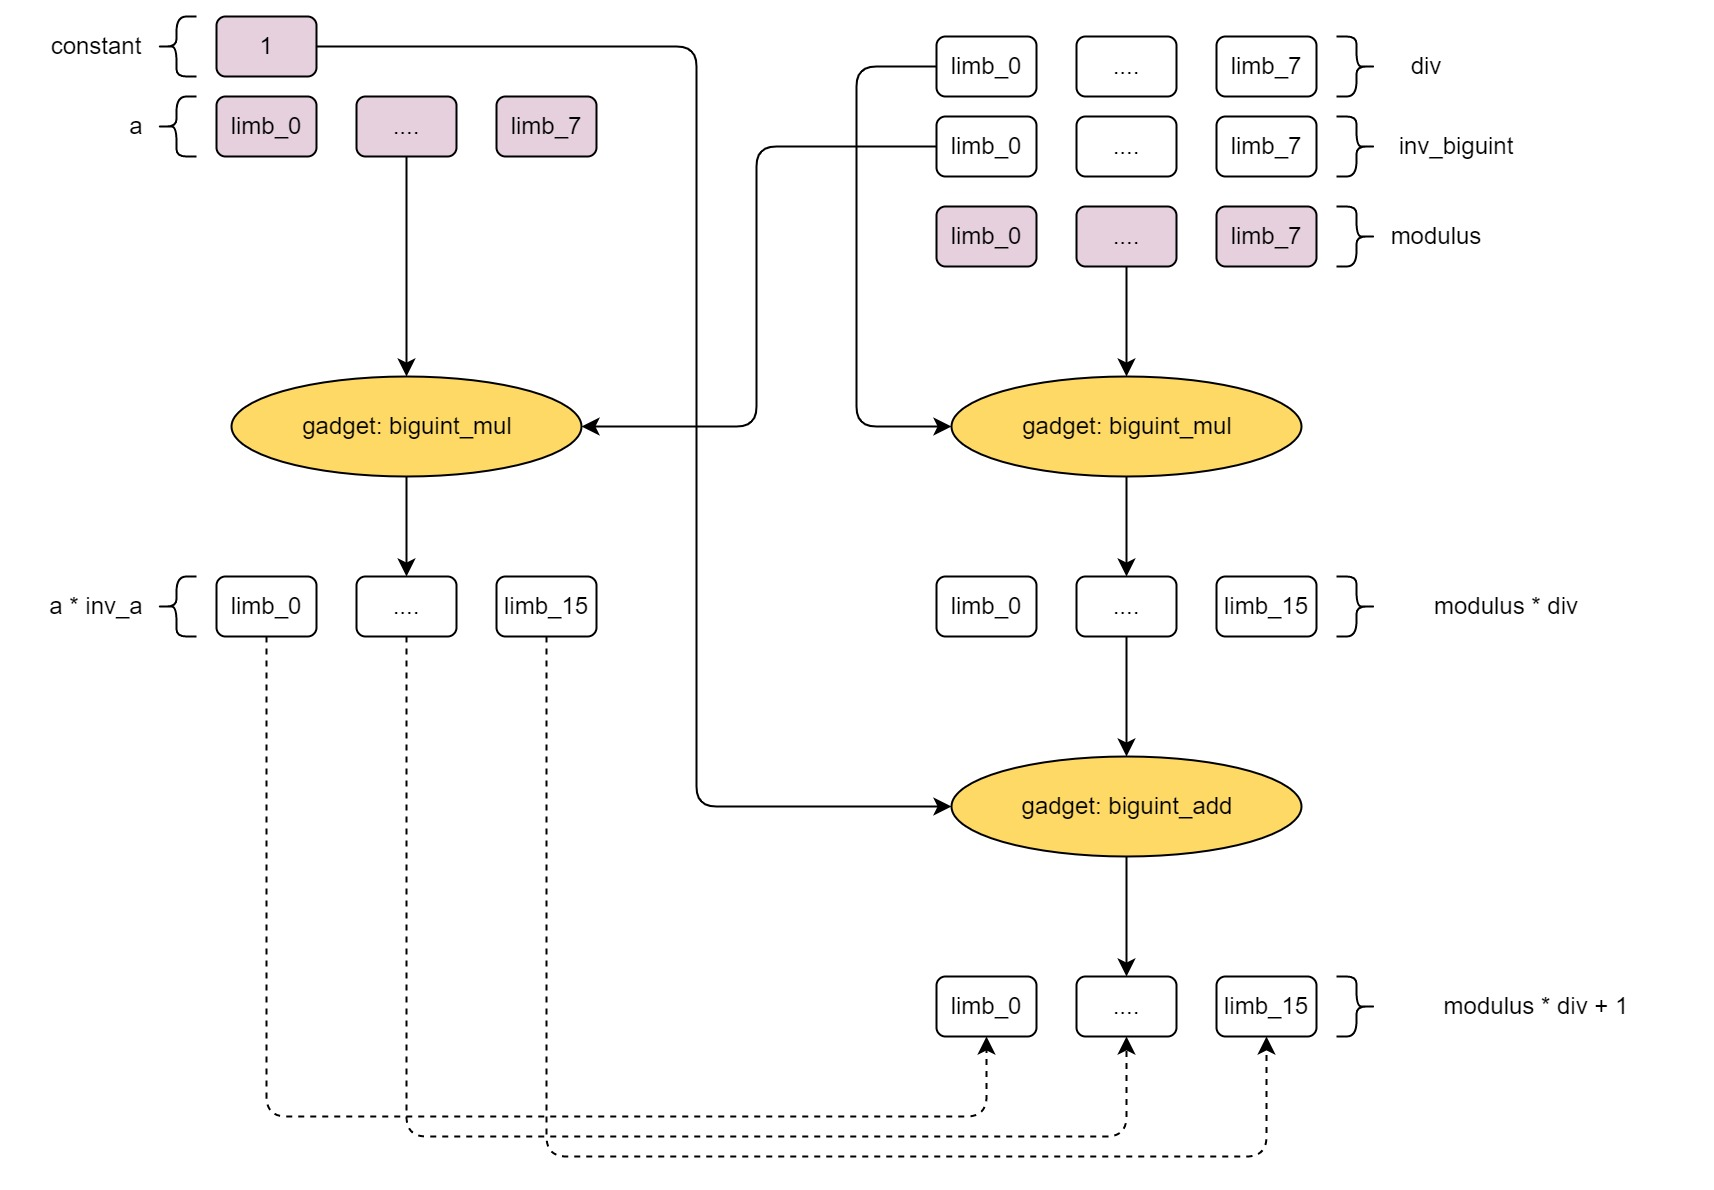
\includegraphics[width=0.8\textwidth]{nonnative-inv-layout.jpg}
    \caption{nonnative-inv layout}
    \label{fig:nonnative-inv-layout}
\end{figure}

\subparagraph{Constraints info and costs}
\begin{itemize}
    \item gadget biguint-add num: 1
    \item gadget biguint-mul num: 2
    \item gate type num: 8 = 7(U32AddManyGate\{3,5,7,9,11,13,15\}) + 1(U32ArithmeticGate)
    \item gate instance num: 56 = (8 * 8 + 2) * 2 / 3 + 5(U32AddManyGate{3}) + 5 + 2(U32AddManyGate{15})
    \item copy-constraints: 762 = (8 * 8 + 2) * 2 * 3 + 21 * 4 + (6 + 8 + 10 + 12 + 14) * 4 + 4 * 16 + 18
\end{itemize}


\paragraph{curve-add}

\subparagraph{Target}
Implement the addition of two different curve points. this is an incomplete addition, you can refer to The halo2 Book\cite{website:halo2-book} to learn more about it.

\subparagraph{Constraints logic}
$(x_1,y_1) \ne (x_2,y_2)$, See \figref{fig:curve-add}.
\begin{figure}[!ht]
    \centering
    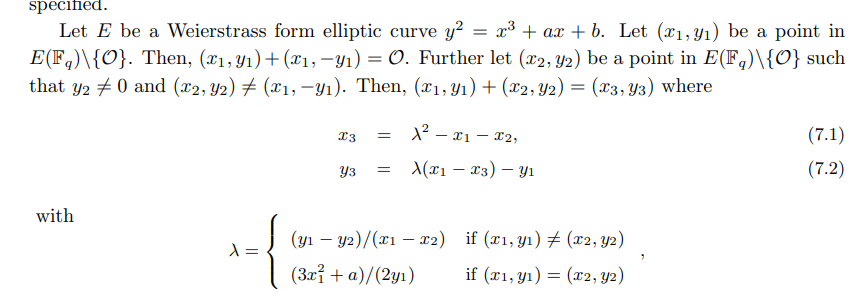
\includegraphics[width=0.6\textwidth]{curve-add.jpg}
    \caption{curve-add}
    \label{fig:curve-add}
\end{figure}

\subparagraph{Process layout}
See \figref{fig:curve-add-layout}
\begin{figure}[!ht]
    \centering
    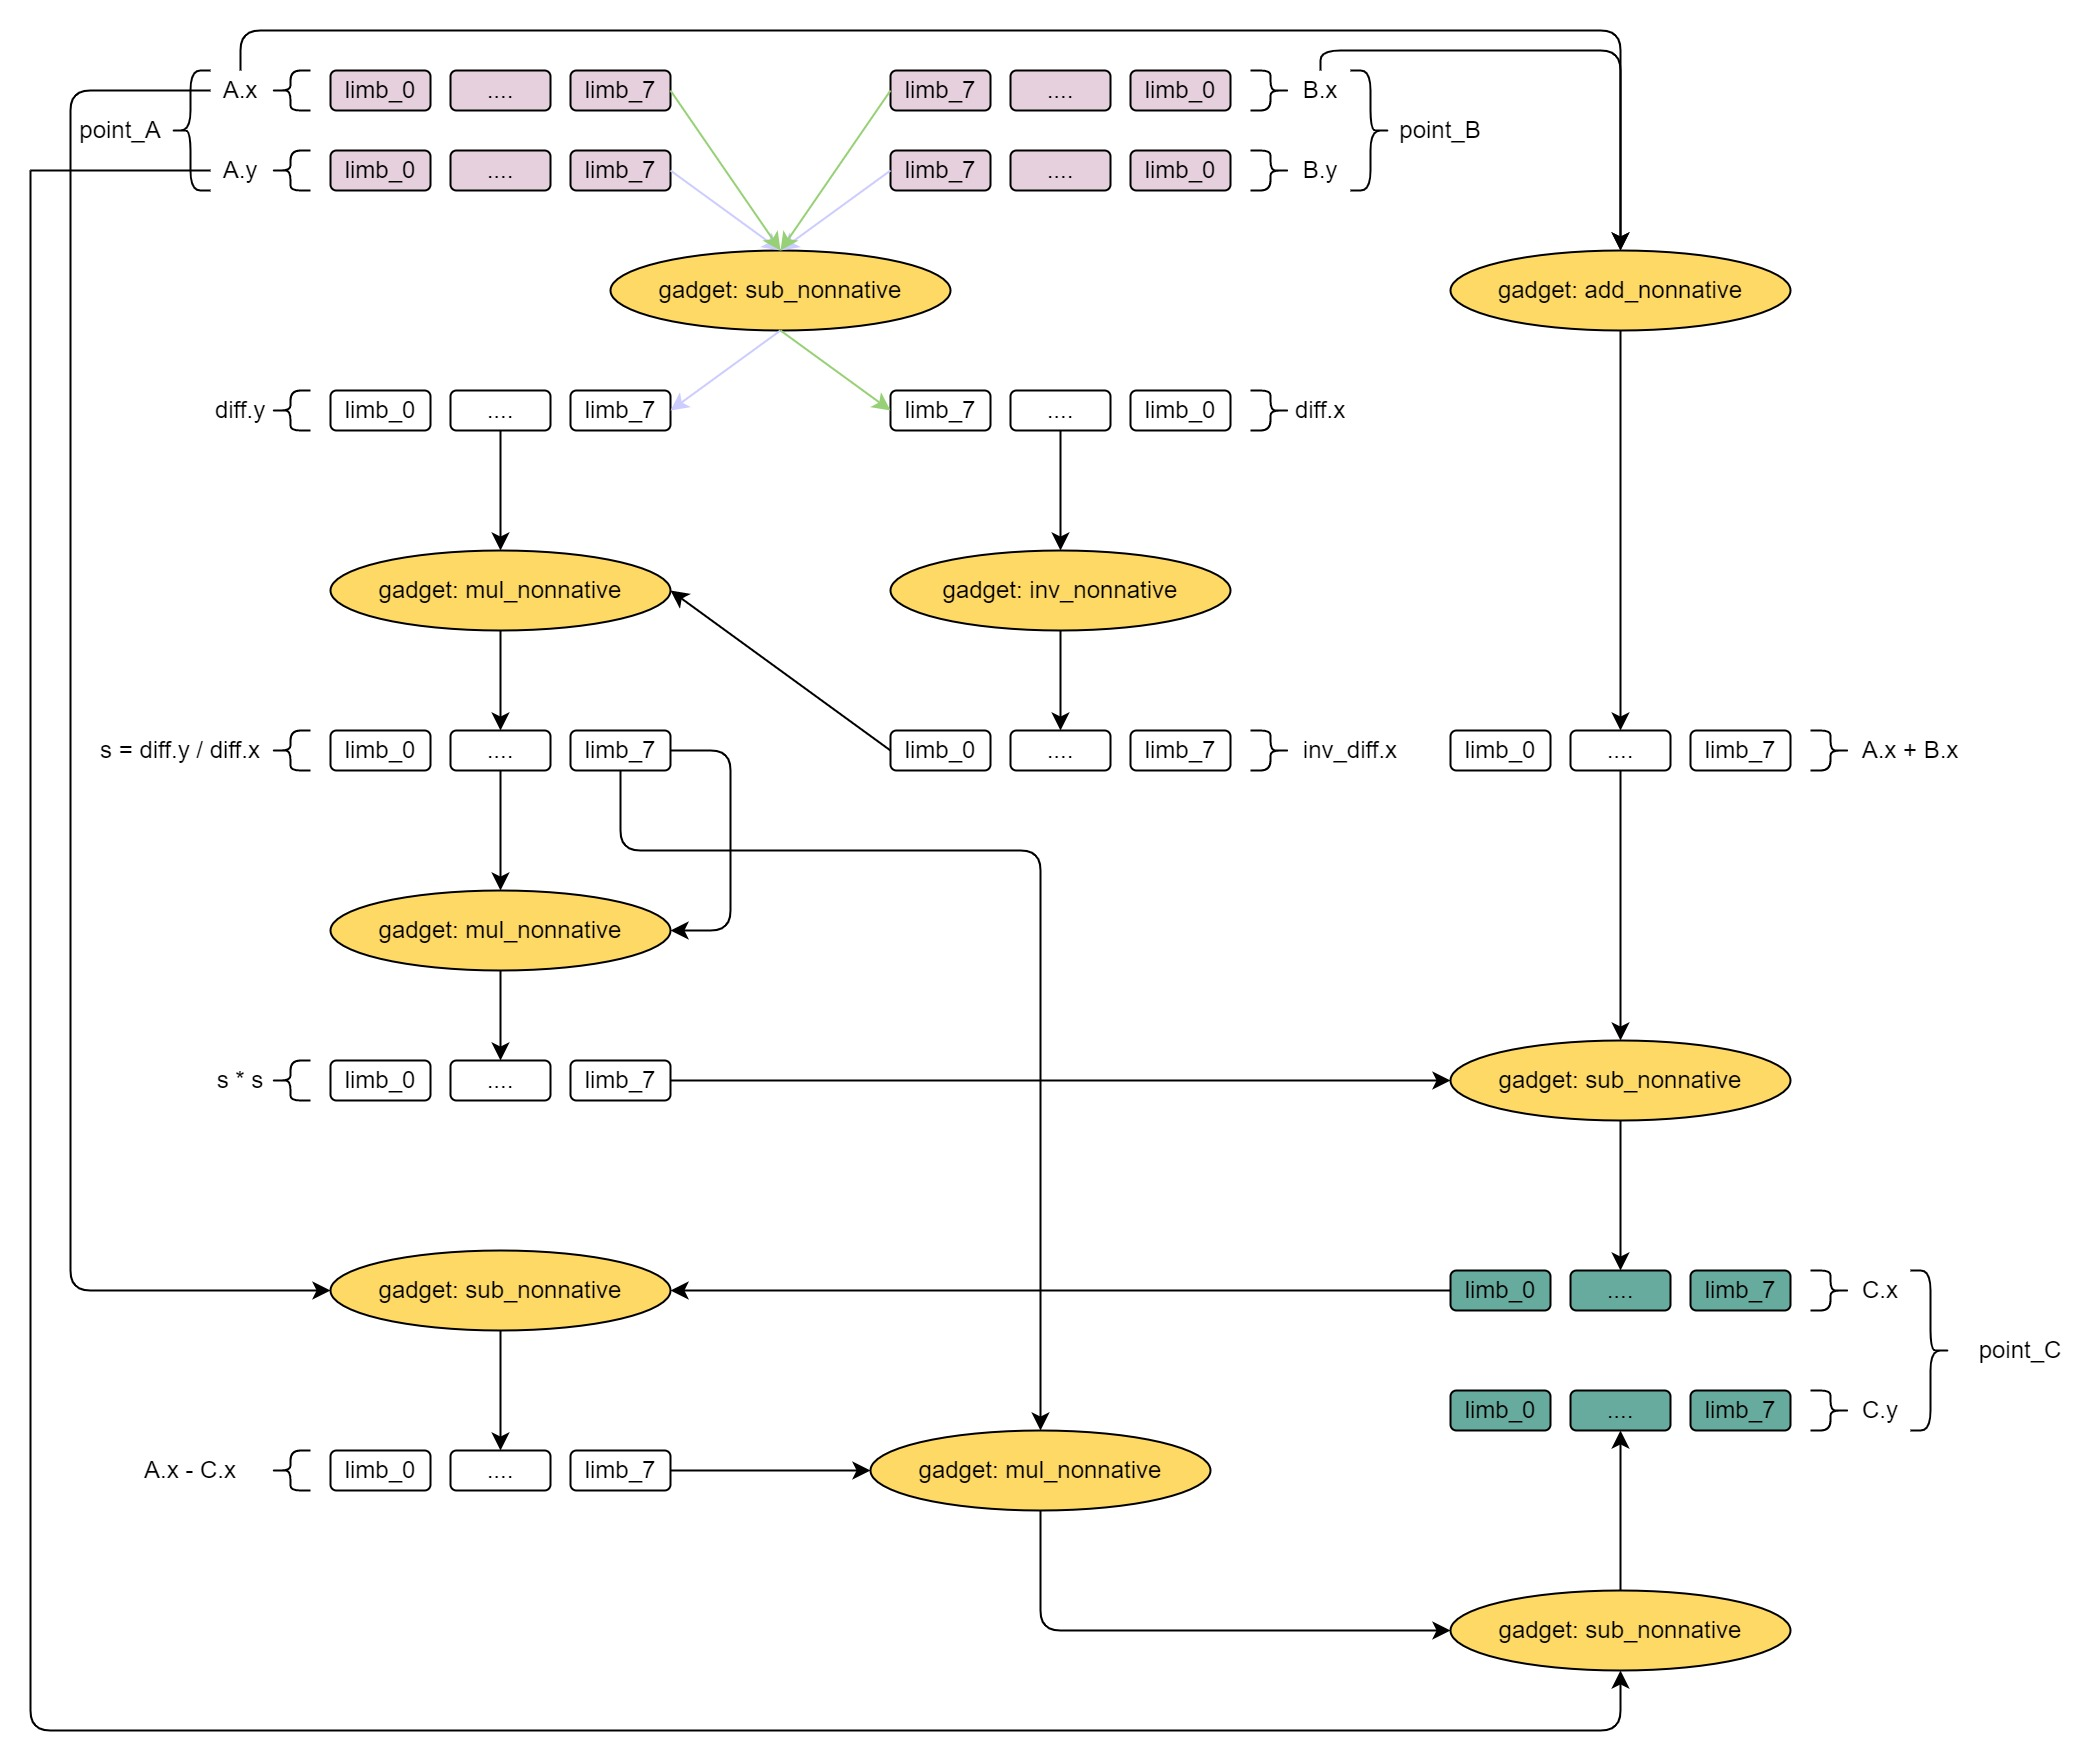
\includegraphics[width=0.6\textwidth]{curve-add-layout.jpg}
    \caption{curve-add layout}
    \label{fig:curve-add-layout}
\end{figure}

\subparagraph{Constraints info and costs}
\begin{itemize}
    \item gadget-sub-nonnative num: 5
    \item gadget-add-nonnative num: 1
    \item gadget-mul-nonnative num: 3
    \item gadget-inv-nonnative num: 1
    \item gate type num: 14
        \begin{itemize}
            \item 8: U32AddManyGate\{2,3,5,7,9,11,13,15\}
            \item 1: ComparisonGate
            \item 1: ArithmeticGate
            \item 1: U32ArithmeticGate
            \item 1: U32SubtractionGate
            \item 2: U32RangeCheckGate\{0,8\}
        \end{itemize}
\end{itemize}

\paragraph{curve-double}

\subparagraph{target}
Implement the addition of two same curve points. this is an incomplete addition, you can refer to The halo2 Book\cite{website:halo2-book} to learn more about it.

\subparagraph{Constraints logic}
$(x_1,y_1) = (x_2,y_2)$. See \figref{fig:curve-add}.

\subparagraph{Process layout}
See \figref{fig:curve-double-layout}.
\begin{figure}[!ht]
    \centering
    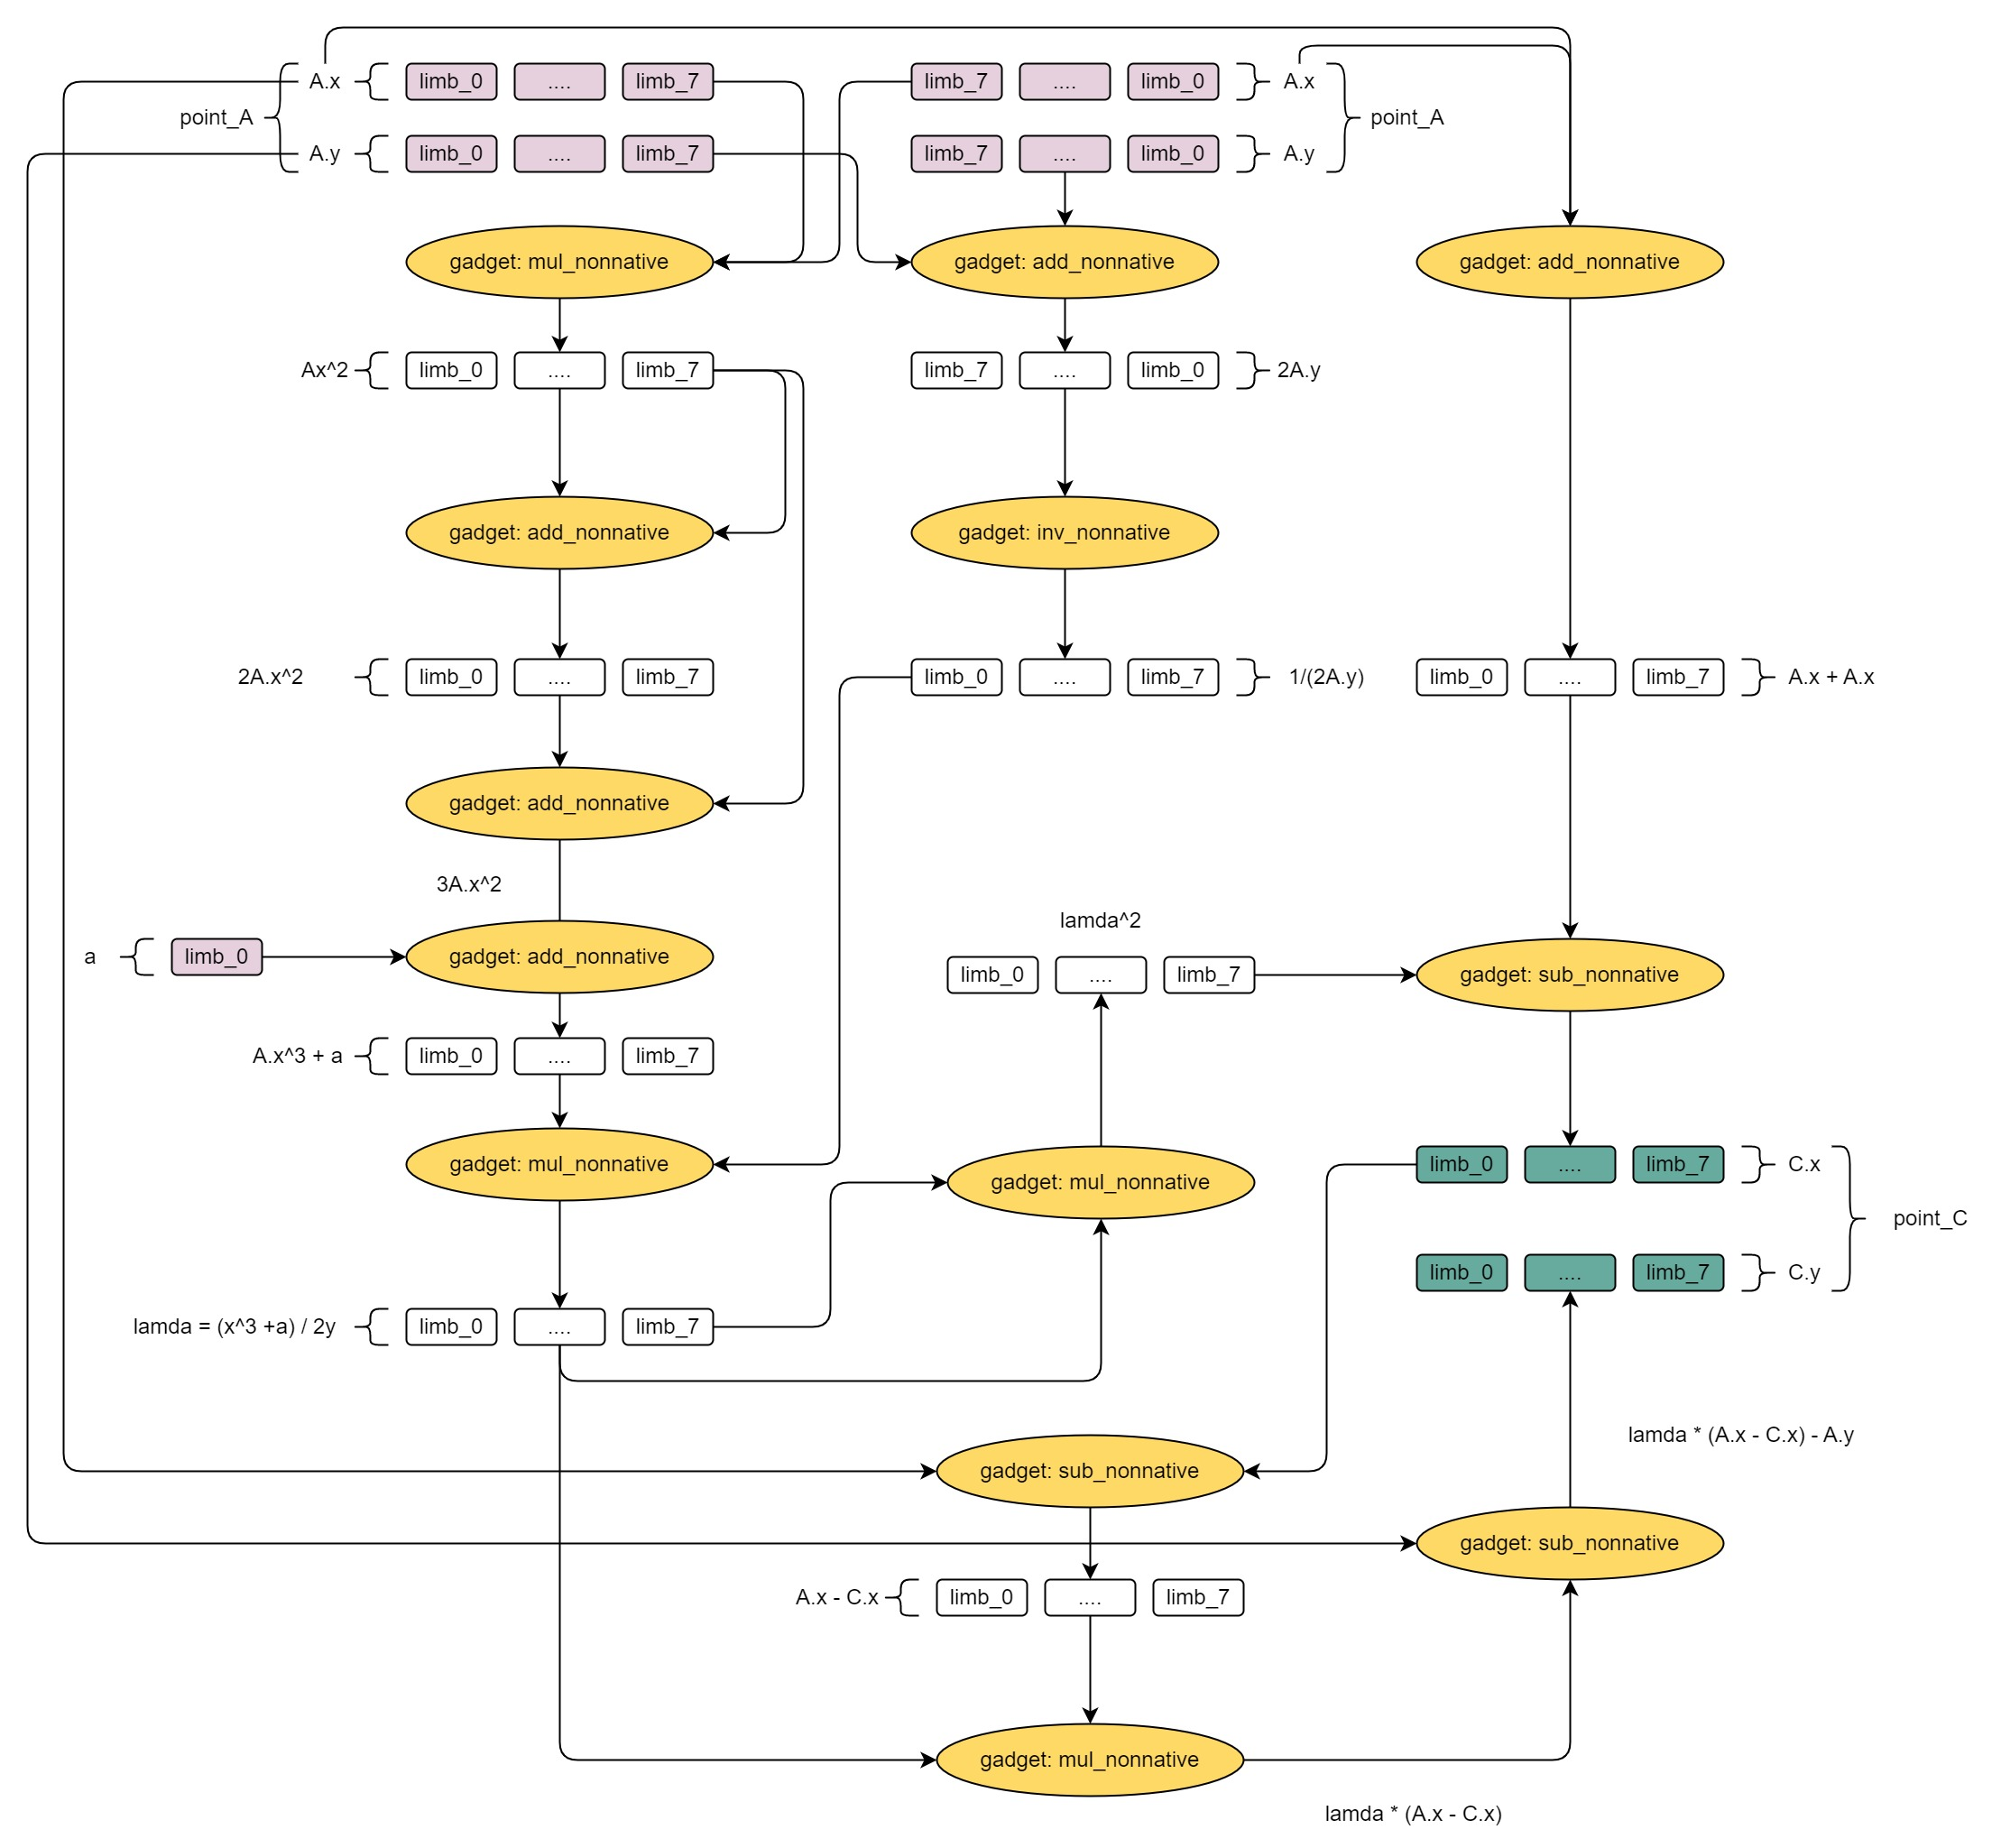
\includegraphics[width=0.6\textwidth]{curve-double-layout.jpg}
    \caption{curve-double layout}
    \label{fig:curve-double-layout}
\end{figure}

\subparagraph{Constraints info and costs}
\begin{itemize}
    \item gadget-sub-nonnative num: 3
    \item gadget-add-nonnative num: 5
    \item gadget-mul-nonnative num: 4
    \item gadget-inv-nonnative num: 1
    \item gate type num: 14
        \begin{itemize}
            \item 8: U32AddManyGate\{2,3,5,7,9,11,13,15\}
            \item 1: ComparisonGate
            \item 1: ArithmeticGate
            \item 1: U32ArithmeticGate
            \item 1: U32SubtractionGate
            \item 2: U32RangeCheckGate\{0,8\}
        \end{itemize}
\end{itemize}

\paragraph{curve-assert-valid}

\subparagraph{Target}
Check point is on the curve $y^2 = x^3 + ax + b$.

\subparagraph{Process layout}
See \figref{fig:curve-assert-valid-layout}.
\begin{figure}[!ht]
    \centering
    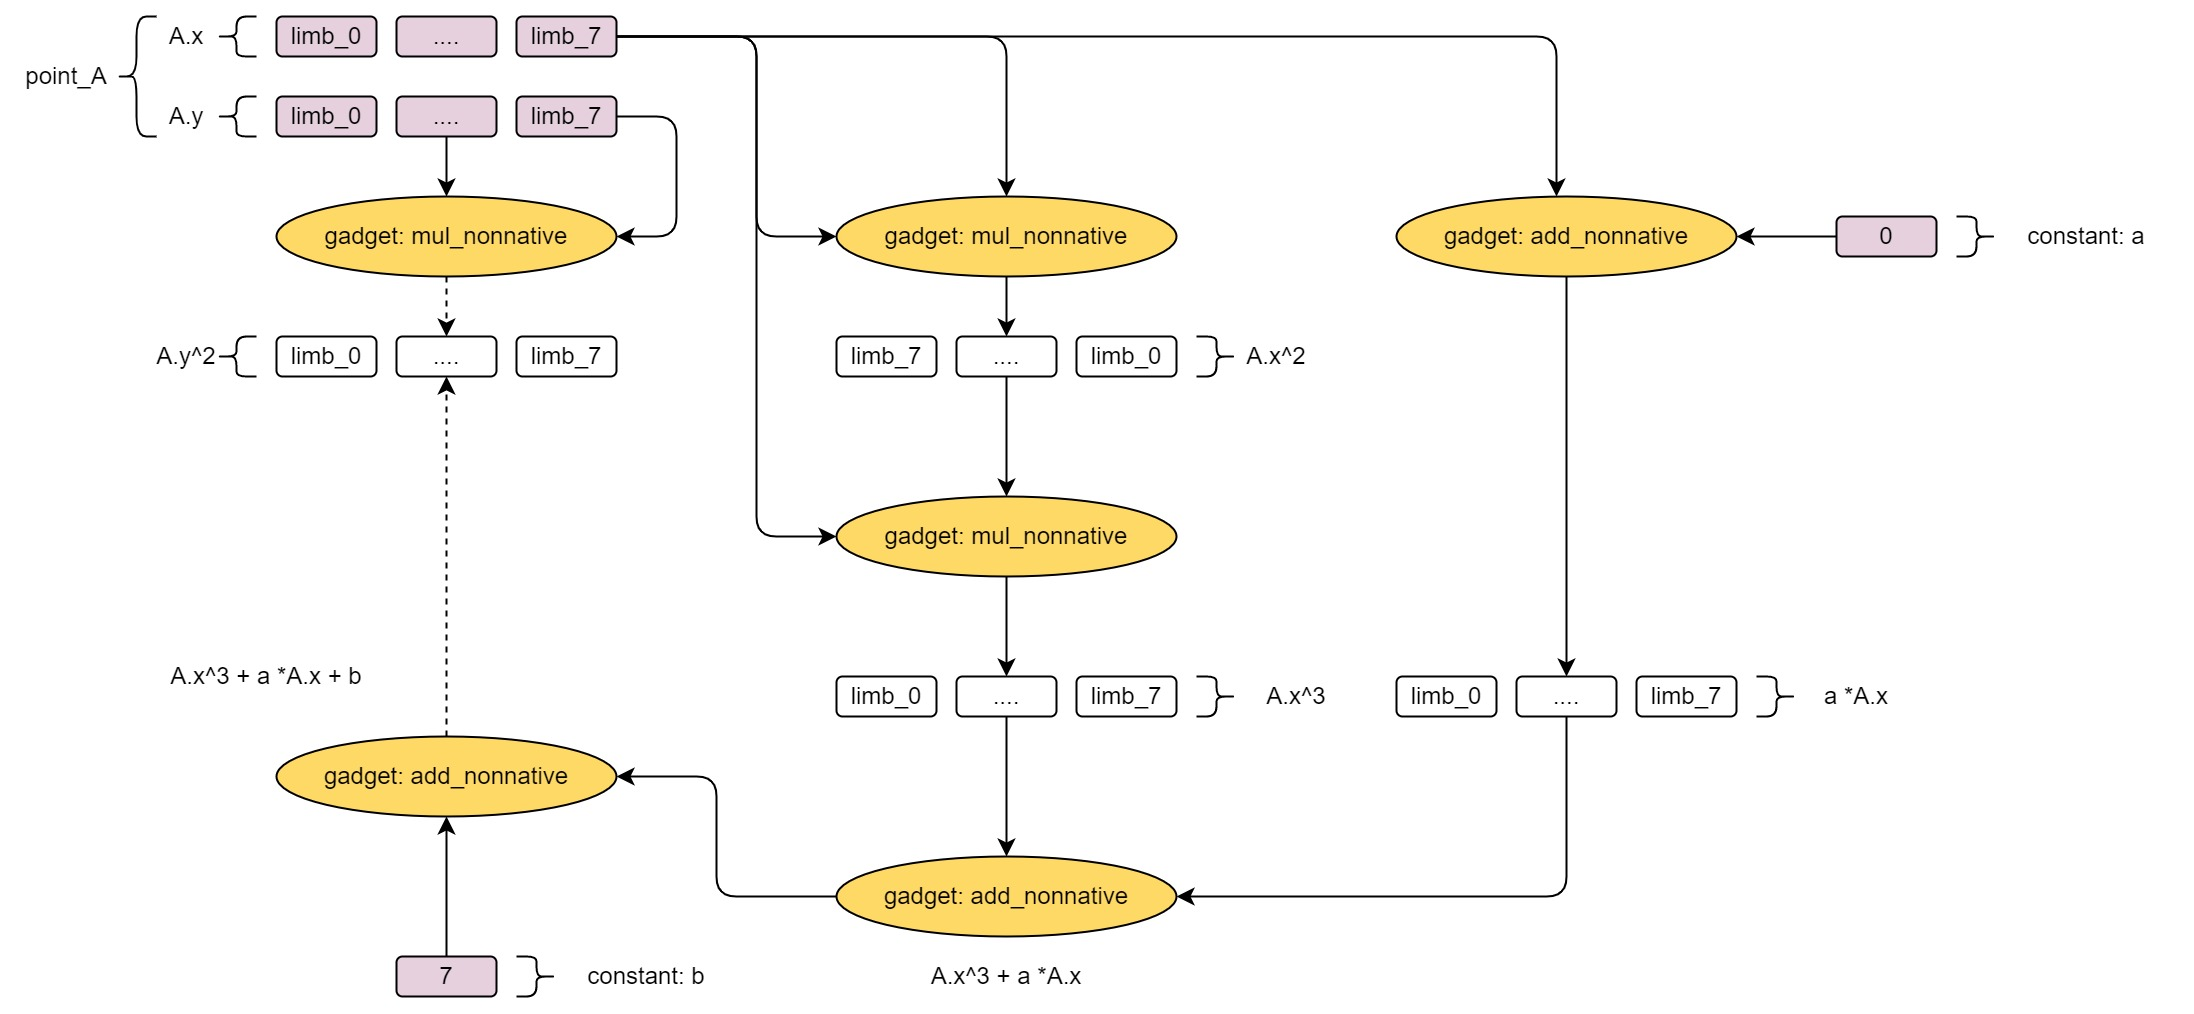
\includegraphics[width=0.5\textwidth]{curve-assert-valid-layout.jpg}
    \caption{curve-assert valid layout}
    \label{fig:curve-assert-valid-layout}
\end{figure}

\subparagraph{Constraints info and costs}
\begin{itemize}
    \item gadget-add-nonnative num: 3
    \item gadget-mul-nonnative num: 3
    \item gate type num: 13
        \begin{itemize}
            \item 8: U32AddManyGate\{2,3,5,7,9,11,13,15\}
            \item 1: ComparisonGate
            \item 1: ArithmeticGate
            \item 1: U32ArithmeticGate
            \item 2: U32RangeCheckGate\{0,8\}
        \end{itemize}
\end{itemize}
  
\paragraph{curve-msm}

\subparagraph{target}
Implement the multiplication scalar multiplication (MSM).

\subparagraph{Constraints logic}
See \figref{fig:curve-msm}.
\begin{figure}[!ht]
    \centering
    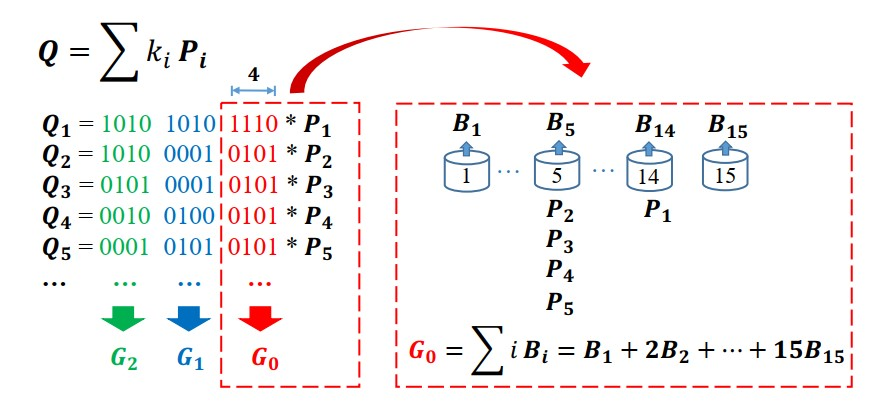
\includegraphics[width=0.5\textwidth]{curve-msm.jpg}
    \caption{curve-msm}
    \label{fig:curve-msm}
\end{figure}

\subparagraph{Constraints info and costs}
\begin{itemize}
    \item gate type num: 14
    \item gate instance num: 147553
\end{itemize}

\subsubsubsection{curve-scalar}

\begin{enumerate}
    \item \verb|Target|: Implement the multiplication between scalar and point.
    \item \verb|Constraints logic|: See \figref{fig:curve-scalar}.
    \item \verb|Constraints info and costs|:
    \begin{itemize}
        \item gate type num: 13 
        \item gate instance num: 180364          
    \end{itemize}
\end{enumerate}

\begin{figure}[!ht]
    \centering
    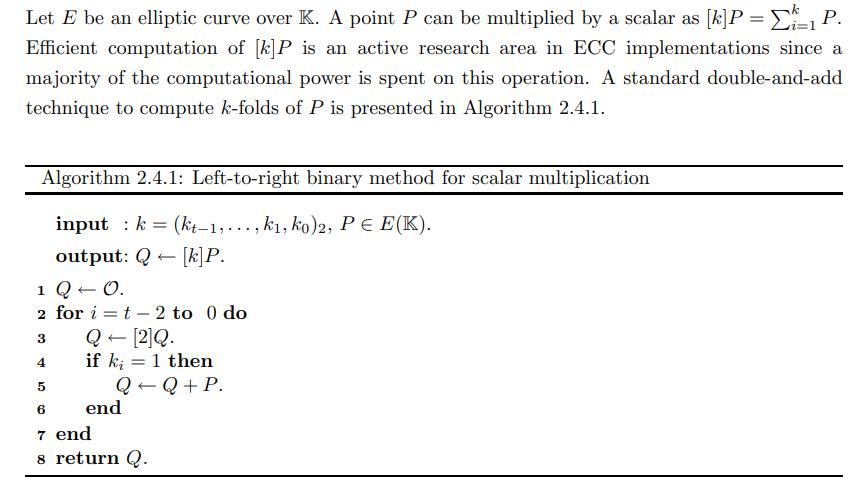
\includegraphics[width=0.6\textwidth]{curve-scalar.jpg}
    \caption{curve-scalar}
    \label{fig:curve-scalar}
\end{figure}


\paragraph{ecdsa}

\subparagraph{Target}
Implement ecdsa verify process.

\subparagraph{Constraints logic}
\begin{figure}[!ht]
    \centering
    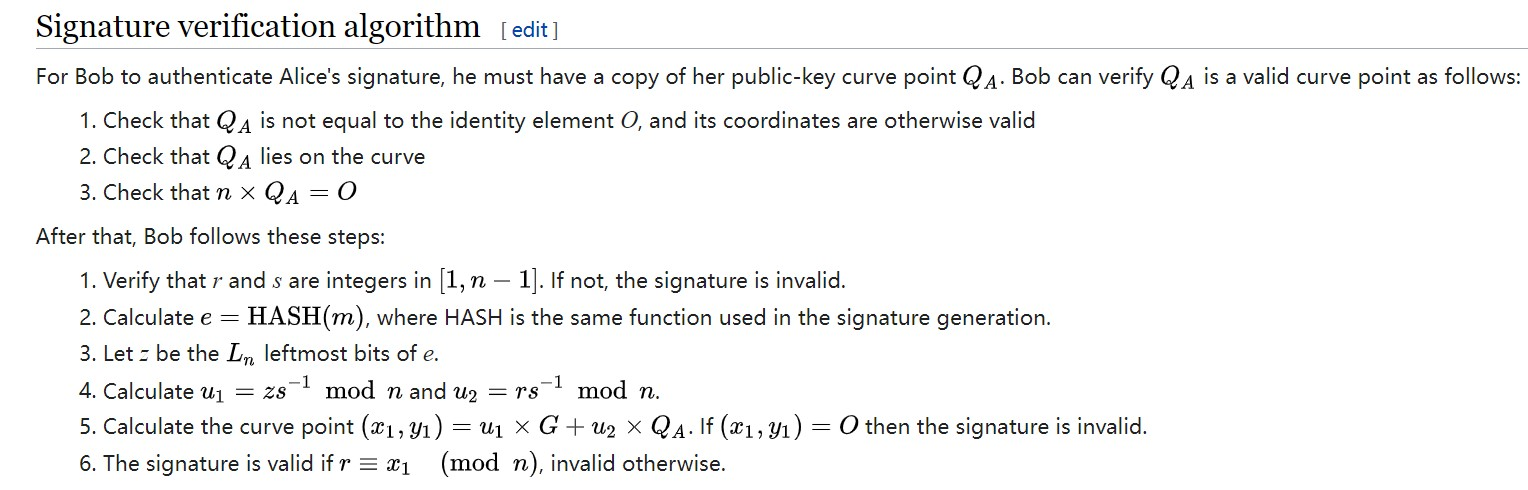
\includegraphics[width=0.5\textwidth]{ecdsa.jpg}
    \caption{ecdsa}
    \label{fig:ecdsa}
\end{figure}

\subparagraph{Constraints info and costs}
\begin{itemize}
    \item gate type num: 16
    \item gate instance num: 98039
\end{itemize}




